% Options for packages loaded elsewhere
\PassOptionsToPackage{unicode}{hyperref}
\PassOptionsToPackage{hyphens}{url}
\PassOptionsToPackage{dvipsnames,svgnames,x11names}{xcolor}
%
\documentclass[
  letterpaper,
  DIV=11,
  numbers=noendperiod]{scrartcl}

\usepackage{amsmath,amssymb}
\usepackage{iftex}
\ifPDFTeX
  \usepackage[T1]{fontenc}
  \usepackage[utf8]{inputenc}
  \usepackage{textcomp} % provide euro and other symbols
\else % if luatex or xetex
  \usepackage{unicode-math}
  \defaultfontfeatures{Scale=MatchLowercase}
  \defaultfontfeatures[\rmfamily]{Ligatures=TeX,Scale=1}
\fi
\usepackage{lmodern}
\ifPDFTeX\else  
    % xetex/luatex font selection
\fi
% Use upquote if available, for straight quotes in verbatim environments
\IfFileExists{upquote.sty}{\usepackage{upquote}}{}
\IfFileExists{microtype.sty}{% use microtype if available
  \usepackage[]{microtype}
  \UseMicrotypeSet[protrusion]{basicmath} % disable protrusion for tt fonts
}{}
\makeatletter
\@ifundefined{KOMAClassName}{% if non-KOMA class
  \IfFileExists{parskip.sty}{%
    \usepackage{parskip}
  }{% else
    \setlength{\parindent}{0pt}
    \setlength{\parskip}{6pt plus 2pt minus 1pt}}
}{% if KOMA class
  \KOMAoptions{parskip=half}}
\makeatother
\usepackage{xcolor}
\setlength{\emergencystretch}{3em} % prevent overfull lines
\setcounter{secnumdepth}{3}
% Make \paragraph and \subparagraph free-standing
\makeatletter
\ifx\paragraph\undefined\else
  \let\oldparagraph\paragraph
  \renewcommand{\paragraph}{
    \@ifstar
      \xxxParagraphStar
      \xxxParagraphNoStar
  }
  \newcommand{\xxxParagraphStar}[1]{\oldparagraph*{#1}\mbox{}}
  \newcommand{\xxxParagraphNoStar}[1]{\oldparagraph{#1}\mbox{}}
\fi
\ifx\subparagraph\undefined\else
  \let\oldsubparagraph\subparagraph
  \renewcommand{\subparagraph}{
    \@ifstar
      \xxxSubParagraphStar
      \xxxSubParagraphNoStar
  }
  \newcommand{\xxxSubParagraphStar}[1]{\oldsubparagraph*{#1}\mbox{}}
  \newcommand{\xxxSubParagraphNoStar}[1]{\oldsubparagraph{#1}\mbox{}}
\fi
\makeatother


\providecommand{\tightlist}{%
  \setlength{\itemsep}{0pt}\setlength{\parskip}{0pt}}\usepackage{longtable,booktabs,array}
\usepackage{calc} % for calculating minipage widths
% Correct order of tables after \paragraph or \subparagraph
\usepackage{etoolbox}
\makeatletter
\patchcmd\longtable{\par}{\if@noskipsec\mbox{}\fi\par}{}{}
\makeatother
% Allow footnotes in longtable head/foot
\IfFileExists{footnotehyper.sty}{\usepackage{footnotehyper}}{\usepackage{footnote}}
\makesavenoteenv{longtable}
\usepackage{graphicx}
\makeatletter
\def\maxwidth{\ifdim\Gin@nat@width>\linewidth\linewidth\else\Gin@nat@width\fi}
\def\maxheight{\ifdim\Gin@nat@height>\textheight\textheight\else\Gin@nat@height\fi}
\makeatother
% Scale images if necessary, so that they will not overflow the page
% margins by default, and it is still possible to overwrite the defaults
% using explicit options in \includegraphics[width, height, ...]{}
\setkeys{Gin}{width=\maxwidth,height=\maxheight,keepaspectratio}
% Set default figure placement to htbp
\makeatletter
\def\fps@figure{htbp}
\makeatother
% definitions for citeproc citations
\NewDocumentCommand\citeproctext{}{}
\NewDocumentCommand\citeproc{mm}{%
  \begingroup\def\citeproctext{#2}\cite{#1}\endgroup}
\makeatletter
 % allow citations to break across lines
 \let\@cite@ofmt\@firstofone
 % avoid brackets around text for \cite:
 \def\@biblabel#1{}
 \def\@cite#1#2{{#1\if@tempswa , #2\fi}}
\makeatother
\newlength{\cslhangindent}
\setlength{\cslhangindent}{1.5em}
\newlength{\csllabelwidth}
\setlength{\csllabelwidth}{3em}
\newenvironment{CSLReferences}[2] % #1 hanging-indent, #2 entry-spacing
 {\begin{list}{}{%
  \setlength{\itemindent}{0pt}
  \setlength{\leftmargin}{0pt}
  \setlength{\parsep}{0pt}
  % turn on hanging indent if param 1 is 1
  \ifodd #1
   \setlength{\leftmargin}{\cslhangindent}
   \setlength{\itemindent}{-1\cslhangindent}
  \fi
  % set entry spacing
  \setlength{\itemsep}{#2\baselineskip}}}
 {\end{list}}
\usepackage{calc}
\newcommand{\CSLBlock}[1]{\hfill\break\parbox[t]{\linewidth}{\strut\ignorespaces#1\strut}}
\newcommand{\CSLLeftMargin}[1]{\parbox[t]{\csllabelwidth}{\strut#1\strut}}
\newcommand{\CSLRightInline}[1]{\parbox[t]{\linewidth - \csllabelwidth}{\strut#1\strut}}
\newcommand{\CSLIndent}[1]{\hspace{\cslhangindent}#1}

\usepackage{booktabs}
\usepackage{caption}
\usepackage{longtable}
\usepackage{colortbl}
\usepackage{array}
\usepackage{anyfontsize}
\usepackage{multirow}
\usepackage{amsmath, booktabs, caption, longtable, xcolor, ulem}
\KOMAoption{captions}{tableheading}
\makeatletter
\@ifpackageloaded{caption}{}{\usepackage{caption}}
\AtBeginDocument{%
\ifdefined\contentsname
  \renewcommand*\contentsname{Table of contents}
\else
  \newcommand\contentsname{Table of contents}
\fi
\ifdefined\listfigurename
  \renewcommand*\listfigurename{List of Figures}
\else
  \newcommand\listfigurename{List of Figures}
\fi
\ifdefined\listtablename
  \renewcommand*\listtablename{List of Tables}
\else
  \newcommand\listtablename{List of Tables}
\fi
\ifdefined\figurename
  \renewcommand*\figurename{Figure}
\else
  \newcommand\figurename{Figure}
\fi
\ifdefined\tablename
  \renewcommand*\tablename{Table}
\else
  \newcommand\tablename{Table}
\fi
}
\@ifpackageloaded{float}{}{\usepackage{float}}
\floatstyle{ruled}
\@ifundefined{c@chapter}{\newfloat{codelisting}{h}{lop}}{\newfloat{codelisting}{h}{lop}[chapter]}
\floatname{codelisting}{Listing}
\newcommand*\listoflistings{\listof{codelisting}{List of Listings}}
\makeatother
\makeatletter
\makeatother
\makeatletter
\@ifpackageloaded{caption}{}{\usepackage{caption}}
\@ifpackageloaded{subcaption}{}{\usepackage{subcaption}}
\makeatother

\ifLuaTeX
  \usepackage{selnolig}  % disable illegal ligatures
\fi
\usepackage{bookmark}

\IfFileExists{xurl.sty}{\usepackage{xurl}}{} % add URL line breaks if available
\urlstyle{same} % disable monospaced font for URLs
\hypersetup{
  pdftitle={msqrob2TMT: robust linear mixed models for inferring differential abundant proteins in labelled experiments with arbitrarily complex design},
  pdfauthor={, , , , and },
  colorlinks=true,
  linkcolor={blue},
  filecolor={Maroon},
  citecolor={Blue},
  urlcolor={Blue},
  pdfcreator={LaTeX via pandoc}}


\title{msqrob2TMT: robust linear mixed models for inferring differential
abundant proteins in labelled experiments with arbitrarily complex
design}
\author{Stijn
Vandenbulcke\textsuperscript{$\dagger{}$,1,2,3} \and Christophe
Vanderaa\textsuperscript{$\dagger{}$,1} \and Oliver
Crook\textsuperscript{4} \and Lennart
Martens\textsuperscript{2,3} \and Lieven Clement\textsuperscript{1,*}}
\date{}

\begin{document}
\maketitle


\textsuperscript{$\dagger{}$}
These authors contributed equally to this work.

\textsuperscript{1} Department of Mathematics, Computer Science and
Statistics, Ghent University, Ghent, Belgium\\
\textsuperscript{2} CompOmics, VIB Center for Medical Biotechnology,
VIB, Ghent, Belgium\\
\textsuperscript{3} Department of Biomolecular Medicine, Faculty of
Medicine and Health Sciences, Ghent University, Ghent, Belgium\\
\textsuperscript{4} Department of Statistics, University of Oxford,
Oxford, UK.

\textsuperscript{*} Correspondence:
\href{mailto:lieven.clement@ugent.be}{Lieven Clement
\textless{}lieven.clement@ugent.be\textgreater{}}

\captionsetup{labelfont=bf}
\setcapindent{0pt}

\section*{Abstract}

Labelling strategies in mass spectrometry (MS)-based proteomics enhance
sample throughput by enabling the acquisition of multiplexed samples
within a single run. However, contemporary experiments often involve
increasingly complex designs, where the number of samples exceeds the
capacity of a single run, resulting in a complex correlation structure
that must be addressed for accurate statistical inference and reliable
biomarker discovery. To this end, we introduce msqrob2TMT, a suite of
mixed model-based workflows specifically designed for differential
abundance analysis in labelled MS-based proteomics data. msqrob2TMT
accommodates both sample-specific and feature-specific (e.g., peptide or
protein) covariates, facilitating inference in experiments with
arbitrarily complex designs and allowing for explicit correction of
feature-specific covariates. We benchmark our innovative workflows
against state-of-the-art tools, including DEqMS, MSstatsTMT, and
msTrawler, using two spike-in studies. Our findings demonstrate that
msqrob2TMT offers greater flexibility, improved modularity, and enhanced
performance, particularly through the application of robust ridge
regression. Finally, we demonstrate the practical relevance of
msqrob2TMT in a real mouse study, highlighting its capacity to
effectively account for the complex correlation structure in the data.

\section{Introduction}

High-throughput LC-MS-based proteomic workflows are widely used to
quantify differential protein abundance across samples. Relative protein
quantification is generally achieved through either label-free or
labelled workflows. The latter employ stable isotope labelling
techniques such as metabolic and post-metabolic labelling, which gained
traction in recent years (Li et al. 2021). Compared to label-free
approaches, labelling offers the advantage of mitigating run-to-run
variability in peptide identification and quantification by pooling and
analysing multiple samples within a single run. This enables researchers
to compare proteomes across multiple conditions or treatments within a
single MS run, thereby providing a more comprehensive view of the
proteome and enhancing the statistical power of the analysis. Current
tandem mass tag (TMT) kits, for instance, support the multiplexing of up
to 18 samples in a single run (Li et al. 2021).

However, contemporary experiments often involve increasingly complex
designs, where the number of samples exceeds the capacity of a single
run. This has far reaching consequences for the downstream data
analysis. In labelled experiments with multiple MS runs, biological
replicates are often distributed across distinct runs, and additional
technical MS runs are frequently included. Similar to label-free
approaches, such multi-run experiments are prone to numerous missing
peptide intensity values across MS runs (Brenes et al. 2019).
Furthermore, the data of these designs are correlated at multiple
levels. Indeed, the MS-technology introduces various sources of
technical variation, including run-level effects, channel effects, and
spectrum-specific effects, amongst others. Hence, ion intensities from
samples multiplexed in the same run are more similar than those from
samples multiplexed in different runs. Additionally, quantification does
not happen at the protein level but at the level of its identified
peptide ions. Peptide ion abundances from the same sample within a run
are inherently more similar than those of peptide ions from different
samples. At the lowest level, TMT reporter ions from a specific spectrum
enable peptide ion quantification across multiple samples, resulting in
correlated ion intensities; ion intensities within the same spectrum are
more alike than those measured across different spectra. Furthermore,
mixtures of multiplexed samples are often run in technical repeats on
the MS, introducing yet another level of correlation. Addressing such a
complex correlation structure in labelled experiments necessitates
flexible statistical models capable of producing valid tests for
differential abundance. However, most proteomics software tools assume
independence among the (summarised) ion intensities and can therefore
not account for the abovementioned intricate correlation structures in
contemporary TMT experiments, which may in turn lead to an inflation of
false positives (Huang et al. 2020b). The MSstatsTMT tool (Huang et al.
2020b), however, is one of the notable exceptions, as it has been
explicitly developed to accommodate experiments with multiple
conditions, biological replicate runs, technical repeat runs, and
unbalanced designs.

In this publication, we present a bespoke data analysis workflow for
labelled MS-based proteomics experiments, embedded in our msqrob2
universe in R/Bioconductor. Initially designed for label-free workflows,
msqrob2 has demonstrated advantages over other state-of-the-art tools in
terms of both performance and its modular, transparent implementation
(Sticker et al. 2020). In this work, we extend these benefits to the
analysis of labelled experiments. Similar to MSstatsTMT, our workflows
address the complex correlation structure inherent in contemporary
labelled MS-based proteomics experiments by mixed models. However,
unlike MSstatsTMT and msTrawler (O'Brien et al. 2024), we avoid by
default the imputation of missing peptide-spectrum match (PSM)
intensities, instead assuming missingness at random after accounting for
peptide effects. Nevertheless, users retain the option in msqrob2TMT to
utilise the default imputation strategies available in QFeatures or to
implement custom functions tailored to their specific needs.
Additionally, DEqMS (Zhu et al. 2020) and MSstatsTMT model the data upon
summarisation at the protein level and msTrawler immediately models the
data at the PSM level, while msqrob2TMT provides the user with the
option to use either PSM-level or protein-level workflows. Another
notable difference is that msqrob2 offers ridge regression and robust
M-estimation, which can further stabilise parameter estimation and thus
enhance reliable detection of differential proteins.

We demonstrate that our novel msqrob2TMT workflows outperform
state-of-the-art tools by benchmarking them against DEqMS, MSstatsTMT,
and msTrawler using two spike-in and real experimental dataset. Our
comparisons also highlight that none of the state-of-the-art tools could
provide valid inference across all of these three datasets, as their
specific implementation limits the experimental designs for which they
can infer DA. Particularly, MSstatsTMT cannot account for multiple
covariates e.g., treatment effects together with block effects, age
and/or other confounders, while DEqMS and msTrawler cannot address the
complex correlation in TMT-experiments with multiple runs and technical
replication, which are commonly employed in the proteomics community.
Note, that Proteome Discoverer was not included in our benchmark, as we
utilised datasets featured in the original MSstatsTMT publication, where
the authors had already established the superior performance of
MSstatsTMT compared to Proteome Discoverer (Huang et al. 2020b).

Importantly, our novel msqrob2TMT workflows offer researchers extensive
flexibility to develop both peptide-level and protein-level data
analysis workflows, incorporating custom preprocessing steps and
user-defined models that can be tailored to their specific applications.
The latest release further expands support for complex experimental
designs by providing full compatibility with the model specification
capabilities of the popular lme4 R package for mixed models, while
enabling the use of both feature-level and sample-level covariates. The
sample-level covariates allow msqrob2 to accommodate longitudinal and
clustered experimental designs. The use of feature-level covariates is
supported through integration with the QFeatures (Gatto and Vanderaa
2022) data infrastructure. This integration ensures that raw input data
are never lost but remain accessible and linked to the preprocessed,
normalised, and summarised assays, as well as to the model outputs. This
approach guarantees transparency, traceability, and reproducibility
throughout the analysis workflow.

\section{Materials and Methods}

In this section, we first introduce the datasets that are used to
evaluate our novel workflows and to benchmark them against
state-of-the-art methods DEqMS, MSstatsTMT and msTrawler. Next, we
briefly introduce these methods and our novel msqrob2TMT workflows. We
conclude this section with the different metrics used to benchmark
performance.

\subsection{Datasets}

Three datasets are used to evaluate and benchmark the different tools: a
spike-in dataset, a multibatch benchmarking experiment, and real mouse
case study.

\subsubsection{MSstatsTMT Spike-in Dataset}

The spike-in dataset was obtained from MassIVE (RMSV000000265) and has
the following design:
\sout{UPS1 peptides at concentrations of 500, 333, 250,  and 62.5 fmol}\textcolor{red}{500, 333, 250, and 62.5 fmol of UPS1 peptides}
were spiked into 50 µg of SILAC HeLa peptides. This series forms a
dilution gradient of 1, 0.667, 0.5, and 0.125 relative to the highest
UPS1 peptide \sout{concentration}\textcolor{red}{amount} (500 fmol). A
reference sample was prepared by combining the diluted UPS1 peptide
samples \textcolor{red}{(286.5 fmol)} with 50 µg of SILAC HeLa peptides.
Each dilution and the reference sample were processed in duplicate,
yielding a total of ten samples. These samples were subsequently
labelled using TMT10-plex reagents and combined for LC-MS/MS analysis,
hereafter referred to as a ``mixture.'' This protocol was repeated five
times. Each mixture was analysed in technical triplicate, resulting in a
total of 15 MS runs. This experimental design simulates a scenario with
10 biological replicates per condition, consisting of 2 replicates per
condition within each of the five mixtures.
\textcolor{red}{The MS data were searched by the MSstatsTMT authors using Proteome Discoverer 2.2.0.388 (Thermo Fisher Scientific) and Mascot Server 2.6.1 (Matrix Science, London, UK).}

A custom filtering step was required prior to the standard preprocessing
performed by the different methods. In this study, two PSMs can exhibit
identical intensity values due to the use of two separate Mascot search
nodes: one targeting the SwissProt protein database and the other
targeting the Sigma UPS protein database. This dual search strategy was
employed to identify which PSMs originate from HeLa cell proteins, that
are labelled with both SILAC and TMT, and which PSMs originate from the
spike-in UPS proteins, labelled only with TMT. However, identification
is imperfect, as some spectra are matched in both nodes, leading to
different peptides being matched with the same spectrum and identical
intensity values. These PSMs were excluded, as it is not possible to
ascertain whether they correspond to the spike-in UPS proteins, the HeLa
background proteins, or, in the extreme case, a mixture of both.
Additionally, following the MSstatsTMT default settings, PSMs with fewer
than six out of ten intensity values were removed, and the PSM with the
highest sum of intensity values is chosen when multiple spectra for the
same peptide ion occur.

\subsubsection{msTrawler Multibatch Benchmarking Experiment} \label{sec-multibatch}

The msTrawler Multibatch Benchmarking Experiment data has been deposited
on ProteomeXchange (PXD036799). However, for reproducibility of the
results published in the original paper, the data available on the
google drive of the msTrawler paper
(https://console.cloud.google.com/storage/browser/mstrawler\_paper) was
used. The experiment is a spike-in study which consists of a constant
mouse plasma background in which yeast proteins were then spiked with
the following dilution ratios 1, 2, 3, 5, 11, 14, 18, 20, 24, 28 and 32.
The yeast proteins were harvested from different media; glycerol +
ammonium sulfate, galactose + urea, galactose + monosodium glutamate,
galactose + ammonium sulfate, glucose + ammonium sulfate, glucose +
monosodium glutamate, and glucose + urea. The samples were labelled
using the TMTpro 18-plex and pooled in six mixtures, each containing 15
samples. Two of the remaining TMT channels are reference channels, one
reference channel is the combination of one batch and the other
reference channel consists of all batches. For this dataset the ground
truth is known:
\textcolor{red}{yeast proteins were spiked in the samples in different amounts, while mouse proteins were added as a constant background. Hence, any yeast protein that is returned as significant is a true positive, and any mouse protein that is returned as significant is a false positive.}
\sout{a true positive is a yeast protein that is returned as significant while a significant mouse protein is a false positive}.

The dataset imposes specific challenges for the normalisation. Indeed,
the majority of the proteins are differentially abundant (DA), i.e.~all
yeast peptides, and they are all DA in the same direction, which implies
a violation of the normalisation assumptions for most tools. To address
this issue, the authors of msTrawler (O'Brien et al. 2024) developed a
custom normalisation workflow tailored specifically to this dataset.
Particularly, they excluded mouse PSMs that correlate with the yeast
dilution profile i.e., PSMs with a Pearson correlation coefficient
higher than 0.25. Subsequently, PSMs with a summed signal-to-noise ratio
below 20 were filtered out. Finally, the within sample geometric mean
for the 50\% most stable mouse PSMs in a run is used for normalisation.
However, it should be noted that such a procedure is not applicable in
typical experimental contexts, as the set of non-DA proteins is
generally unknown. For this study, we nevertheless applied this custom
msTrawler preprocessing workflow to the dataset prior to conducting
differential analysis to ensure that all tools are benchmarked on the
same preprocessed dataset, thereby enabling a fair comparison of their
performance.

\subsubsection{Mouse dataset}

The spike-in dataset was downloaded from MassIVE (RMSV000000264). In the
study conducted by Plubell et al., 2017 (2017), twenty mice were divided
into groups to investigate the effects of low-fat (LF) and high-fat (HF)
diets. The experiment involves two factors: the type of diet (LF or HF),
and the duration of the diet, categorised as either short-term (8 weeks)
or long-term (18 weeks). This design resulted in four distinct groups
corresponding to each combination of diet type and duration. Five mice,
i.e.~biological replicates, were randomly assigned to each group and
samples from their epididymal adipose tissue were randomly assigned to
three TMT10-plex mixtures. Within each mixture, two reference channels
were included, each containing pooled samples representing a range of
peptides from all samples. Not all TMT channels were utilised, leading
to an unbalanced experimental design. Finally, each TMT mixture was
fractionated into nine parts and analysed using synchronous precursor
selection, culminating in a total of 27 MS runs.

\subsection{Tools for Differential Analysis}

In this section, we first introduce the state-of-the-art methods DEqMS,
MSstatsTMT and msTrawler before developing our novel msqrob2 workflows
for labelled experiments.

\subsubsection{DEqMS}

The DEqMS workflow (Zhu et al. 2020) starts by \(\log_2\)-transforming
the observed PSM intensities. The PSM intensities are then summarised
into protein intensities by adopting the median sweep algorithm to the
PSM data for each protein in each run, separately. This approach can be
regarded as a one-step median polish
\textcolor{red}{that corrects for PSM-specific effects (spectra effects). The PSM-specific effect is shared across all TMT intensities from the same spectrum, which can be estimated by their corresponding median. Hence, the median sweep algorithm corrects TMT intensities for PSM-specific effects by subtracting their corresponding median.}
\sout{. Indeed, the $\log_2$-transformed PSM intensities are first centered by subtracting the corresponding median of the $\log_2$ PSM intensities from their corresponding spectrum the corresponding PSM.}
Subsequently, the spectrum-centered PSM intensities in each TMT channel
for each protein are aggregated into protein expression values using
median summarisation. Finally, the protein summaries are normalised by
subtracting the median of all summarised protein expression values
within their corresponding channel.

Note, that for the msTrawler Multibatch Benchmarking Experiment, DEqMS
starts from data that have been custom-filtered and normalised (see
Section \ref{sec-multibatch}). Subsequently, the reference channels are
removed, the data are \(\log_2\) transformed, and summarised through a
modified median sweep algorithm, which omits the normalisation step of
the protein summaries.

DEqMS uses conventional linear models to model the abundances protein by
protein. Hence, it is unable to account for the complex correlation
structures that arise in labelled experiments involving multiple
biological replicates, which are multiplexed across several mixtures and
may be acquired through multiple technical repeat runs. Nevertheless,
DEqMS is well suited to analyse data from simpler labelled experiments
that can be modelled as randomised complete block designs. This applies
to cases where all samples are derived from distinct biological
replicates and where all treatments are multiplexed within each MS run,
allowing variation between runs to be addressed through the inclusion of
a fixed run effect:

\[
\begin{array}{lcl}
y_{rc} &=& \mathbf{x}_{rc}^t \boldsymbol{\beta} + \beta_r^\text{run}  + \epsilon_{rc}\\
\epsilon_{rc}  &\sim& N(0,\sigma^2)
\end{array}
\]

with \(y_{rc}\) the \(\log_2\)-transformed and summarised protein
intensity for TMT reagent \(c\) in MS-run \(r\), \(\mathbf{x}_{rc}^t\)
the covariate pattern, e.g.~diet, time, condition, dilution, and/or
media for the sample in channel \(c\) of run \(r\) that is used to model
the mean protein abundance upon correction for the run effect,
\(\boldsymbol{\beta}\) a vector of model parameters modelling the
\(\log_2\) fold changes (FC) for each covariate, and
\(\beta_r^\text{run}\) the fixed block effect for run r, and
\(\epsilon_{rc}\) a normally distributed error term with mean 0 and
variance \(\sigma^2\) i.e., \(N(0,\sigma^2)\). Hence, DEqMS can model
data of complex experiments as long as these can be parameterised as a
randomised complete block design. However, it cannot accomodate
experiments with clustered or longitudinal designs, nor for designs
including technical repeats.

Statistical hypothesis testing builds on the moderated t-tests and
F-tests from the popular limma package. So users have the flexibility to
infer DA using any linear combination of the model parameters
(\(\mathbf{L}^T\boldsymbol{\beta}\)), which we also refer to as
contrasts. DEqMS version 1.24 (Zhu 2023) from Bioconductor release 3.20
is used in our manuscript.

\subsubsection{MSstatsTMT}

The default MSstatsTMT workflow (Huang et al. 2020b) begins with the
\(\log_2\)-transformation of the observed MS intensities, followed by
median equalisation across PSMs, TMT channels, and runs. Missing values
are subsequently imputed using an accelerated failure time model. After
imputation, PSM intensities are summarised to protein intensities using
Tukey's median polish. Finally, protein intensities are normalised
against the reference by subtracting the median of the corresponding
reference channel intensities.

Note, that for the msTrawler Multibatch Benchmarking Experiment,
MSstatsTMT starts from data that have been custom-filtered and
normalised (see Section \ref{sec-multibatch}). Subsequently, the data
are \(\log_2\)-transformed, imputed using an accelerated failure time
model when missing, summarised, and normalised against the reference
channels.

MSstatsTMT can fit linear mixed models to the normalised and summarised
protein intensities to infer DA between \(T\) treatment groups in
experimental designs involving multiple biological replicates, which are
multiplexed with tags across several mixtures and quantified through
multiple technical repeat MS runs. These models are fitted
protein-by-protein and are specified as follows:

\[
\begin{array}{lcl}
y_{rcm} &=& \beta_0 + \sum\limits_{t=1}^T\beta^\text{treat}_tx^\text{treat}_{rcmt} + u_r^\text{run} + u_m^\text{mix}  + u_{cm}^\text{biorep} +
\epsilon_{rcm}\\
\sum\limits_{t=1}^T \beta_{t}^\text{treat}&=&0\\
u_r^\text{run}&\sim& N(0,\sigma^2_\text{run})\\
u_m^\text{mix}&\sim& N(0,\sigma^2_\text{mix})\\
u_{cm}^\text{biorep}&\sim& N(0,\sigma^2_\text{biorep})\\
\epsilon_{rcm}  &\sim& N(0,\sigma^2)
\end{array}
\]

with \(y_{rcm}\) the \(\log_2\)-transformed and summarised protein
intensity for tag \(c\) in mixture \(m\) in MS-run \(r\), \(\beta_0\)
the intercept or the overall mean, \(\beta^\text{treat}_t\) the
treatment effect for treatment \(t\), \(x^\text{treat}_{rcmt}\) a dummy
variable that is \(x^\text{treat}_{rcmt}=1\) if the biological replicate
\(cm\) from channel \(c\) of mixture \(m\) belongs to group \(t\) and
\(x^\text{treat}_{rcmt}=0\) otherwise, and \(u_r^\text{run}\),
\(u_m^\text{mix}\) and \(u_{rm}^\text{biorep}\) normally distributed
random effects with mean 0 and variance \(\sigma^2_\text{run}\),
\(\sigma^2_\text{mixture}\) and \(\sigma^2_\text{biorep}\) respectively,
and \(\epsilon_{rcm}\) the normally distributed error term with mean 0
and variance \(\sigma^2\). Note, that the random effects model the
hierarchical correlation structure in the data, i.e.~the correlation
within runs, mixtures, and biological replicates.

Hence, MSstatsTMT can only perform inference on experiments where
treatments can be modelled using a single factor with multiple groups
and assumes a very specific correlation structure: technical repeats
involve the replication of an entire mixture. Consequently, MSstatsTMT
cannot support additional covariates such as blocking variables or age,
nor additional random effects needed to address studies with clustered
or longitudinal designs.

The variance components are estimated using REstricted Maximum
Likelihood (REML). If insufficient data are available to estimate the
parameters of the full model, MSstatsTMT reduces the model to infer DA
on as many proteins as possible.

MSstatsTMT performs statistical inference on linear combinations of
group means (contrasts) using approximate t-tests. For example, to test
the difference between treatments \(j\) and \(k\), it calculates:
\(\log_2 FC_{j-k}^\text{treat}=\beta_j^\text{treat}-\beta_k^\text{treat}\).
The user has the flexibility to perform all pairwise comparisons between
groups or to focus on user-specified contrasts.

In addition, the default empirical Bayes step from Ritchie et al. (2015)
is employed to stabilise the estimation of variance of the errors by
borrowing strength across proteins; and a Satterthwaite approximation is
used to estimate the degrees of freedom for the approximate
t-statistics.

MSstatsTMT version 2.14.1 (Huang et al. 2020a) from Bioconductor release
3.20 was used in our manuscript.

\subsubsection{msTrawler} \label{sec-msTrawler}

msTrawler (O'Brien et al. 2024) initially removes peptides with a summed
signal-to-noise ratio below 20. Missing values are imputed based on the
limit of reliability, defined as 0.01 times the total scan intensity.
Scans containing fewer than three values above this limit are excluded.
Samples are then normalised by subtracting the column medians of the
subset of peptides with a standard deviation lower than the median
standard deviation. All these values reflect the default settings of
msTrawler for these arguments.

Note, that for the msTrawler Multibatch Benchmarking Experiment,
msTrawler starts from data that have been custom-filtered and normalised
(see Section \ref{sec-multibatch}). Subsequently, missing data are
imputed based on the limit of reliability, defined as 0.01 times the
total scan intensity and scans containing fewer than three values above
this limit are excluded.

msTrawler builds a linear mixed model starting from peptide-level data,
based on user-specified sample and covariate files (O'Brien et al.
2024). Specifically, msTrawler employs the following base model:

\[
\begin{array}{lcl}
y_{rcs} &=& \mathbf{x}_{rc}^t \boldsymbol{\beta} + u_{rc}^\text{samp} +
\epsilon_{rcs}\\
u_{rc}^\text{samp}&\sim& N(0,\sigma^2_\text{samp})\\
\epsilon_{rcs} &\sim& N(0,\sigma^2)
\end{array}
\] with \(y_{rcs}\) the \(\log_2\)-transformed and normalised intensity
for the peptide ion of scan \(s\) of a protein from the sample with tag
\(c\) in MS-run \(r\), \(\mathbf{x}_{rc}^t\) the covariate pattern for
the sample in channel \(c\) of run \(r\), \(\boldsymbol{\beta}\) the
vector of model parameters modelling the effect of each covariate, and
\(u_{rc}^\text{samp}\) a normally distributed random effect with mean 0
and variance \(\sigma^2_\text{samp}\) modelling the correlation of PSMs
from the same protein pool in a sample, and \(\epsilon_{rcs}\) the
normally distributed error term with mean 0 and variance \(\sigma^2\).
Hence, msTrawler does not address the correlation within scans, runs,
and mixtures that are acquired in multiple technical repeats on the MS.

msTrawler further enables the use of reference samples by extending the
response vector with the ion intensities for the reference samples
\(y_{rbs}\) with tag \(b\):

\[
\begin{array}{lcl}
y_{rbs} &=& \alpha_s + \epsilon_{rbs}\\
y_{rcs} &=& \alpha_s + \mathbf{x}_{rc}^t \boldsymbol{\beta} + u_{rc}^\text{samp} +
\epsilon_{rcs}
\end{array}
\] where \(\alpha_s\) is a nuisance parameter that accounts for
scan-to-scan variability.

The model parameters are estimated using weighted REML, where each ion
intensity is weighted according to its signal-to-noise ratio.

The covariate pattern \(\mathbf{x}_{rc}^t\) for each sample is
constructed from a user specified sample and covariate files. The
covariates can be of the type ``factor'', i.e.~a factor with multiple
levels; ``continuous'', i.e.~a linear term; ``time'', i.e.~a linear,
quadratic or cubic trend by specifying the degree of the polynomial, a
factor with every timepoint as a level, or a sine and cosine term to
model circadian effects.

When multiple covariates are used, these are added as additive terms in
the model. For each covariate of the factor type, multiple output files
are automatically generated; one for each pairwise comparison between
two groups. For each protein, the output files contain an estimate of
the corresponding \(\log_2 FC\) and a p-value based on an approximate
t-test where the degrees of freedom are estimated using the
Kenward-Rogers approximation.

Hence, msTrawler is restricted to specific designs and does not allow
for user specified contrasts, limiting the research questions that can
be inferred from experiments with complex designs.

\subsubsection{msqrob2TMT}

The msqrob2TMT workflows begin with the \(\log_2\) transformation of the
observed PSM intensities. This is followed by normalisation of the TMT
channels by subtracting the median \(\log_2\) intensity of each channel
to account for loading differences. This normalisation step assumes that
the majority of proteins are not DA. For our protein-level workflows,
PSMs are further summarised into protein abundance values using Tukey's
median polish method, applied separately to the PSM data of each protein
within each run. No imputation is performed in the default msqrob2TMT
workflows. However, users may define custom preprocessing pipelines by
leveraging the functionalities provided in the QFeatures package for
filtering, normalisation, and imputing missing intensities.

Note, that for the msTrawler Multibatch Benchmarking Experiment, our
msqrob2TMT workflows start from data that have been custom-filtered and
normalised (see Section \ref{sec-multibatch}). Subsequently, the
reference channels are removed, the data are \(\log_2\)-transformed, and
summarised for our protein-level workflows.

msqrob2TMT can fit linear mixed models for each protein, which can be
implemented in our msqrob2 package from version 1.14 of the Bioconductor
release 3.20 (Huber et al. 2015), onwards. Our PSM-level msqrob2TMT
workflows directly models PSM-level data, while our protein-level
msqrob2TMT workflows begin with summarised data following median polish
summarisation.

Our msqrob2TMT framework is very flexible. The model specification has
been made fully compatible with the lme4 R package for fitting mixed
models. Additionally, it leverages the QFeatures data infrastructure,
allowing the incorporation of both feature-level (rowData) and
sample-level (colData) variables within the model. This facilitates
analyses that infer and adjust for feature-specific and sample-specific
covariates, as well as their interactions. Consequently, the current
msqrob2TMT implementation can accommodate arbitrarily complex
experimental designs, provided they can be specified within the
framework of linear mixed models:

\[
\begin{array}{lcl}
y_{rcms} &=& \mathbf{x}_{rcm}^t \boldsymbol{\beta} + \mathbf{z}_{rcms}^t  \mathbf{u} +
\epsilon_{rcms}\\
\epsilon_{rcms}&\sim& N(0,\sigma^2)\\
\mathbf{u} &\sim& MVN(\mathbf{0}, \mathbf{G})
\end{array}
\]

with \(y_{rcms}\) the \(\log_2\)-transformed and normalised intensity
for peptide ion of scan \(s\) of a protein from the sample in tag \(c\)
of mixture \(m\) of MS-run \(r\), \(\mathbf{x}_{rcm}^t\) the covariate
pattern e.g.~diet, time, condition, dilution, and/or media for the
sample in channel c of mixture \(m\) in run r, \(\boldsymbol{\beta}\)
the model parameters modelling the effect of each covariate, and
\(\mathbf{z}_{rcms}^t\) the covariate pattern for the random effects to
model the hierarchical correlation structure of the data i.e., mixture,
run, sample, PSM, and/or additional covariates needed to address
clustered and longitudinal study designs, and \(\textbf{u}\) the vector
of random effects that are multivariate normally distributed with mean
\(\mathbf{0}\) and variance-covariance matrix \(\textbf{G}\) i.e.,
\(MVN(\mathbf{0}, \mathbf{G})\). Note, that the residuals
\(\epsilon_{rcms}\) given the random effects are again assumed to i.i.d.
normally distributed with mean 0 and variance \(\sigma^2\).

For models starting at the protein level the index \(s\) is dropped, and
\(y_{rcm}\) becomes the \(\log_2\) transformed, normalised and
summarised protein abundance values.

Similar to MSstatsTMT, variance components are estimated using
restricted maximum likelihood (REML), and the error variance is
stabilised by borrowing strength across proteins using the default
empirical Bayes step of limma (Ritchie et al. 2015). However, msqrob2
introduces two additional advancements: outliers can be addressed using
M-estimation with Huber weights, and treatment effects can be
regularised through ridge penalisation (Goeminne et al. 2020). Note that
the ridge penalty is estimated by leveraging the connection between
ridge regression and mixed models.

Statistical inference with Wald tests can be conducted for any linear
combinations of the estimated model parameters
(\(\mathbf{L}^T\boldsymbol{\beta}\)), providing our users with full
flexibility to infer research hypotheses of interest. We direct readers
to the supplementary information for detailed vignettes demonstrating
the implementation of our msqrob2TMT workflows, their model
parametrisation, how to define the appropriate contrasts for the log2 FC
of interest, and for the interpretation of the output.

\subsection{Method performance}

We benchmark our novel workflows against state-of-the-art tools by
examining the number of reported proteins that are true positive (TP)
(i.e., UPS proteins in the spike-in study, and yeast proteins in the
Multibatch Benchmark study), and false positive (FP) (i.e., HeLa
proteins in the spike-in study, and mouse proteins in the Multibatch
Benchmark study). Additionally, we construct true positive rate
(TPR)--false discovery proportion (FDP) plots. TPR represents the
fraction of truly DA proteins reported by the method, calculated as
TPR=TP/(TP+FN), with FN false negatives (i.e., UPS proteins in the
spike-in study, and yeast proteins in the Multibatch Benchmark study
that were not flagged as DA). FDP denotes the proportion of false
positives among all proteins flagged as DA, calculated as FDP = FP/(TP +
FP).
\sout{We also highlight the actually observed FDP at a 5\% FDR threshold, which is expected to approximate 5\%.}
\textcolor{red}{We also highlight the observed FDP at a 5\% FDR threshold. Since the FDR represent the expected FDP, i.e. the average of the FDPs obtained when the spike-in experiment were to be repeated an infinite number of times, an observed FDP that is very far away from 5\% is indicative for a workflow that provides poor FDR control.}

Furthermore, we assess the \(\log_2 FC\) estimates and compare them to
the ground truth. For background proteins (HeLa proteins in the spike-in
study, and mouse proteins in the Multibatch Benchmark study) the ground
truth \(\log_2 FC\) is zero, whereas for the DA proteins (UPS proteins
in the spike-in study, and yeast proteins in the Multibatch Benchmark
study) the ground truth corresponds to their spiked \(\log_2\)-ratio.

\section{Results}

We here develop three novel workflows for labelled experiments in our
msqrob2 universe:

\begin{enumerate}
\def\labelenumi{\arabic{enumi}.}
\item
  msqrob2\_rrilmm (Robust RIdge Linear Mixed Model): A novel workflow
  that models the summarised protein-level expression values using a
  robust linear mixed model. This model accounts for correlation within
  TMT-plexes via a random effect, regularises fold change (FC) estimates
  across conditions using a ridge penalty, and corrects for outliers via
  M-estimation;
\item
  msqrob2\_psm\_rrilmm (Peptide Spectrum Match Robust RIdge Linear Mixed
  Model): A novel workflow that directly models normalised PSM
  intensities using a robust linear mixed model with random effects for
  sample, PSM, and run. It employs a ridge penalty to regularise FC
  estimates and uses M-estimation to correct for outliers;
\item
  msqrob2\_psm\_rrilmm\_refit (peptide spectrum match Robust RIdge
  Linear Mixed Model, refit): This workflow is identical to
  msqrob2\_psm\_rrilmm, but reduces the model complexity in order to
  also fit one-hit-wonder proteins, those for which only one PSM per run
  is observed.
\end{enumerate}

It is worth noting that our msqrob2TMT workflows also allow for
incorporating additional random effects to account for technical repeats
or other factors arising from longitudinal or clustered experimental
designs.

We compare our novel msqrob2TMT workflows to the state-of-the-art
methods DEqMS (Zhu et al. 2020), MSstatsTMT (Huang et al. 2020b), and
msTrawler (O'Brien et al. 2024). In Figure~\ref{fig-model_overview}, we
provide an overview of the various functionalities of these tools and of
our novel workflows. Notably, msqrob2TMT is the only workflow capable of
modelling arbitrarily complex experimental designs. DEqMS cannot model
correlations in the data using random effects. It can thus only provide
valid inference if MS-run can be treated as a block effect. Moreover, it
cannot handle designs with technical repeats. MSstatsTMT can only infer
differential abundance (DA) for designs that can be specified with a
one-way ANOVA layout. It does include random effects for run and
mixture. So, it can handle designs where mixtures are run in technical
repeats on the MS. msTrawler, on the other hand, models peptide-level
data with main effects and a random sample effect to account for
correlations between PSMs from the same protein pool. However, it does
not account for correlations between samples multiplexed within the same
run, and can only model interactions between a factor and a continuous
time trend. Furthermore, msTrawler is the only tool that does not offer
users the functionality to define their own hypotheses for inferring DA.
It only provides tests for each slope term in the model, or for all
pairwise comparisons between the groups of a factor variable.

Using two spike-in studies and one experimental case study, we highlight
how the specific implementations of state-of-the-art tools impose
limitations on the range of experimental designs for which they can
infer DA. We further illustrate how these constraints can be addressed
by leveraging the flexibility of our msqrob2TMT workflows and
demonstrate its superior performance to prioritise DA.

\begin{figure}[H]

\centering{

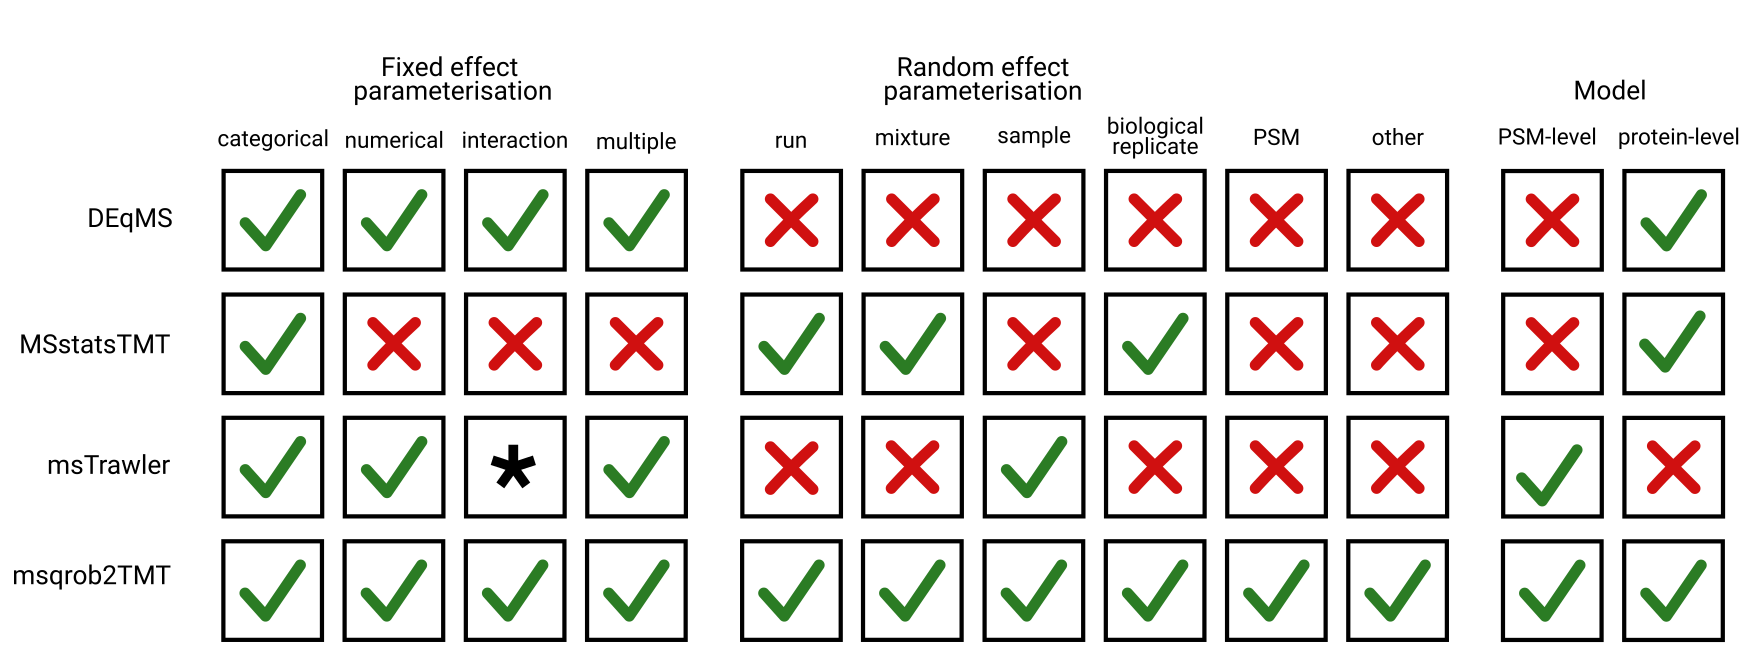
\includegraphics[width=1\textwidth,height=\textheight]{../figs/figure1.png}

}

\caption{\label{fig-model_overview}Overview of the tools considered in
this work and the model parameterisation they enable. Green tick marks
indicate that the method supports the specific model parameterisation.
Note, that ``other'' in the random effect parameterisation refers to
other random effects implied by the design, e.g.~in studies with
longitudinal or clustered designs. (*) msTrawler can only account for
interactions between a factor and a continuous time trend.}

\end{figure}%

\subsection{MSstatsTMT Spike-in Study}

In this study, 40 UPS1 proteins were spiked into a HeLa protein
background at four different concentrations. Each spike-in concentration
was multiplexed twice within a 10-plex TMT mixture, accompanied by two
reference channels. A total of five 10-plex TMT mixtures were prepared,
and each mixture was analysed in technical triplicate on the mass
spectrometer. Therefore, the ground truth is known: only the spike-in
UPS proteins are DA.

Note, that DEqMS cannot account for the hierarchical correlation
structure inherent in labelled experiments with multiple runs. While it
can correctly infer FCs when all conditions are present in each run by
introducing a block factor, it cannot adequately handle technical
repeats. Furthermore, it was also unclear how to account for technical
repeats from msTrawler's documentation. Consequently, in the main
manuscript, we assess the performance of the different methods using
only one technical repeat per mixture. Results for the full study,
including the analysis with multiple technical repeats, are provided in
the Supplementary Information.

In Figure~\ref{fig-WorkflowComparisons} A, we compare the performance of
the different methods using True Positive Rate (TPR) and False Discovery
Proportion (FDP) curves. The TPR represents the fraction of spiked UPS
proteins reported as DA, while the FDP reflects the proportion of HeLa
proteins among the total number of DA proteins returned. Our msqrob2TMT
workflows clearly outperform the state-of-the-art methods. Indeed, they
have a much higher sensitivity (TPR) at the same FDP level.

\begin{figure}[H]

\centering{

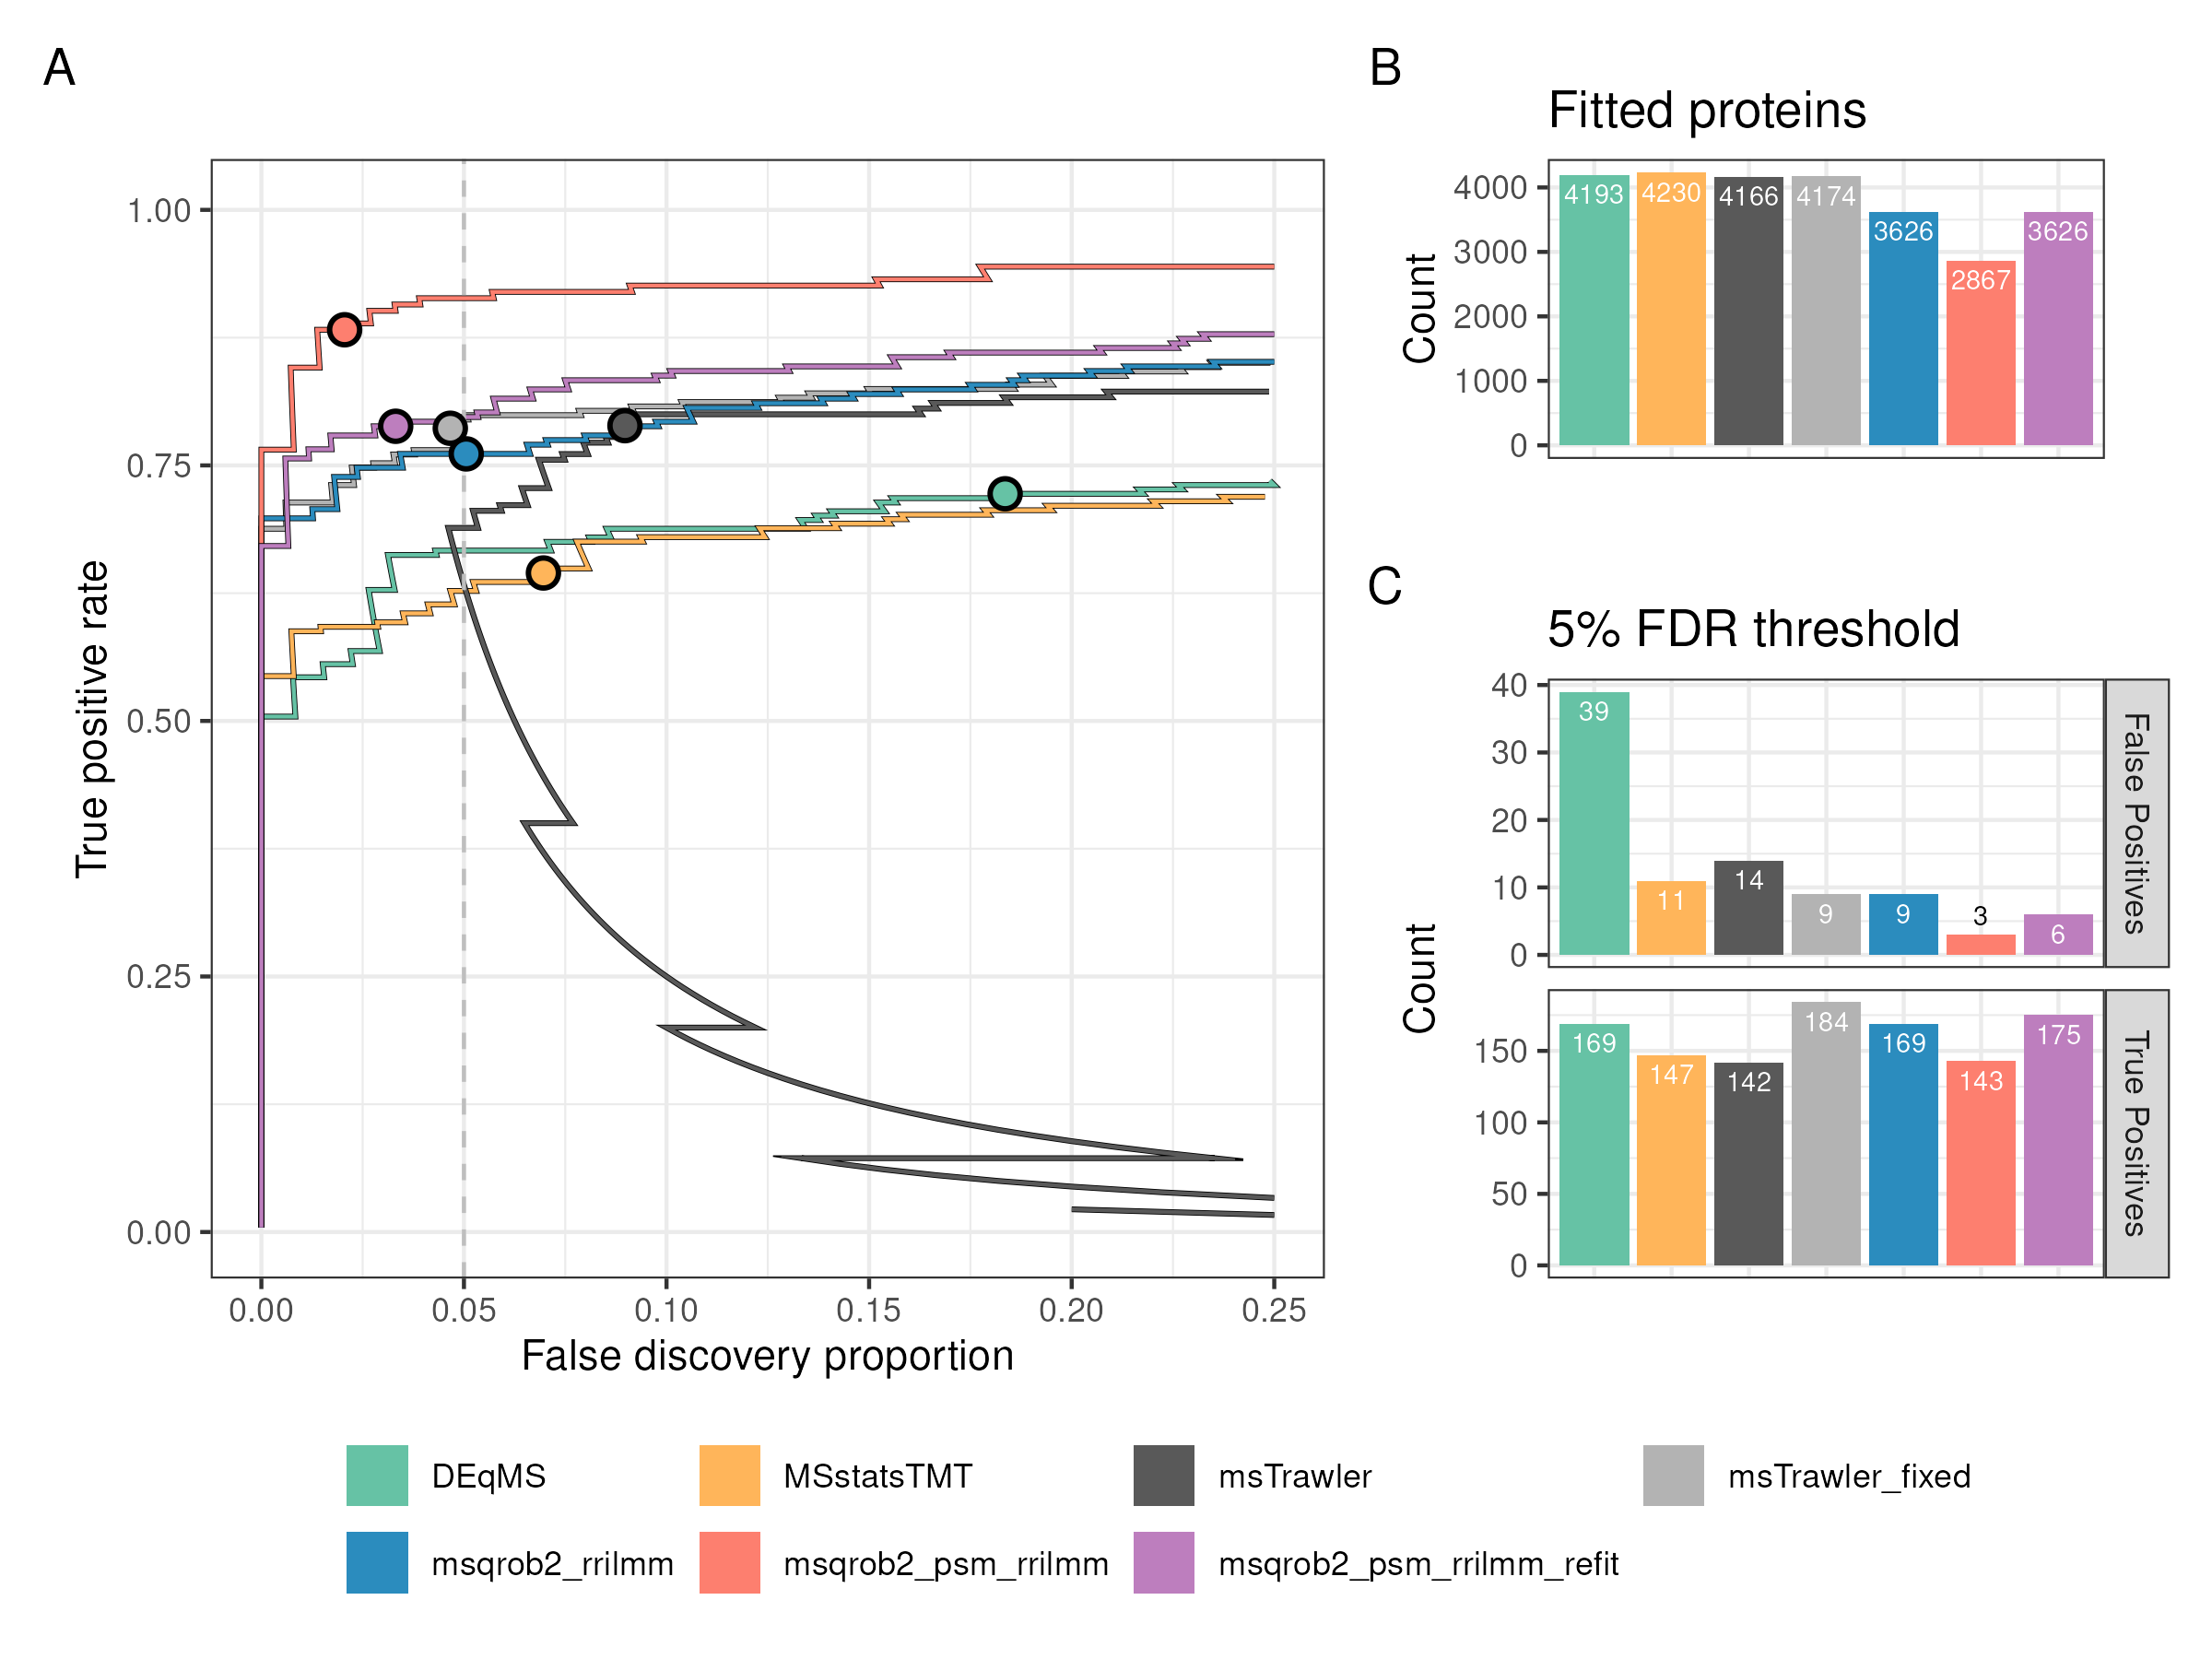
\includegraphics[width=1\textwidth,height=\textheight]{../figs/figure2.png}

}

\caption{\label{fig-WorkflowComparisons}Performance in the MSstatsTMT
spike-in study. Panel A: True positive rate (TPR) - false discovery
proportion (FDP) plots for DEqMS, MSstatsTMT, msTrawler and msqrob2TMT
workflows. Note, that the import function of msTrawler did not properly
import the data. So we also provide results for msTrawler with a
refactored import function, referred to as msTrawler~fixed. The combined
performance over all the dilution comparisons is shown. Dots indicate
the TPR and FDP obtained at the 5\% FDR threshold. Panel B: Number of
fitted proteins for each workflow. Panel C: Number of true and false
positives over all the comparisons.}

\end{figure}%

However, it is important to note that the different methods return
results for varying numbers of proteins, as shown in
Figure~\ref{fig-WorkflowComparisons} B. In particular, our novel
msqrob2-based workflows tend to report fewer proteins. To ensure a fair
comparison, we also present TPR-FDP curves based on all ground truth DA
proteins (all fourty spike-in UPS1 proteins) as the maximum number of TP
that can be reported for each comparison (Supplementary
Figure~\ref{fig-WorkflowComparisonsFull} B), as well as plots for the
common subset of proteins returned by all methods (Supplementary
Figure~\ref{fig-WorkflowComparisonsFull} C). Notably, Supplementary
Figure~\ref{fig-WorkflowComparisonsFull} B presents a different picture:
here, the PSM-level method msqrob2\_psm\_rrilmm shows significantly
lower sensitivity than the summarisation-based approaches. Specifically,
msqrob2\_psm\_rrilmm only returns models for 27 UPS proteins. This is
due to msqrob2\_psm\_rrilmm being unable to fit models for many proteins
because of missing data and/or due to one-hit-wonder proteins i.e.,
those for which only one peptide ion is observed. Indeed, for
one-hit-wonder proteins, msqrob2 cannot fit the random sample-level
effect and returns an error. To address this, we developed a refit
function that can automatically refit PSM-level models for
one-hit-wonders in our msqrob2\_psm\_rrilmm\_refit workflow. This
adaptation restores top performance when calculating the TPR based on
all 40 spike-in UPS proteins that are known to be DA in each comparison.
However, it should be noted that msqrob2\_psm\_rrilmm\_refit results in
a decrease in sensitivity compared to msqrob2\_psm\_rrilmm when TPR-FDP
curves are based solely on the proteins returned by each method
(Figure~\ref{fig-WorkflowComparisons} A), indicating that accounting for
one-hit-wonders leads to a faster accumulation of false positives among
the top-ranked proteins.

Interestingly, msTrawler, msqrob2\_psm\_rrilmm, and
msqrob2\_psm\_rrilmm\_refit show very similar performance when the
analysis is based on the common proteins returned by all methods, with
msqrob2\_rrilmm following closely behind (Supplementary
Figure~\ref{fig-WorkflowComparisonsFull} C). These results are
consistent with findings from label-free proteomics literature, where
PSM-level methods typically outperform summarisation-based workflows
(e.g., (Sticker et al. 2020)). Remarkably, msTrawler exhibited a
performance boost as compared to that in Supplementary
Figure~\ref{fig-WorkflowComparisonsFull} panels A and B, which probed us
to closely examine its top-ranked false positives. They appeared to be
spike-in proteins that were incorrectly labelled, which we could trace
back to the msTrawler import function that failed to read-in the data
correctly. Upon refactoring the lengthy msTrawler import function, which
is referred to as msTrawler\_fixed, the performance becomes on par with
msqrob2\_psm\_rrilmm\_refit.

These findings are further corroborated by the results at the 5\% FDR
level, shown in Figure~\ref{fig-WorkflowComparisons} C. All msqrob2
workflows demonstrate high sensitivity and low FDP. Specifically, they
recover between 143 - 175
\textcolor{red}{DA hits (true positives, TP) for} spike-in UPS proteins
\sout{as DA (true positives, TP)}\textcolor{red}{across all 6 pairwise comparisons}
while only reporting between 3 - 9 false positives (FP) for HeLa
proteins. As a result, their FDP ranges between 2.1\% - 5.1\%,
suggesting appropriate FDR control at the 5\% level. The default
msTrawler workflow, however, was only able to recover 142 TP and
reported 14 FP, leading to an FDP of 9\%. With our refactored import
function this improved to 184 TP, 9 FP and an FDP of 4.7\%. The
summarisation-based workflows DEqMS and MSstatsTMT, reported 169 and 147
TP, respectively, with 39 and 11 FP, resulting in FDPs of 18.8\% and
7\%, respectively, suggesting improper FDR control by DEqMS.

More detailed comparisons are available in Supplementary
Figure~\ref{fig-WorkflowComparisonsSeparateA}-\ref{fig-WorkflowComparisonsSeparateC},
which display TPR-FDP curves for individual pairwise comparisons of the
spike-in conditions. These figures highlight that the observed
performance improvements of our msqrob2 workflows are particularly
pronounced for more challenging comparisons involving low FCs (e.g.,
spike-in concentrations 0.667--0.5 and 1--0.667). In Supplementary
Figure~\ref{fig-WorkflowComparisonsTechreps}, we present results for the
full dataset, incorporating all technical repeats. While the results for
MSstatsTMT and our novel msqrob2TMT workflows are consistent with those
obtained from a single replicate, the difference in performance is
somewhat reduced when considering all technical repeats. It is worth
noting that only MSstatsTMT and our msqrob2 workflows can appropriately
analyse the full dataset, as DEqMS is unable to introduce random
effects, and it is unclear in msTrawler's documentation how to address
technical repeats.

In Figure~\ref{fig-fold_change_spike} we evaluate the \(\log_2\) FC
estimates. Figure~\ref{fig-fold_change_spike} A shows that the estimated
\(\log_2\) FC for non-spiked proteins is unbiased across all methods.
Interestingly, the variability of the estimates for the msqrob2TMT
workflows with ridge regularisation is lower. Note, that in comparison
0.667 - 0.5 and 1 - 0.125, there are extreme \(\log_2\) FC estimates of
-4.82 and -8.25, respectively, for the msTrawler workflow that are not
shown in the plots. Figure~\ref{fig-fold_change_spike} B demonstrates
that the \(\log_2\) FC for spike-in proteins are generally
underestimated by all methods. This is consistent with prior reports in
the literature and likely due to interference from co-fragmentation of
peptide ions, which causes the \(\log_2\) FC between reporter ions to be
underestimated (Savitski et al. 2011; Ow et al. 2009). We observe that
the underestimation becomes more pronounced as the \(\log_2\) FC between
conditions increases. The variability of the \(\log_2\) FC estimates for
the spiked UPS proteins is similar across all methods. This clearly
illustrates the benefit of the ridge regularisation in our msqrob2TMT
workflows as it affects only the \(\log_2\) FC estimates for non-DA
proteins while leaving those for DA proteins largely unchanged.

\begin{figure}[H]

\centering{

\includegraphics[width=1\textwidth,height=\textheight]{../figs/figure3.png}

}

\caption{\label{fig-fold_change_spike}Boxplots showing the log2 FC
distributions for the spike-in and non-spike-in proteins, focusing on
two comparisons with the highest and lowest difference in spike-in
concentrations. Fold changes are estimated by DEqMS, msqrob2TMT,
MSstatsTMT, and msTrawler workflows. The grey dotted line is the true
log2 FC for the comparison. Panel A: non spike-in proteins (HeLa); Panel
B: spike-in proteins (UPS).}

\end{figure}%

Finally, Supplementary Figure~\ref{fig-spikein1_pvalue_dist_nondiff}
shows that MSstatsTMT, msTrawler, and our msqrob2TMT workflows all
produce fairly uniform p-value distributions for non-spike-in proteins.
DEqMS, however, shows a slight inflation at low p-values. The ridge
regression p-values are slightly over-conservative with a notable spike
at p-values equal to 1, due to the shrinkage of FCs for non-spike-in
proteins.

\subsubsection{Impact of Robust Ridge Regression, Imputation and Reference Normalisation}

A unique feature of the msqrob2TMT workflows is the regularisation of
parameter estimation through robust M-estimation and ridge penalisation.
In Figure~\ref{fig-rrilmmComparisons}, we evaluate the impact of robust
ridge regression on performance within both protein-level and PSM-level
models. The results indicate a modest improvement in performance when
either robust M-estimation or ridge penalisation is applied
individually. However, the combination of robust M-estimation and ridge
penalisation yields the most substantial performance gain.

\begin{figure}[H]

\centering{

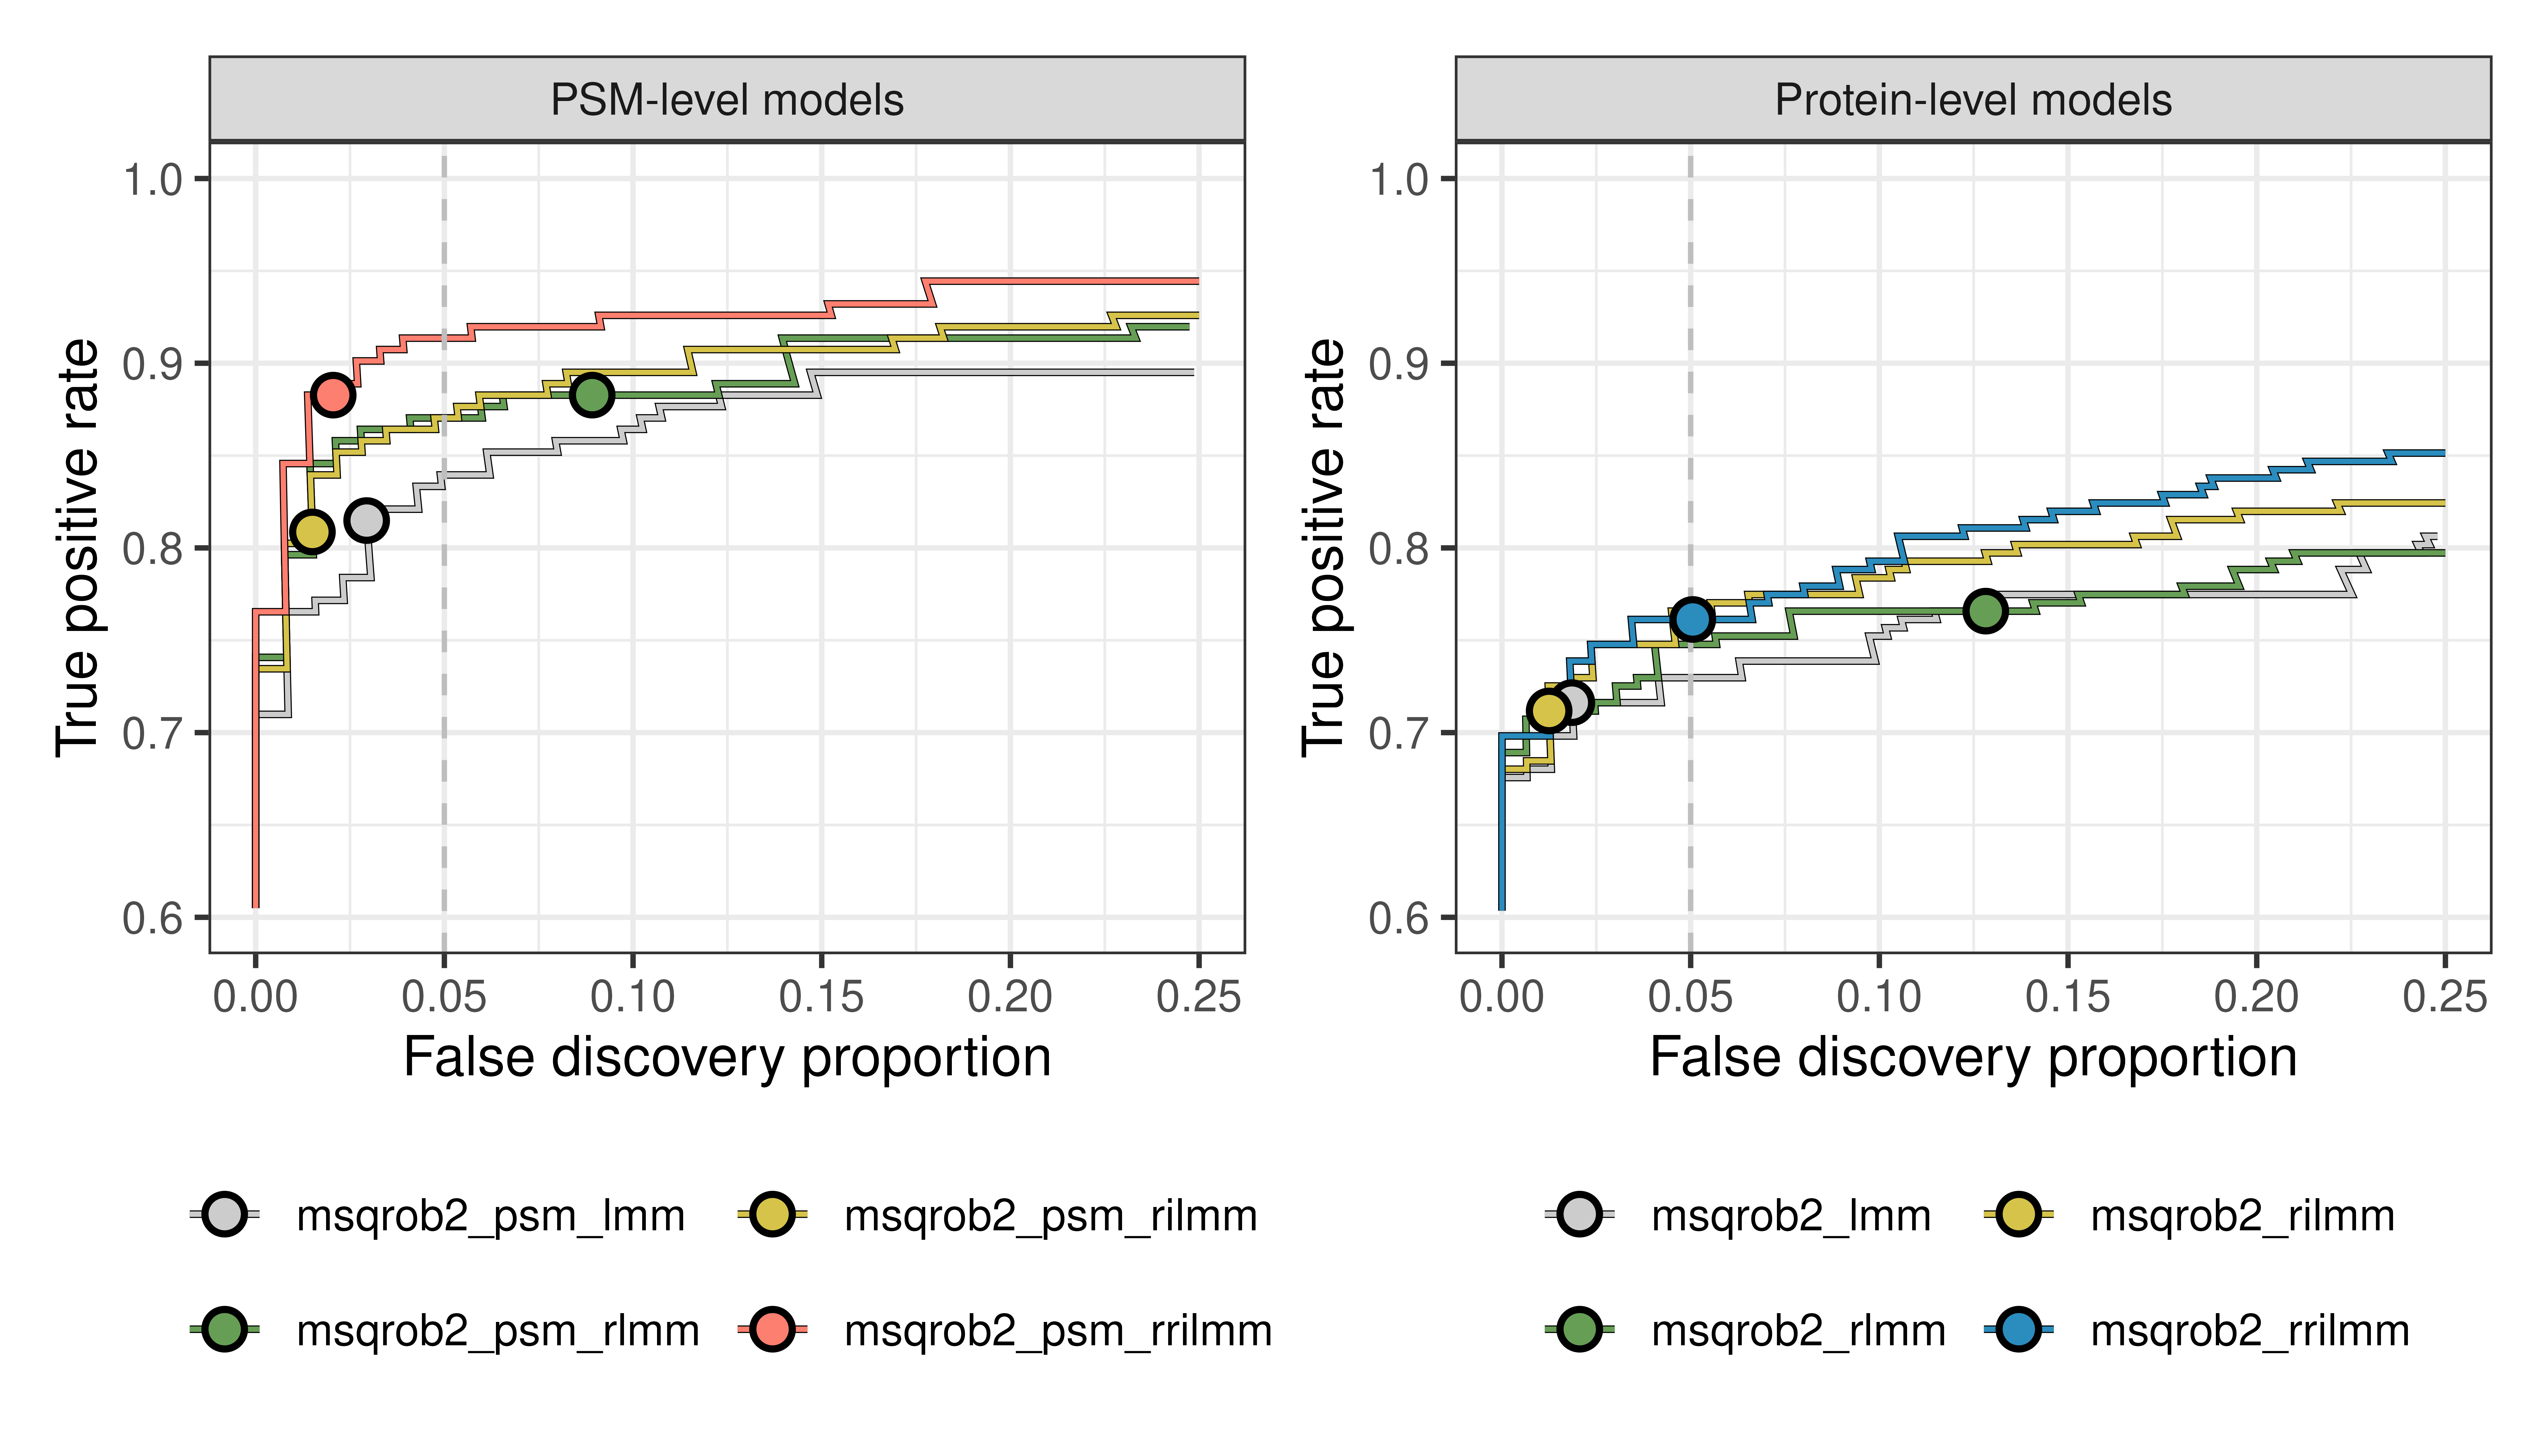
\includegraphics[width=1\textwidth,height=\textheight]{../figs/figure4.png}

}

\caption{\label{fig-rrilmmComparisons}True positive rate (TPR) - false
discovery proportion (FDP) plots showing the effect of robust
M-estimation and ridge regression on the performance of the msqrob2TMT
protein-level (panel A) and PSM-level workflows (panel B). Combined
performance over all comparisons is shown. Differential abundance is
inferred with msqrob2TMT with a vanilla linear mixed model (lmm), a
linear mixed model fitted via robust M-estimation (rlmm), ridge
regression (rilmm), or robust M-estimation and ridge regression
(rrilmm). Dots indicate the TPR and FDP obtained at the 5\% FDR
threshold.}

\end{figure}%

Note, that the msqrob2TMT workflow also differs from MSstatsTMT in its
preprocessing methodology. Specifically, MSstatsTMT, by default, imputes
missing values and employs reference channels for additional
normalisation. In Supplementary
Figure~\ref{fig-WorkflowComparisonsPreprocessing}, we evaluate the
integration of MSstatsTMT preprocessing with msqrob2TMT model fitting.
The findings reveal that imputation and reference channel normalisation
do not provide additional benefit in the context of this spike-in study.
Interestingly, a performance improvement is again observed when robust
M-estimation and ridge penalisation are applied.

\subsection{msTrawler Multibatch Benchmarking Study}

The msTrawler multibatch benchmarking study has a more complex design
comprising six TMTpro 18-plex batches, where two channels serve as
reference channels. One reference channel is derived from a single
batch, while the other reference channel includes data from all batches.
Yeast proteins cultured on different media were spiked in a background
of mouse proteins. The spike-in dilution ratios range from 1, 2, 3, 5,
11, 14, 18, 20, 24, 28, up to 32. Hence, the ground truth is known: only
the yeast proteins are DA. A correct data analysis requires modelling of
the spike-in condition, while blocking on culture media and accounting
for run-to-run variability. Note that this is not possible for
MSstatsTMT as users can only specify a single factor to model the
variability induced by the experimental design. Consequently,
incorporating MSstatsTMT would not provide a fair comparison and has
therefore been omitted from the results included in the main text.

It is important to note that the peculiar design of the experiment
implies unconventional preprocessing steps. Specifically, there is a
much higher number of DA yeast proteins, 1102 proteins, compared to
non-DA mouse proteins, 287 proteins, which violates the typical
assumptions of normalisation. Hence, we followed the bespoke
normalisation approach specifically devised for this dataset in the
msTrawler paper (O'Brien et al. 2024). In particular, the authors based
their normalisation on mouse proteins with low standard deviation,
i.e.~non-DA proteins that were consistently detected. Note that this
approach is not possible with real experimental data, where non-DA
proteins are typically unknown. For a fair comparison, we opted to apply
this bespoke preprocessing pipeline prior to conducting DA analysis with
DEqMS and our novel msqrob2TMT workflows.

In Figure~\ref{fig-WorkflowComparisonsSpikein2}, we compare the
performance of our msqrob2TMT workflows with the msTrawler and DEqMS
workflows across all dilution comparisons. The TPR-FDP plot in
Figure~\ref{fig-WorkflowComparisonsSpikein2} A demonstrates that
msqrob2\_psm\_rrilmm is again the top performer followed by the
msqrob2\_rrilmm and msqrob2\_psm\_rrilmm\_refit methods, which are on
par and outperform both msTrawler and DEqMS that exhibit lower
sensitivity. However, in Figure~\ref{fig-WorkflowComparisonsSpikein2} B,
a significant difference is observed in the number of proteins assessed
by each workflow. Notably, msqrob2\_psm\_rrilmm again reports fewer
results due fit errors for proteins with a lot of missing data and
one-hit wonder proteins. Nevertheless, following the refit that allows
for one-hit wonders, the number of proteins reported by msqrob2
increases by 47.8\%, indicating a very large number of one-hit-wonder
proteins. A substantial difference is also observed in the number of
false positives returned at the 5\% FDR threshold by each workflow
(Figure~\ref{fig-WorkflowComparisonsSpikein2} C). Specifically, DEqMS
and msTrawler report 387 and 676 false positives respectively, whereas
the msqrob2TMT workflows only return between 11 - 36 false positives at
the same 5\% FDR threshold. Notably, the protein-level msqrob2\_rrilmm
and msqrob2\_psm\_rrilmm\_refit still report about 4500 TPs more than
DEqMS. Lastly, all workflows exhibit an FDP below 5\%, which is not
unexpected, given that only 20.7\% of the proteins assessed are non-DA.
Indeed, the default Benjamini-Hochberg False Discovery Rate (BH-FDR)
method implicitly assumes the fraction of non-DA features to be 1 so as
to provide a conservative estimate of the expected proportion of false
positives in the list of significant features it returns (Efron et al.
2001), which is particularly conservative for this dataset with an
artificially high number of DA proteins.

\begin{figure}[H]

\centering{

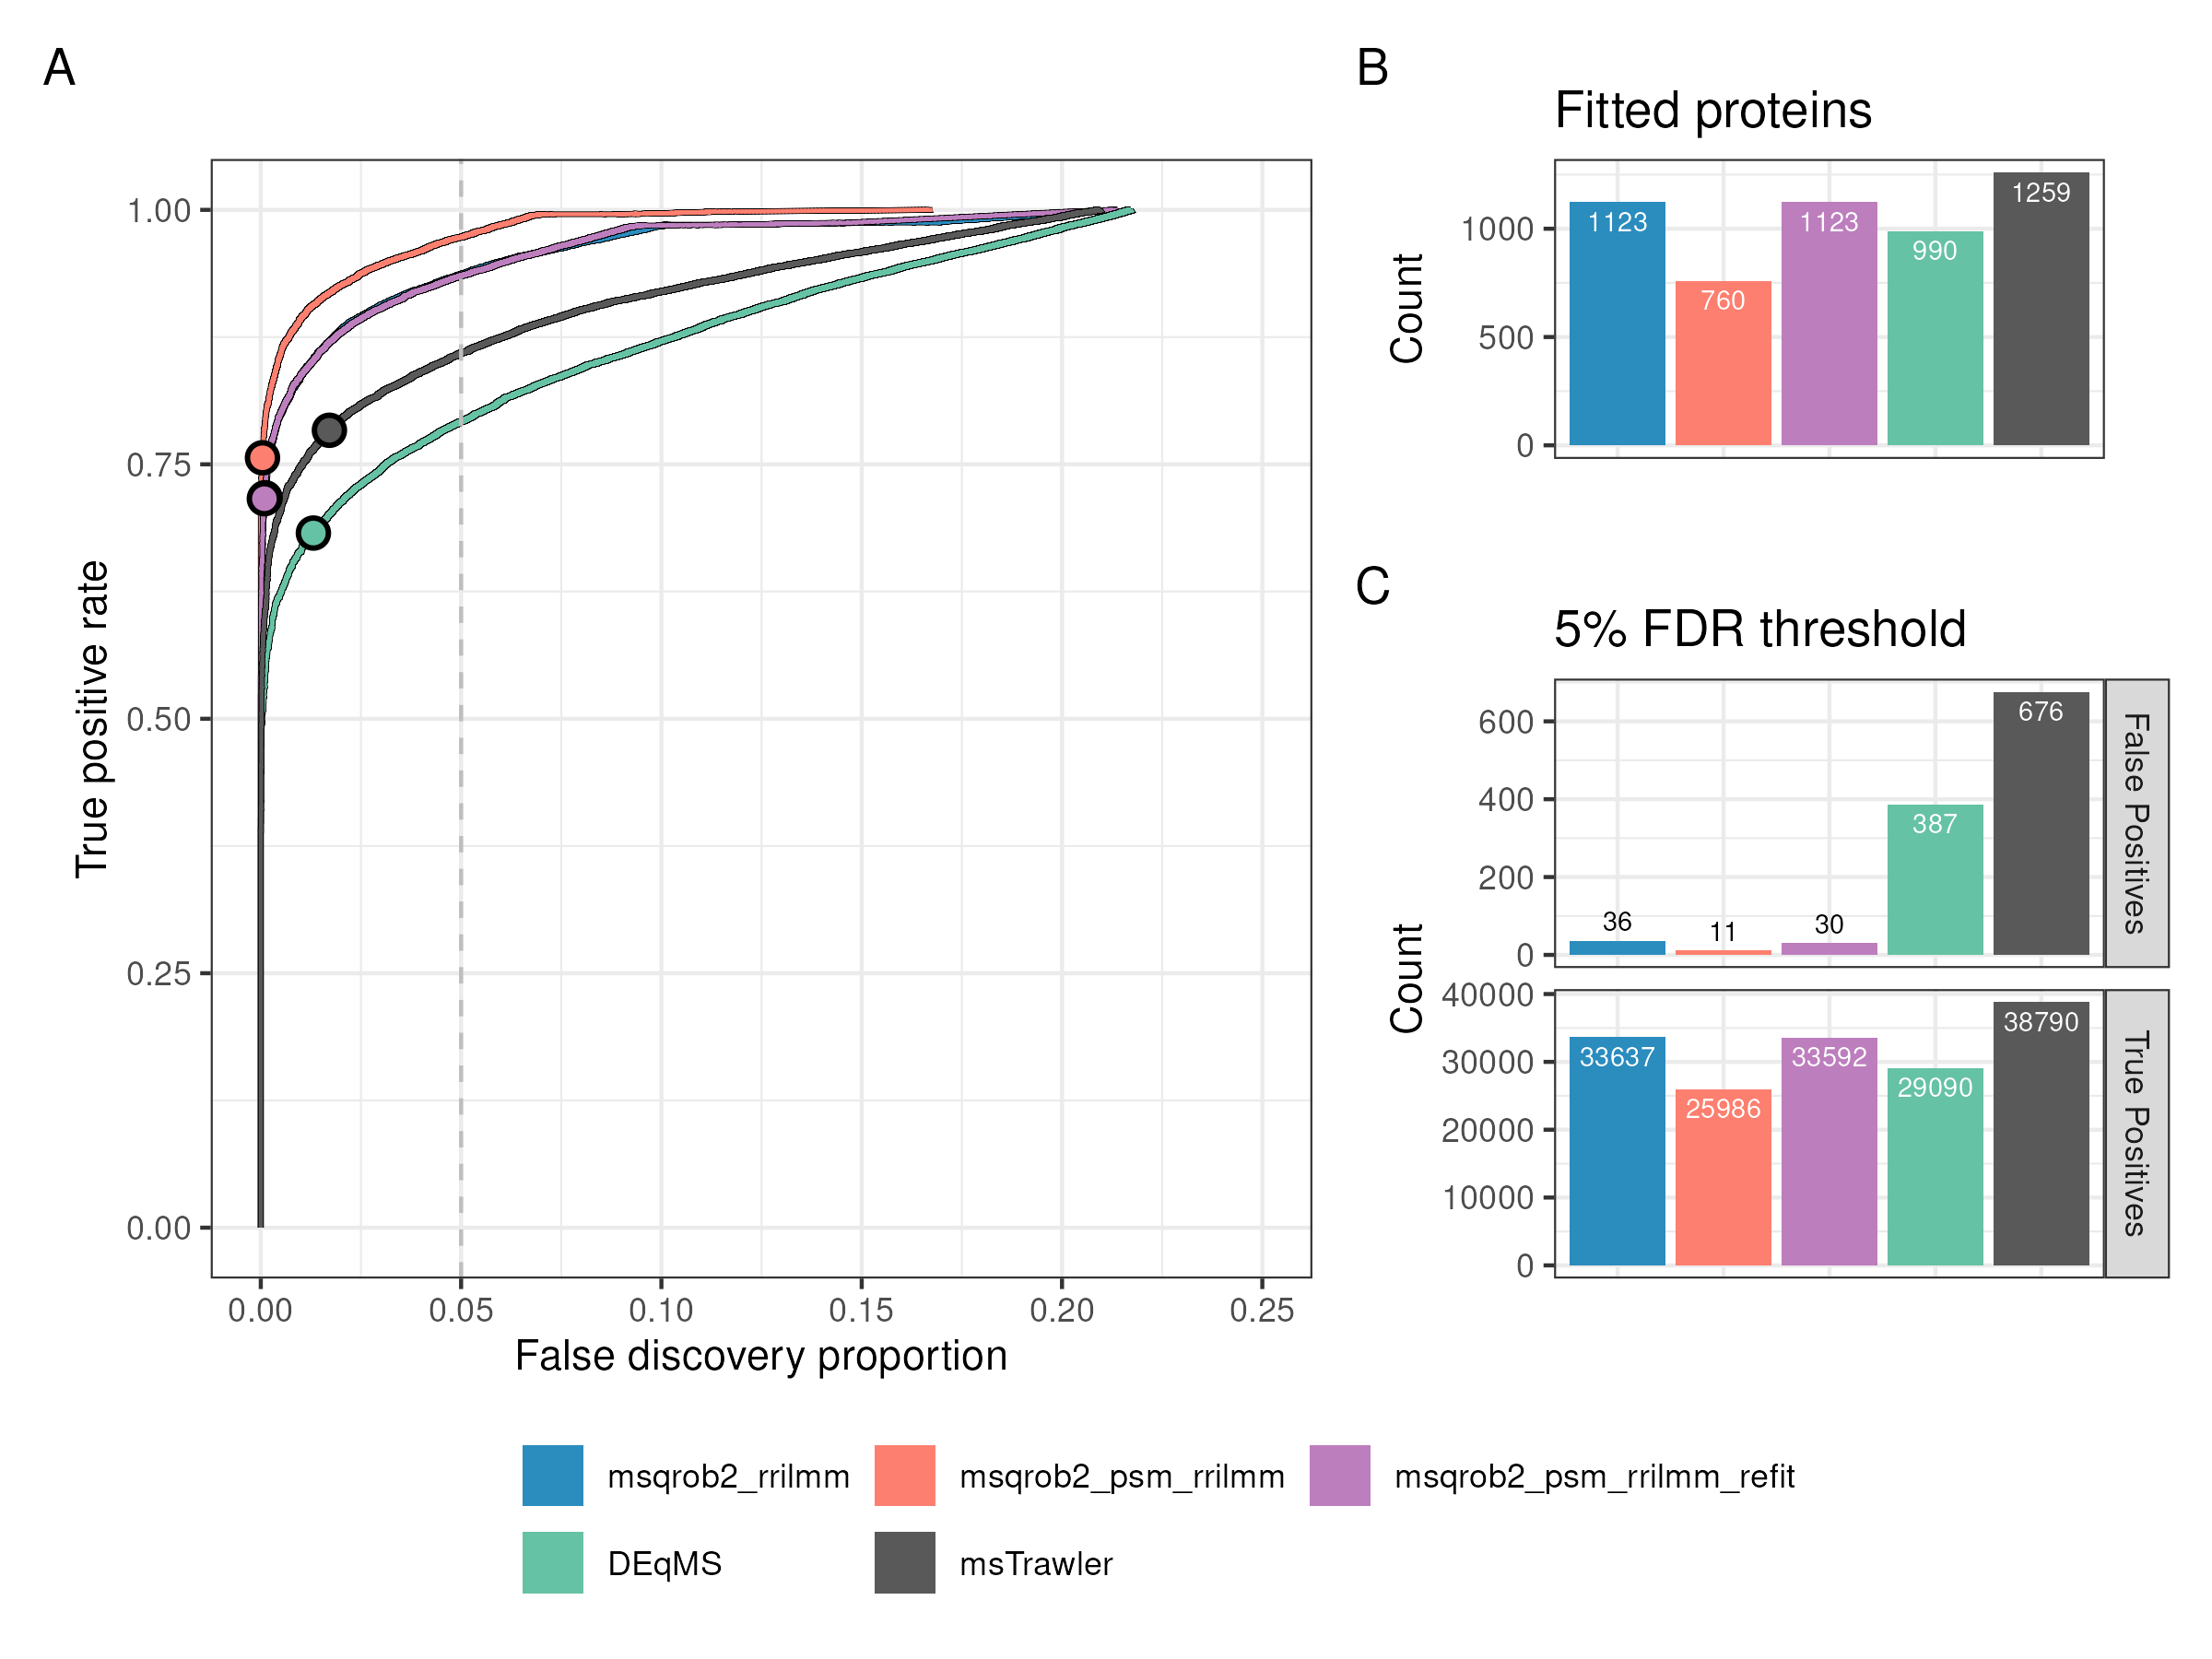
\includegraphics[width=1\textwidth,height=\textheight]{../figs/figure5.png}

}

\caption{\label{fig-WorkflowComparisonsSpikein2}Performance in the
msTrawler Multibatch Benchmarking Study. Panel A: True positive rate
(TPR) - false discovery proportion (FDP) plots for DEqMS, msTrawler, and
msqrob2TMT workflows. Combined performance over all comparisons is
shown. Dots indicate the TPR and FDP obtained at the 5\% FDR threshold.
Note, that the performance of msqrob2\_rrilmm and
msqrob2\_psm\_rrillm\_refit are on par, so their TPR-FDP curves almost
coincide. Panel B: Number of fitted proteins for each workflow. Panel C:
Number of true and false positives over all comparisons.}

\end{figure}%

For a fair comparison, we also report TPR-FDP curves using all ground
truth DA proteins as the maximum number of TP that can be reported for
each comparison (Supplementary
Figure~\ref{fig-WorkflowComparisonsSpikein2ALL} B) as well as those
based on the common subset of proteins assessed by all workflows
(Supplementary Figure~\ref{fig-WorkflowComparisonsSpikein2ALL} C). In
Supplementary Figure~\ref{fig-WorkflowComparisonsSpikein2ALL} B, we
observe a large decrease in performance for PSM-level method
msqrob2\_psm\_rrilmm, which is due to the vast number of one-hit-wonder
yeast proteins. However, after refitting, msqrob2\_psm\_rrilmm\_refit
recovers performance comparable to that of our msqrob2\_rrilmm workflow,
which outperform msTrawler irrespectively of the set of ground truth DA
proteins that is used to calculate the TPR (Supplementary
Figure~\ref{fig-WorkflowComparisonsSpikein2ALL} A-C). Note, however,
that the methods also differ in terms of their preprocessing.
Specifically, msTrawler employs imputation and additional filtering. In
Supplementary Figure~\ref{fig-WorkflowComparisonsPreprocessingSpikein2},
we therefore present results for msqrob2TMT models applied on
msTrawler's preprocessed data, which demonstrates a further increased
performance. This finding confirms the superior model fitting of our
msqrob2TMT workflows compared to msTrawler.

To illustrate the importance of msqrob2TMT's flexibility in
accommodating arbitrarily complex experimental designs, we included
results in Supplementary Figure~\ref{fig-WorkflowComparisonsSpikein2ALL}
that MSstatsTMT users would obtain if they omitted the blocking effect
in their analysis. As expected, excluding this blocking factor leads to
a significant reduction in performance.

In Figure~\ref{fig-fold_change_spike2}, we evaluate the \(\log_2\)FC
estimates for non-DA mouse proteins and DA spike-in yeast proteins.
Notably, the variability in \(\log_2\)FC estimates for non-DA mouse
proteins is markedly lower and closer to zero for the msqrob2TMT
workflows. Similar to Figure~\ref{fig-fold_change_spike}, \(\log_2\)FC
values for DA proteins are generally underestimated across all
workflows, with similar levels of variability observed. This again
highlights the beneficial property of our msqrob2TMT robust ridge
workflows in reducing variability for non-DA proteins, without affecting
these for truly DA proteins.

\begin{figure}[H]

\centering{

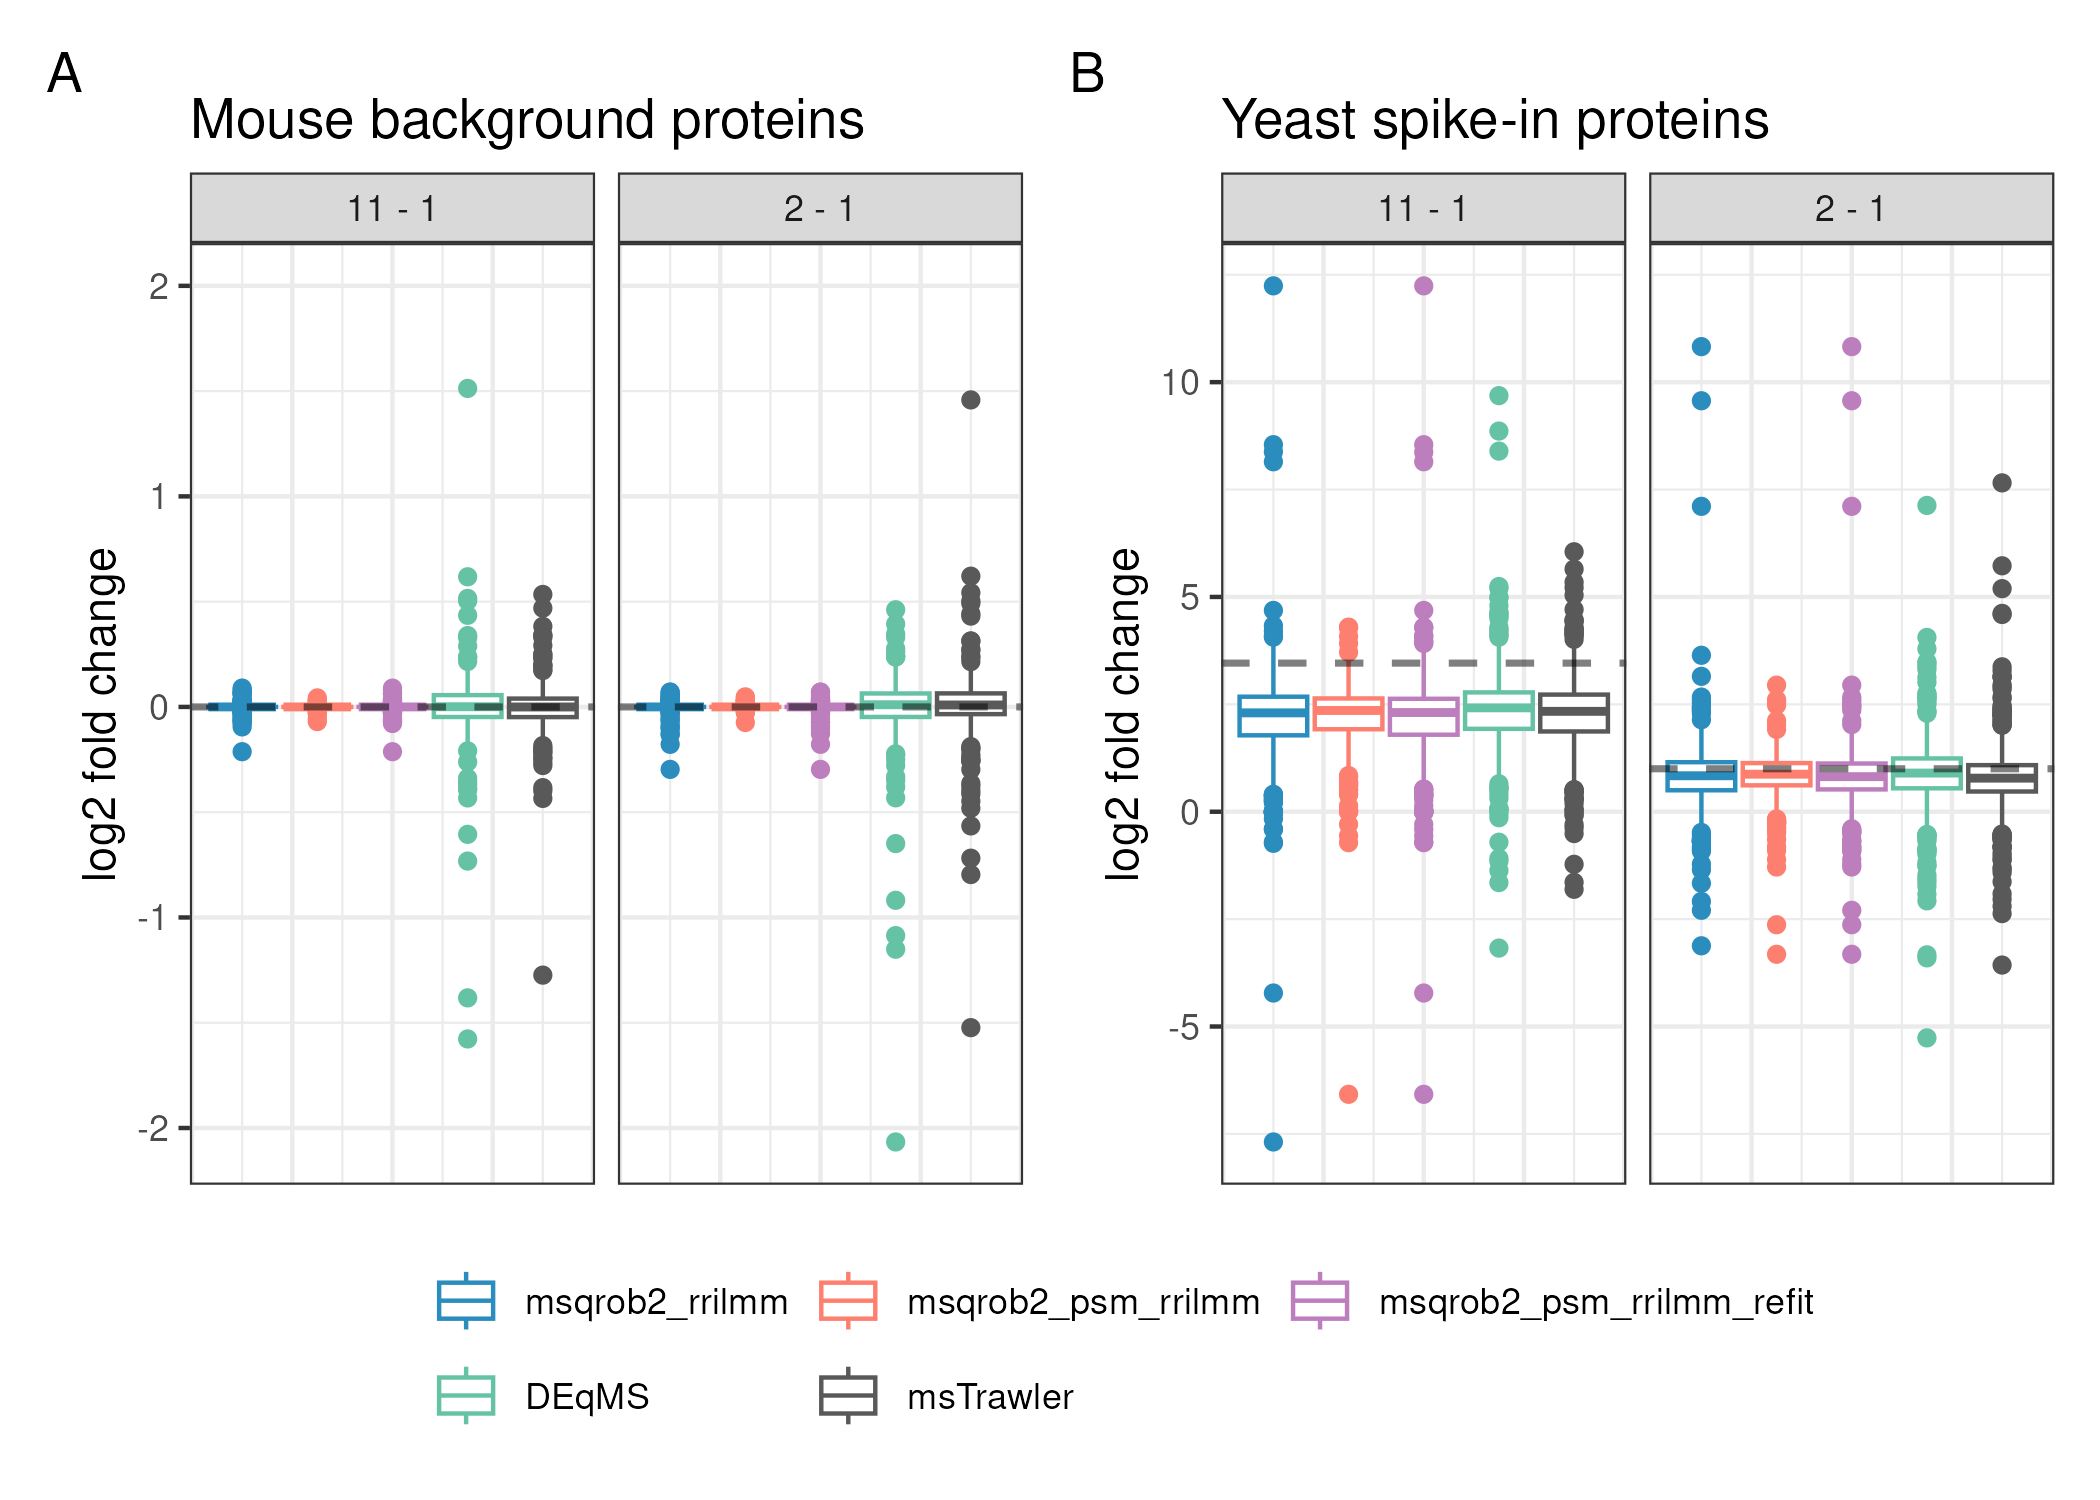
\includegraphics[width=1\textwidth,height=\textheight]{../figs/figure6.png}

}

\caption{\label{fig-fold_change_spike2}Boxplots showing the log2 FC
distributions for the spike-in proteins, focusing on two comparisons
with the highest and lowest difference in spike-in concentrations. Fold
changes are estimated by DEqMS, msqrob2TMT, and msTrawler workflows. The
grey dotted line is the true log2 FC for the comparison. Panel A:
non-spiked proteins (mouse); Panel B: spike-in proteins (yeast).}

\end{figure}%

Finally, Supplementary Figure~\ref{fig-spikein2_pvalue_dist_nondiff}
illustrates that both the msTrawler and msqrob2TMT workflows generate
relatively uniform p-value distributions for non-spike-in proteins. The
p-values derived from ridge regression are slightly over-conservative,
and due to the shrinkage of FCs for the non-spiked proteins, there is a
noticeable peak of p-values at 1. This histogram exhibits greater
variability compared to Supplementary
Figure~\ref{fig-spikein1_pvalue_dist_nondiff} likely due to the limited
number of non-DA mouse proteins in the dataset (287 proteins only).

\subsection{Mouse Study}

This study investigates the effect of the diet and duration on the
proteome of adipocyte cells. The mouse dataset involves mice that were
subjected to either a low-fat (LF) or a high-fat (HF) diet for varying
durations, also referred to as short or long period. Note, that
MSstatsTMT cannot accommodate for designs with multiple factors and/or
interactions. We therefore encode the treatment effect as a single
factor, with each level corresponding to a specific diet \(\times\)
duration combination. The primary research focus lies on the effect of
diet. Accordingly, we prioritise proteins using the following four
contrasts:

\begin{enumerate}
\def\labelenumi{\arabic{enumi}.}
\tightlist
\item
  DA between mice exposed to a HF vs LF diet after a short period,
  representing an early diet effect.
\item
  DA between mice exposed to a HF vs LF diet after a long period,
  representing a late diet effect.
\item
  DA between mice exposed to a HF vs LF averaged over the early and late
  period, representing an average diet effect.
\item
  DA between mice exposed to a HF vs LF diet differs between long and
  short period, representing the diet \(\times\) duration interaction
  effect.
\end{enumerate}

Note, that msTrawler will automatically generate output files for all
pairwise comparisons between each diet \(\times\) duration combination.
However, it does not allow users to define their contrasts of interest.
Consequently, the diet \(\times\) duration interaction and the average
diet effect cannot be inferred using msTrawler. Furthermore, attempts to
utilise msTrawler with multiple reference samples available per run were
unsuccessful, even when subsampling was applied. Additionally, we could
not address the correlation between fractions with the software, thereby
preventing us from addressing the hierarchical correlation structure
inherent to the dataset. Due to these limitations, msTrawler was
excluded from the analysis.

We also include two protein-level msqrob2TMT workflows. In the first
workflow, msqrob2tmt\_rrilmm, peptide ions are summarised to the
protein-level for each run, resulting in multiple protein abundance
values for each biological replicate i.e., one in every technical
fraction. In the second workflow, msqrob2tmt\_rrilmm\_mixture, we use
the MSstatsTMT approach and summarise peptide ions to the protein-level
over all technical fractions, resulting in a single protein abundance
value for every biological replicate.

\begin{table}[H]

\caption{\label{tbl-MouseStudyWorkflowComparison}Number of differential
proteins at 5\% FDR for the msqrob2 and MSstatsTMT workflows. The
proteins are prioritised using the following four contrasts: DA between
HF vs LF diet after short period (early), DA between HF vs LF diet after
long period (long), average DA between HF vs LF over the early and late
period (avg), and DA of HF vs LF diet differs between long period and
short period (int).}

\centering{

\fontsize{9.8pt}{11.7pt}\selectfont
\begin{tabular*}{\linewidth}{@{\extracolsep{\fill}}l|rrrr}
\toprule
 & \multicolumn{4}{c}{Comparison} \\ 
\cmidrule(lr){2-5}
 & early & late & avg & int \\ 
\midrule\addlinespace[2.5pt]
MSstatsTMT & 5 & 9 & 27 & 1 \\ 
msqrob2\_rrilmm\_mixture & 31 & 6 & 50 & 5 \\ 
msqrob2\_rrilmm & 80 & 21 & 119 & 7 \\ 
msqrob2\_psm\_rrilmm & 95 & 24 & 132 & 4 \\ 
msqrob2\_psm\_rrilmm\_refit & 98 & 29 & 145 & 6 \\ 
\bottomrule
\end{tabular*}

}

\end{table}%

Table~\ref{tbl-MouseStudyWorkflowComparison} summarises the number of DA
proteins identified as significant at the 5\% FDR-adjusted p-value
threshold by the various methods. First, the PSM-level workflows
(msqrob2\_psm\_rrilmm and msqrob2\_psm\_rrilmm\_refit) return more DA
proteins than protein-based workflows for three out the four contrasts
tested. Note, that the fourth contrast is the diet \(\times\) duration
for which few DA proteins were identified, irrespective of the method.
Indeed, high throughput omics studies are known to be under powered for
discovering interaction effects (Van den Berge et al. 2018). Second,
modelling the technical MS fraction (msqrob2\_psm\_rrilmm,
msqrob2\_psm\_rrilmm\_refit and msqrob2\_rrilmm) leads to a striking
increase of the number of DA proteins compared to the workflows that
summarise protein intensities over the technical fractions of a mixture
(MSstatsTMT, msqrob2\_rrilmm\_mixture). Third, more DA proteins are
found by our msqrob2TMT workflows compared to MSstatsTMT, even when
applying the same summarisation approach, i.e.~MSstatsTMT vs
msqrob2\_rrilmm\_mixture. Finally, allowing for one-hit-wonder proteins
when modelling the data at the PSM level (msqrob2\_psm\_rrilmm\_refit)
slightly increases the number of DA, making it the workflow that
identifies the most DA proteins. However, as the ground truth for DA
proteins in this experimental dataset is not available, we are unable to
affirm whether the reported proteins are truly DA.

The upset plots (Supplementary
Figures~\ref{fig-Upset-early}-\ref{fig-Upset-avg}) demonstrate that the
majority of the proteins identified by msqrob2\_rrilmm and
msqrob2\_rrilmm\_mixture are also prioritised by the PSM-level models
(msqrob2\_psm\_rrilmm and msqrob2\_psm\_rrilmm\_refit). Additionally,
most of the 5, and 27 DA proteins that were reported by MSstatsTMT for
the early and average diet contrasts, respectively, were also found
significant by other msqrob2TMT workflows. The few proteins uniquely
identified as DA by MSstatsTMT where either no longer significant for
our msqrob2TMT workflows after correcting for multiple testing i.e.,
four proteins in the late comparison, or could not be fitted due to
missingness i.e., two proteins in the late comparison and all five
proteins in the average comparison. Furthermore, proteins uniquely
reported by msqrob2\_rrilmm\_mixture again were no longer significant
for the other msqrob2TMT workflows after correcting for multiple testing
or could not be fitted due to missingness. Interestingly, the latter
proteins exhibited FCs similar to those detected by MSstatsTMT, although
their MSstatsTMT p-values were no longer significant after correcting
for multiple testing. Finally, proteins uniquely identified as DA by
msqrob2\_rrilmm or msqrob2\_psm\_rrilmm have FCs comparable to those
observed in other workflows. Again, the corresponding p-values in the
other methods were no longer significant upon correcting for multiple
testing.

We also conducted a over-representation analysis for the average diet
effect, as this comparison yielded the largest list of DA proteins
(Supplementary Figure Figure~\ref{fig-ora}). The over-representation
analysis can be performed against a background consisting of the entire
mouse proteome or restricted to the proteins identified in the study.
The latter approach is more convenient. Indeed, the proteins are
isolated from mouse adipose tissue, which is expected to result in an
over-representation of adipose tissue-specific proteins. Using this
restricted background, only seven metabolic pathways were found to be
significantly enriched with our msqrob2TMT PSM-level workflows, three of
which were also detected by our protein-level workflow msqrob2\_rrilmm.
However, no KEGG pathways were significantly enriched when employing the
two protein-level workflows that summarise peptide-ions across fractions
(MSstatsTMT and msqrob2\_rrilmm\_mixture). Hence, we also performed the
over-representation analysis against the entire mouse background
proteome to enable broader comparisons. With this approach, all our
novel msqrob2TMT workflows found multiple significantly enriched KEGG
pathways, again all related to metabolism, as opposed to MSstatTMT,
which did not pick up any enriched KEGG pathway.

Finally, we assessed the validity of the p-values through a mock
analysis. Specifically, we randomly assigned the samples of each diet
\(\times\) duration combination within a mixture to two mock conditions.
As none of the proteins exhibit DA between the mock conditions, the
corresponding p-values should follow a uniform distribution. The mock
analysis could only be conducted with our msqrob2TMT workflows, as it is
not feasible to analyse a two-factor design with additive effects using
MSstatsTMT. As shown in Supplementary Figure~\ref{fig-mouse-mock-pval},
the p-value distributions are uniform with a spike on 1. This pattern,
also observed in the spike-in study, again originates from shrinkage of
the model parameters towards zero. The results of the mock analysis
suggests that the additional proteins found to be significant with our
novel msqrob2TMT workflows are not driven by overly liberal asymptotic
inference.

\section{Discussion}

In this contribution, we introduced msqrob2TMT, a novel suite of
workflows within our msqrob2 universe, designed to perform differential
abundance (DA) analysis for labelled mass spectrometry (MS)-based
proteomics experiments. These workflows leverage the flexible robust
ridge regression framework of msqrob2 to enhance performance compared to
the state-of-the-art tools DEqMS, MSstatsTMT, and msTrawler that uses
standard linear (mixed) models.

With the release of msqrob2 version 1.14, we have unlocked full
compatibility with the lme4 R package for mixed models, enabling the
analysis of data from more complex experimental designs that require the
use of both feature-level and sample-level covariates. This advancement
allows our workflows to address the intricate hierarchical correlation
structure inherent to data from labelled MS experiments, facilitating
the analysis of datasets with arbitrarly complex layouts. This
capability is particularly critical for modelling data generated in
contemporary labelled proteomics experiments, as these utilise ever more
complex designs.

Our evaluations on two spike-in studies and a case study demonstrate
that none of the three state-of-the-art tools included in our
comparisons could provide valid inference across all of these datasets.
Notably, MSstatsTMT was unable to account for an additional block effect
associated to growth medium in the msTrawler Multibatch Benchmarking
Experiment, a limitation with far reaching implications for its
applicability in biomedical contexts. Indeed, the inability to adjust
for additional covariates and potential confounders undermines the
utility of MSstatsTMT in such settings. msTrawler and DEqMS, on the
other hand, could not accommodate the more complex correlation
structures of the MSstatsTMT spike-in study with technical repeats or
the multiple fractions in the mouse case study. Yet these experimental
setups are widely employed in the proteomics community, underscoring the
limitations of these tools in addressing such commonly encountered
experimental designs.

An additional drawback of msTrawler is its restriction on hypothesis
testing. Unlike msqrob2TMT, msTrawler automatically generates output
files for testing the slope of each additive covariate in the model as
well as for all pairwise comparisons between the levels of each factor
variable. However, it does not allow users to define custom hypotheses
of interest, such as interaction effects between factors or contrasts
like the average treatment effect of one factor when they are involved
in an interaction. This limitation diminishes its utility in
prioritising proteins of interest, as demonstrated in our mouse case
study, where assessing the average treatment effect enabled the
identification of the largest number of DA proteins.

Notably, msqrob2TMT not only improves over the state-of-the-art tools in
terms of its flexibility, but also demonstrates superior performance. In
our analysis of the MSstatsTMT spike-in and msTrawler's multibatch
benchmarking datasets, we showed that our novel msqrob2TMT workflows
outperform the existing methods in terms of sensitivity, specificity and
FDR control. These improvements underscore the importance of the
parameter estimation procedure in DA workflows. By extending the linear
mixed model to enhance robustness against outliers and improve
uncertainty estimation, msqrob2TMT achieves substantial performance
gains. The tools also differ in their preprocessing, specifically in
normalisation and imputation. Different sources of missingness occur,
which can lead to suboptimal results when the data are imputed under the
assumption of missingness by low abundance. The robust modelling in
msqrob2TMT, however, can safely omit imputation altogether. msqrob2TMT
is also modular, which provides its users with the flexibility to use
custom preprocessing steps, making it future-proof when novel and more
performant normalisation, summarisation, or imputation procedures become
available.

Another significant distinction between the msqrob2, MSstatsTMT, and
msTrawler packages lies in their approach to model fitting. MSstatsTMT
and msTrawler aim to fit as many proteins as possible by automating the
model fitting process. While this approach enhances ease of use, it can
result in fitting proteins from the same dataset using different
models---for instance, combining linear models with mixed models. This
practice may not always be appropriate for the analysis and can
introduce complexities in interpretation. Although it is possible to
retrieve the underlying models and evaluate their validity, standard
users may not be fully aware of these issues or the nuanced
interpretations they entail. In contrast, the msqrob2TMT workflows
prioritise transparency and reproducibility. Rather than automatically
reducing models when the user-specified model cannot be fitted,
msqrob2TMT explicitly reports a fit error. This approach allows the data
analyst to refit specific proteins with a more appropriate model,
ensuring greater consistency and interpretability. We developed a refit
function for this purpose and provide detailed guidance in our vignettes
(Supplementary Information) to support our users in adapting their
analysis to incorporate this feature.

Our analyses also highlight the critical need for robust benchmark
datasets in the field of proteomics. Both the MSstatsTMT spike-in
dataset and the msTrawler multibatch benchmarking study, while valuable,
have notable limitations. Specifically, all DA proteins in these
datasets are spike-in in the same direction, which puts a severe burden
on the conventional assumptions underlying normalisation procedures.
This can result in issues with channel normalisation, as other proteins
may become biased downwards due to ion suppression effects in samples
with high spike-in concentrations. In the msTrawler multibatch
benchmarking study, the authors had to develop a bespoke preprocessing
workflow tailored specifically to this dataset. Indeed, the data
contained up to five times more DA proteins than non-DA proteins and all
DA between spike-in conditions is in the same direction, which is highly
unrealistic. Notably, their normalisation method explicitly had to rely
on stably expressed, non-DA proteins, which are typically unknown in a
real experimental setting. Conversely, in the MSstatsTMT spike-in study,
both non-DA background HeLa UPS proteins as well as spike-in UPS
proteins are present. As the HeLa and UPS proteins differ in metabolic
labelling, one should be able to discriminate between the non-DA and DA
UPS proteins. When closely examining the PSM-level data provided by the
MSstatsTMT authors, however, we found spectra that match perfectly with
a DA pattern expected for spike-in proteins, whilst being tagged as HeLa
and vice versa. We therefore performed additional preprocessing steps to
exclude these ambiguous proteins. Nevertheless, it remains possible that
some spectra are still mislabelled. This mislabelling can lead to two
key issues: on the one hand, there may be an excess of perceived false
positives originating from spike-in proteins that were erroneously
tagged as background UPS proteins; on the other hand, there may be a
reduction in sensitivity. The inclusion of spectra from mislabelled
background UPS proteins diminishes the \(\log_2 FC\) estimates and
increases the standard errors, which can result in spike-in UPS proteins
not being identified as significant. When the analysis was conducted
without our additional preprocessing, more false positives were
observed. This as a result of background proteins that had not been
tagged as spike-in UPS proteins, but clearly exhibited a DA pattern
consistent with spike-in UPS proteins. After thoroughly examining these
two recent state-of-the-art spike-in studies, we urge the field to
progress by developing novel benchmark datasets that encompass more
complex DA patterns, where some proteins are upregulated while others
are downregulated within each spike-in condition.

Overall, we have demonstrated that our msqrob2TMT workflows offer
distinct advantages over state-of-the-art tools. They provide a more
sensitive and robust approach, while providing good false discovery rate
control. Furthermore, these workflows offer the flexibility to infer DA
from data derived from experiments with arbitrarily complex designs, a
crucial feature for analysing large-scale MS-based proteomics datasets
that are increasingly prevalent. Our modular implementation gives our
users full flexibility with respect to the choice of search engine,
preprocessing steps, and the research hypotheses it can address, while
delivering a comprehensive, transparent, and reproducible workflow that
spans the entire differential proteomics data analysis.

\section{Data Availability}

All analyses presented in this paper can be reproduced using msqrob2
version 1.14.1 from Bioconductor release 3.20, available at
\url{https://doi.org/doi:10.18129/B9.bioc.msqrob2}, and the scripts on
our companion GitHub page:
\url{https://github.com/statOmics/msqrob2tmt_paper}. We also provide a
Docker image containing the computational setup used to generate the
results:
\url{https://hub.docker.com/repository/docker/cvanderaa/msqrob2tmt}. To
assist users in building their own msqrob2TMT workflows and interpreting
the output, we have included two vignettes in the Supporting
Information. The data from the MSstatsTMT spike-in study, the msTrawler
multibatch benchmarking study and the mouse case study are available in
the PRIDE repositories under PXD0015258, PXD036799, and PXD005953,
respectively. For the reproducibility of results, the data for
PXD0015258, PXD036799, and PXD005953 were downloaded from MassIVE
(RMSV000000265), Google Drive
(\url{https://console.cloud.google.com/storage/browser/mstrawler_paper}),
and MassIVE (RMSV000000264), respectively, and timestamped by creating a
Zenodo repository: \url{https://zenodo.org/records/14767905}.

\section{Funding}

This research was funded by the Research Foundation Flanders (FWO) as
project funding awarded to L. M. (G010023N, G028821N) and L. C.
(G062219N) and as WOG (W005325N) to L. M. and L. C., funding from the
European Union's Horizon Europe Programme (101080544 and 101191739), and
funding from a Ghent University Concerted Research Action to L. M.
{[}BOF21/GOA/033{]} and L. C. {[}BOF20/GOA/023{]}.

\section{References}

\phantomsection\label{refs}
\begin{CSLReferences}{1}{0}
\bibitem[\citeproctext]{ref-Brenes2019}
Brenes, Alejandro, Jens Hukelmann, Dalila Bensaddek, and Angus I.
Lamond. 2019. {``Multibatch {TMT} Reveals False Positives, Batch Effects
and Missing Values.''} \emph{Molecular \& Cellular Proteomics} 18 (10):
1967--80. \url{https://doi.org/10.1074/mcp.ra119.001472}.

\bibitem[\citeproctext]{ref-efron2001localfdr}
Efron, Bradley, Robert Tibshirani, John D. Storey, and Virginia Tusher.
2001. {``Empirical {Bayes} Analysis of a Microarray Experiment.''}
\emph{Journal of the American Statistical Association} 96 (456):
1151--60.

\bibitem[\citeproctext]{ref-Qfeatures2022}
Gatto, Laurent, and Christophe Vanderaa. 2022. \emph{QFeatures:
Quantitative Features for Mass Spectrometry Data}.
\url{https://github.com/RforMassSpectrometry/QFeatures}.

\bibitem[\citeproctext]{ref-Goeminne2020}
Goeminne, Ludger J. E., Adriaan Sticker, Lennart Martens, Kris Gevaert,
and Lieven Clement. 2020. {``{MSqRob} Takes the Missing Hurdle: Uniting
Intensity- and Count-Based Proteomics.''} \emph{Analytical Chemistry} 92
(9): 6278--87. \url{https://doi.org/10.1021/acs.analchem.9b04375}.

\bibitem[\citeproctext]{ref-Msstatstmt}
Huang, Ting, Meena Choi, Manuel Tzouros, Sabrina Golling, Nikhil Janak
Pandya, Balazs Banfai, Tom Dunkley, and Olga Vitek. 2020a.
{``MSstatsTMT: Statistical Detection of Differentially Abundant Proteins
in Experiments with Isobaric Labeling and Multiple Mixtures.''}
\emph{Molecular \& Cellular Proteomics} 19 (10): 1706--23.

\bibitem[\citeproctext]{ref-Huang2020}
---------. 2020b. {``{MSstatsTMT}: Statistical Detection of
Differentially Abundant Proteins in Experiments with Isobaric Labeling
and Multiple Mixtures.''} \emph{Molecular \& Cellular Proteomics} 19
(10): 1706--23. \url{https://doi.org/10.1074/mcp.ra120.002105}.

\bibitem[\citeproctext]{ref-Bioconductor}
Huber, W., V. J. Carey, R. Gentleman, S. Anders, M. Carlson, B. S.
Carvalho, H. C. Bravo, et al. 2015. {``{O}rchestrating High-Throughput
Genomic Analysis with {B}ioconductor.''} \emph{Nature Methods} 12 (2):
115--21.
\url{http://www.nature.com/nmeth/journal/v12/n2/full/nmeth.3252.html}.

\bibitem[\citeproctext]{ref-Li2021}
Li, Jiaming, Zhenying Cai, Ryan D. Bomgarden, Ian Pike, Karsten Kuhn,
John C. Rogers, Thomas M. Roberts, Steven P. Gygi, and Joao A. Paulo.
2021. {``{TMTpro}-18plex: The Expanded and Complete Set of {TMTpro}
Reagents for Sample Multiplexing.''} \emph{Journal of Proteome Research}
20 (5): 2964--72. \url{https://doi.org/10.1021/acs.jproteome.1c00168}.

\bibitem[\citeproctext]{ref-msTrawler2024}
O'Brien, Jonathon J., Anil Raj, Aleksandr Gaun, Adam Waite, Wenzhou Li,
David G. Hendrickson, Niclas Olsson, and Fiona E. McAllister. 2024. {``A
Data Analysis Framework for Combining Multiple Batches Increases the
Power of Isobaric Proteomics Experiments.''} \emph{Nature Methods} 21:
290--300. \url{https://doi.org/10.1038/s41592-023-02120-6}.

\bibitem[\citeproctext]{ref-Ow2009}
Ow, Saw Yen, Malinda Salim, Josselin Noirel, Caroline Evans, Ishtiaq
Rehman, and Phillip C. Wright. 2009. {``{iTRAQ} Underestimation in
Simple and Complex Mixtures: {``}The Good, the Bad and the Ugly{''}.''}
\emph{Journal of Proteome Research} 8 (11): 5347--55.
\url{https://doi.org/10.1021/pr900634c}.

\bibitem[\citeproctext]{ref-Plubell2017}
Plubell, Deanna L., Phillip A. Wilmarth, Yuqi Zhao, Alexandra M. Fenton,
Jessica Minnier, Ashok P. Reddy, John Klimek, Xia Yang, Larry L. David,
and Nathalie Pamir. 2017. {``Extended Multiplexing of Tandem Mass Tags
({TMT}) Labeling Reveals Age and High Fat Diet Specific Proteome Changes
in Mouse Epididymal Adipose Tissue.''} \emph{Molecular \& Cellular
Proteomics} 16 (5): 873--90.
\url{https://doi.org/10.1074/mcp.m116.065524}.

\bibitem[\citeproctext]{ref-Limma}
Ritchie, Matthew E, Belinda Phipson, Di Wu, Yifang Hu, Charity W Law,
Wei Shi, and Gordon K Smyth. 2015. {``{limma} Powers Differential
Expression Analyses for {RNA}-Sequencing and Microarray Studies.''}
\emph{Nucleic Acids Research} 43 (7): e47.
\url{https://doi.org/10.1093/nar/gkv007}.

\bibitem[\citeproctext]{ref-Savitski2011}
Savitski, Mikhail M., Gavain Sweetman, Manor Askenazi, Jarrod A. Marto,
Manja Lang, Nico Zinn, and Marcus Bantscheff. 2011. {``Delayed
Fragmentation and Optimized Isolation Width Settings for Improvement of
Protein Identification and Accuracy of Isobaric Mass Tag Quantification
on Orbitrap-Type Mass Spectrometers.''} \emph{Analytical Chemistry} 83
(23): 8959--67. \url{https://doi.org/10.1021/ac201760x}.

\bibitem[\citeproctext]{ref-Sticker2020}
Sticker, Adriaan, Ludger Goeminne, Lennart Martens, and Lieven Clement.
2020. {``Robust Summarization and Inference in Proteome-Wide Label-Free
Quantification.''} \emph{Molecular \& Cellular Proteomics} 19 (7):
1209--19. \url{https://doi.org/10.1074/mcp.ra119.001624}.

\bibitem[\citeproctext]{ref-stageR2018}
Van den Berge, Koen, Charlotte Soneson, Mark D Robinson, and Lieven
Clement. 2018. {``stageR: A General Stage-Wise Method for Controlling
the Gene-Level False Discovery Rate in Differential Expression and
Differential Transcript Usage.''} \emph{Genome Biology} 19 (1): 151.
\url{https://doi.org/10.1186/s13059-017-1277-0}.

\bibitem[\citeproctext]{ref-deqms}
Zhu, Yafeng. 2023. {``DEqMS: A Tool to Perform Statistical Analysis of
Differential Protein Expression for Quantitative Proteomics Data.''}
\url{https://doi.org/10.18129/B9.bioc.DEqMS}.

\bibitem[\citeproctext]{ref-Zhu2020}
Zhu, Yafeng, Lukas M. Orre, Yan Zhou Tran, Georgios Mermelekas, Henrik
J. Johansson, Alina Malyutina, Simon Anders, and Janne Lehtiö. 2020.
{``{DEqMS}: A Method for Accurate Variance Estimation in Differential
Protein Expression Analysis.''} \emph{Molecular \& Cellular Proteomics}
19 (6): 1047--57. \url{https://doi.org/10.1074/mcp.tir119.001646}.

\end{CSLReferences}

\clearpage
\setcounter{page}{1}

\title{Supplementary material for msqrob2TMT: robust linear mixed models for inferring differential abundant proteins in labelled experiments with arbitrarily complex design
}

\maketitle

\setcounter{figure}{0}
\setcounter{table}{0}
\renewcommand{\figurename}{Supplementary Figure}
\renewcommand{\tablename}{Supplementary Table}

\section*{Spike-In Dataset 1}

\begin{figure}[H]

\centering{

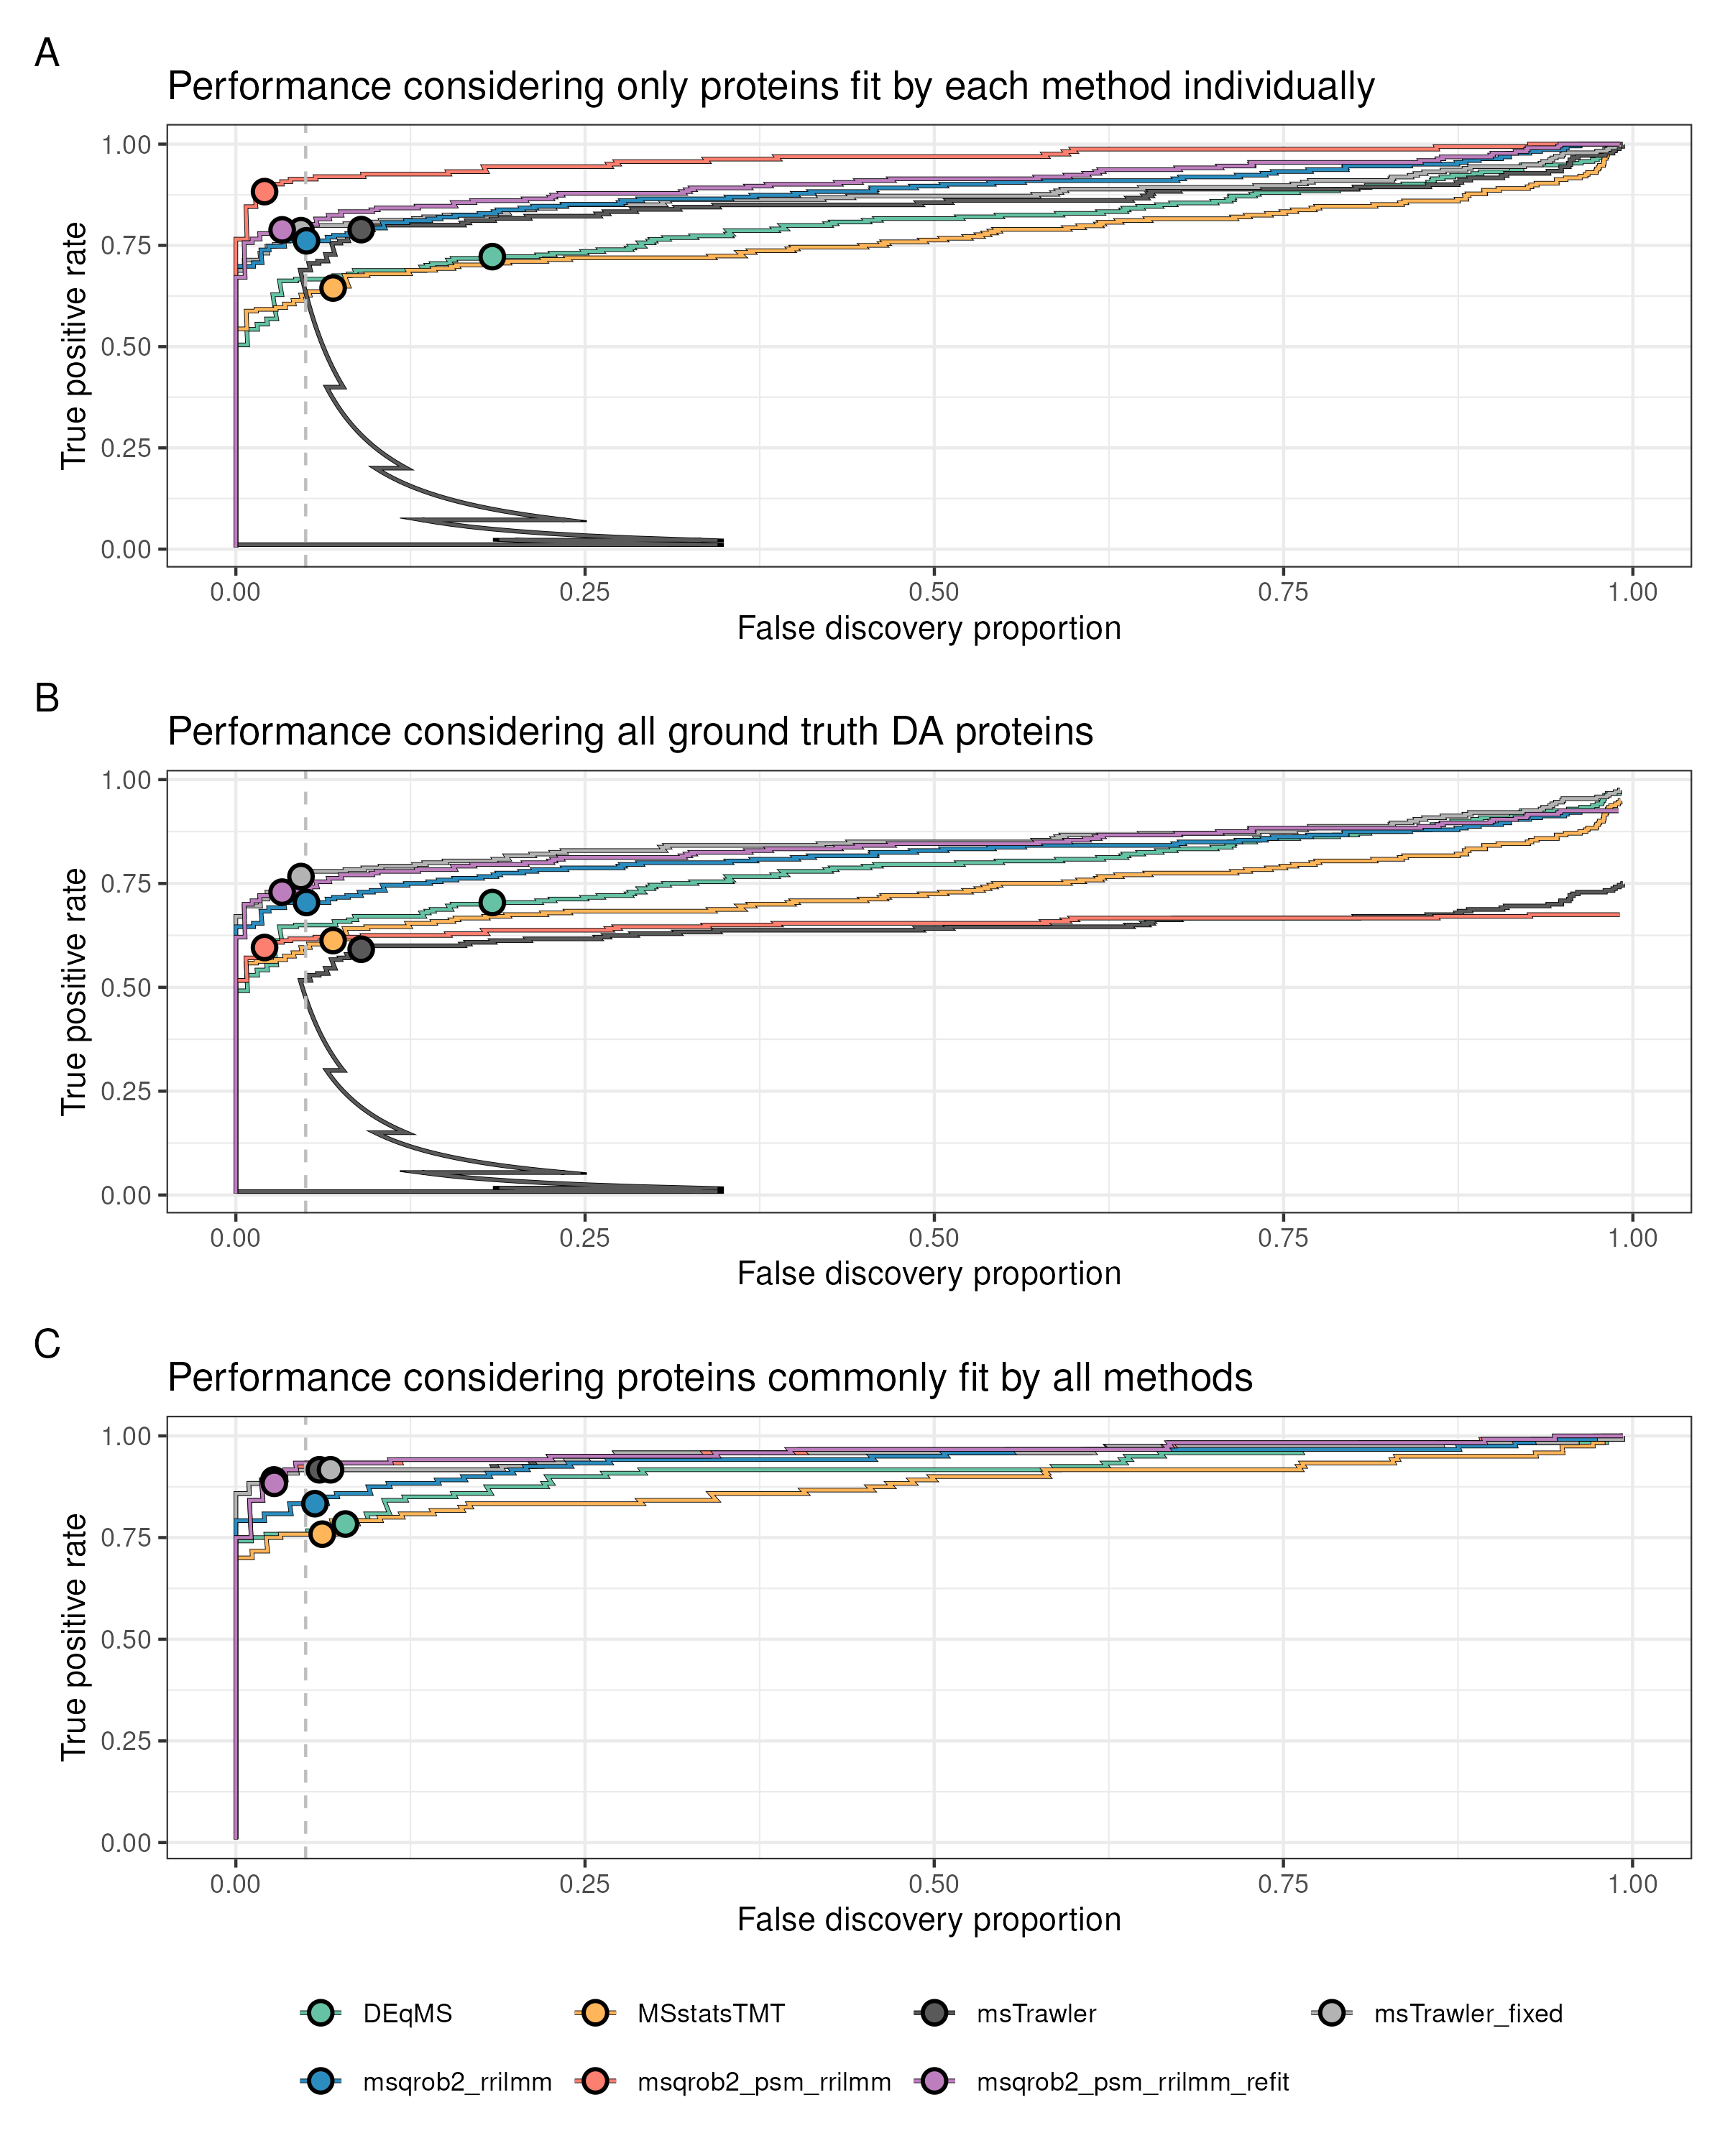
\includegraphics[width=0.9\textwidth,height=\textheight]{../figs/figureS1.png}

}

\caption{\label{fig-WorkflowComparisonsFull}True positive rate (TPR) -
false discovery proportion (FDP) plots for DEqMS, msqrob2TMT, msTrawler,
msTrawler~fixed with a refactored import function and MSstatsTMT
workflows based on all pairwise spike-in comparisons. Full Caption on
the next page.}

\end{figure}%

\textbf{Supplementary Figure }\ref{fig-WorkflowComparisonsFull}: True
positive rate (TPR) - false discovery proportion (FDP) plots for DEqMS,
msqrob2TMT, msTrawler, msTrawler\_fixed with a refactored import
function and MSstatsTMT workflows based on all pairwise spike-in
comparisons. In Panel A the performance is based on the results that are
returned by each workflow, in Panel B using all ground truth DA proteins
as the maximum number of true positives that can be reported for each
comparison (40 spike-in UPS proteins per comparison), and in panel C by
only considering the common proteins that were assessed by every
workflow. Dots indicate the TPR and FDP obtained at the 5\% FDR
threshold.

\begin{figure}[H]

\centering{

\includegraphics[width=1\textwidth,height=\textheight]{../figs/figureS2.png}

}

\caption{\label{fig-WorkflowComparisonsSeparateA}True positive rate
(TPR) - false discovery proportion (FDP) plots for DEqMS, MSstatsTMT,
msTrawler, msTrawler~fixed with a refactored import function and
msqrob2TMT workflows. The performance is based on the results that are
returned by each workflow. Dots indicate the TPR and FDP obtained at the
5\% FDR threshold.}

\end{figure}%

\begin{figure}[H]

\centering{

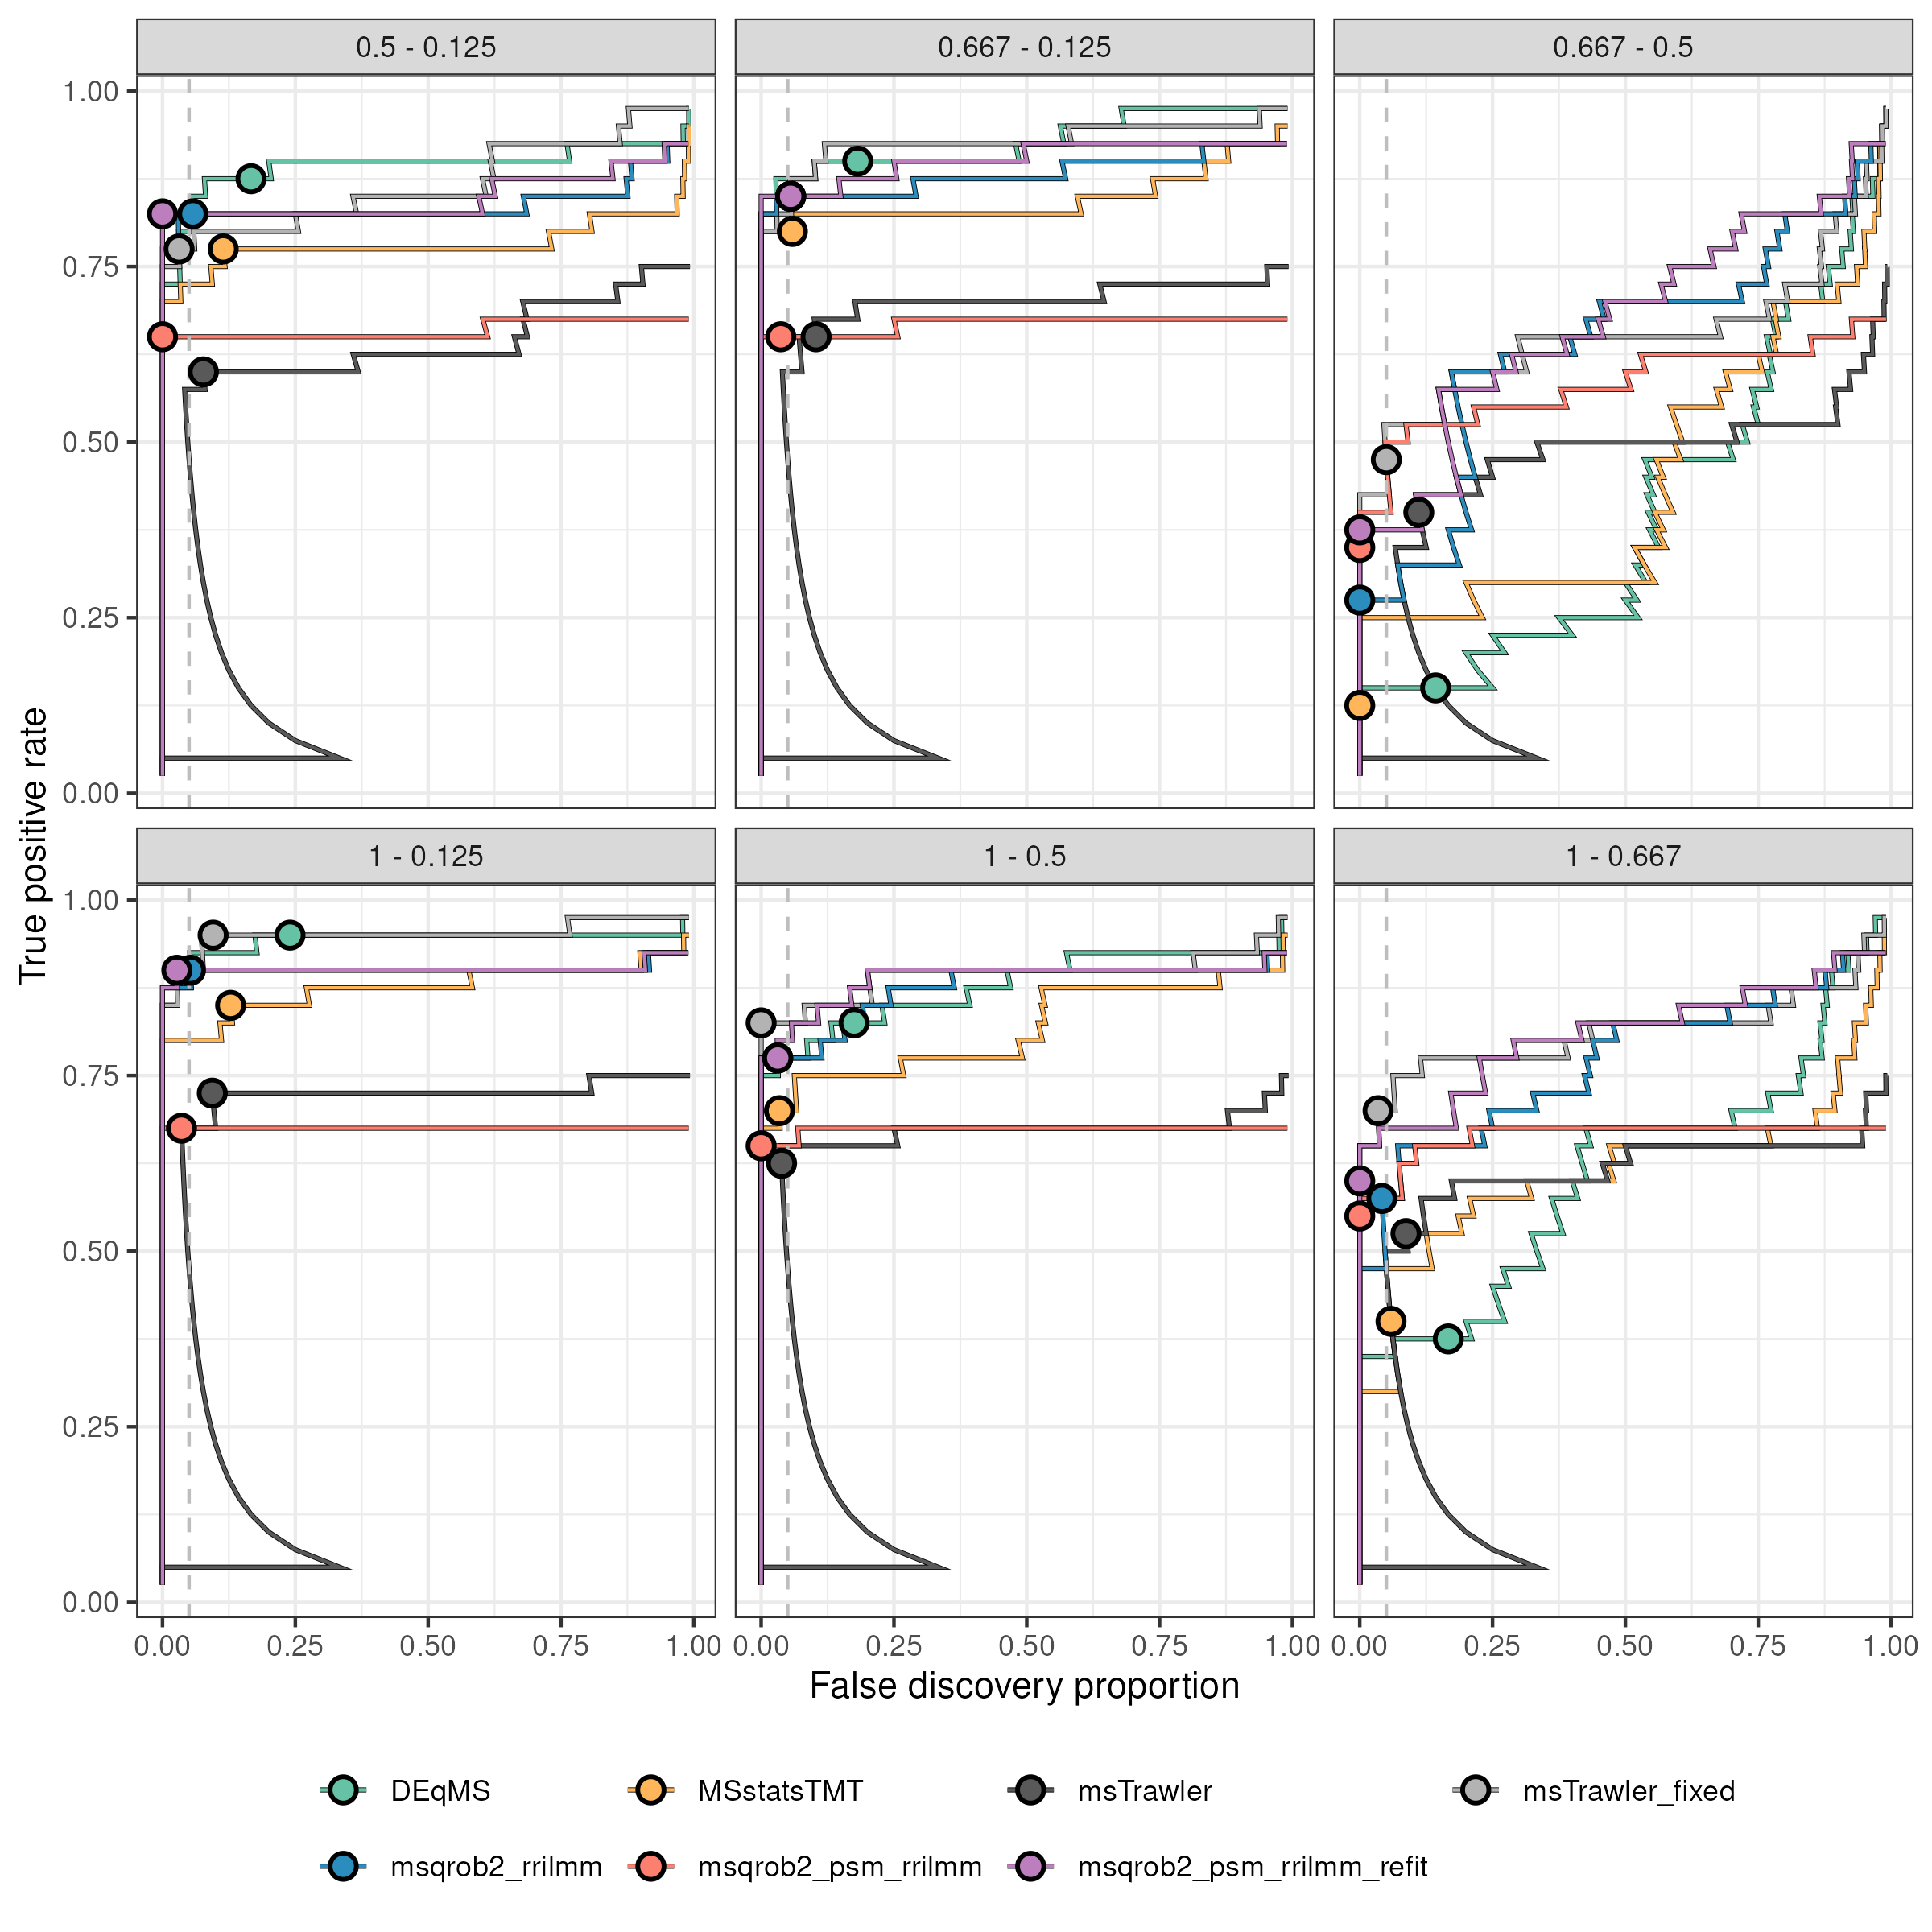
\includegraphics[width=1\textwidth,height=\textheight]{../figs/figureS3.png}

}

\caption{\label{fig-WorkflowComparisonsSeparateB}True positive rate
(TPR) - false discovery proportion (FDP) plots for DEqMS, MSstatsTMT,
msTrawler, msTrawler~fixed with a refactored import function and
msqrob2TMT workflows. The TPR is based on all ground truth DA proteins
as the maximum number of true positives that can be reported for each
comparison (40 spike-in UPS proteins). Dots indicate the TPR and FDP
obtained at the 5\% FDR threshold.}

\end{figure}%

\begin{figure}[H]

\centering{

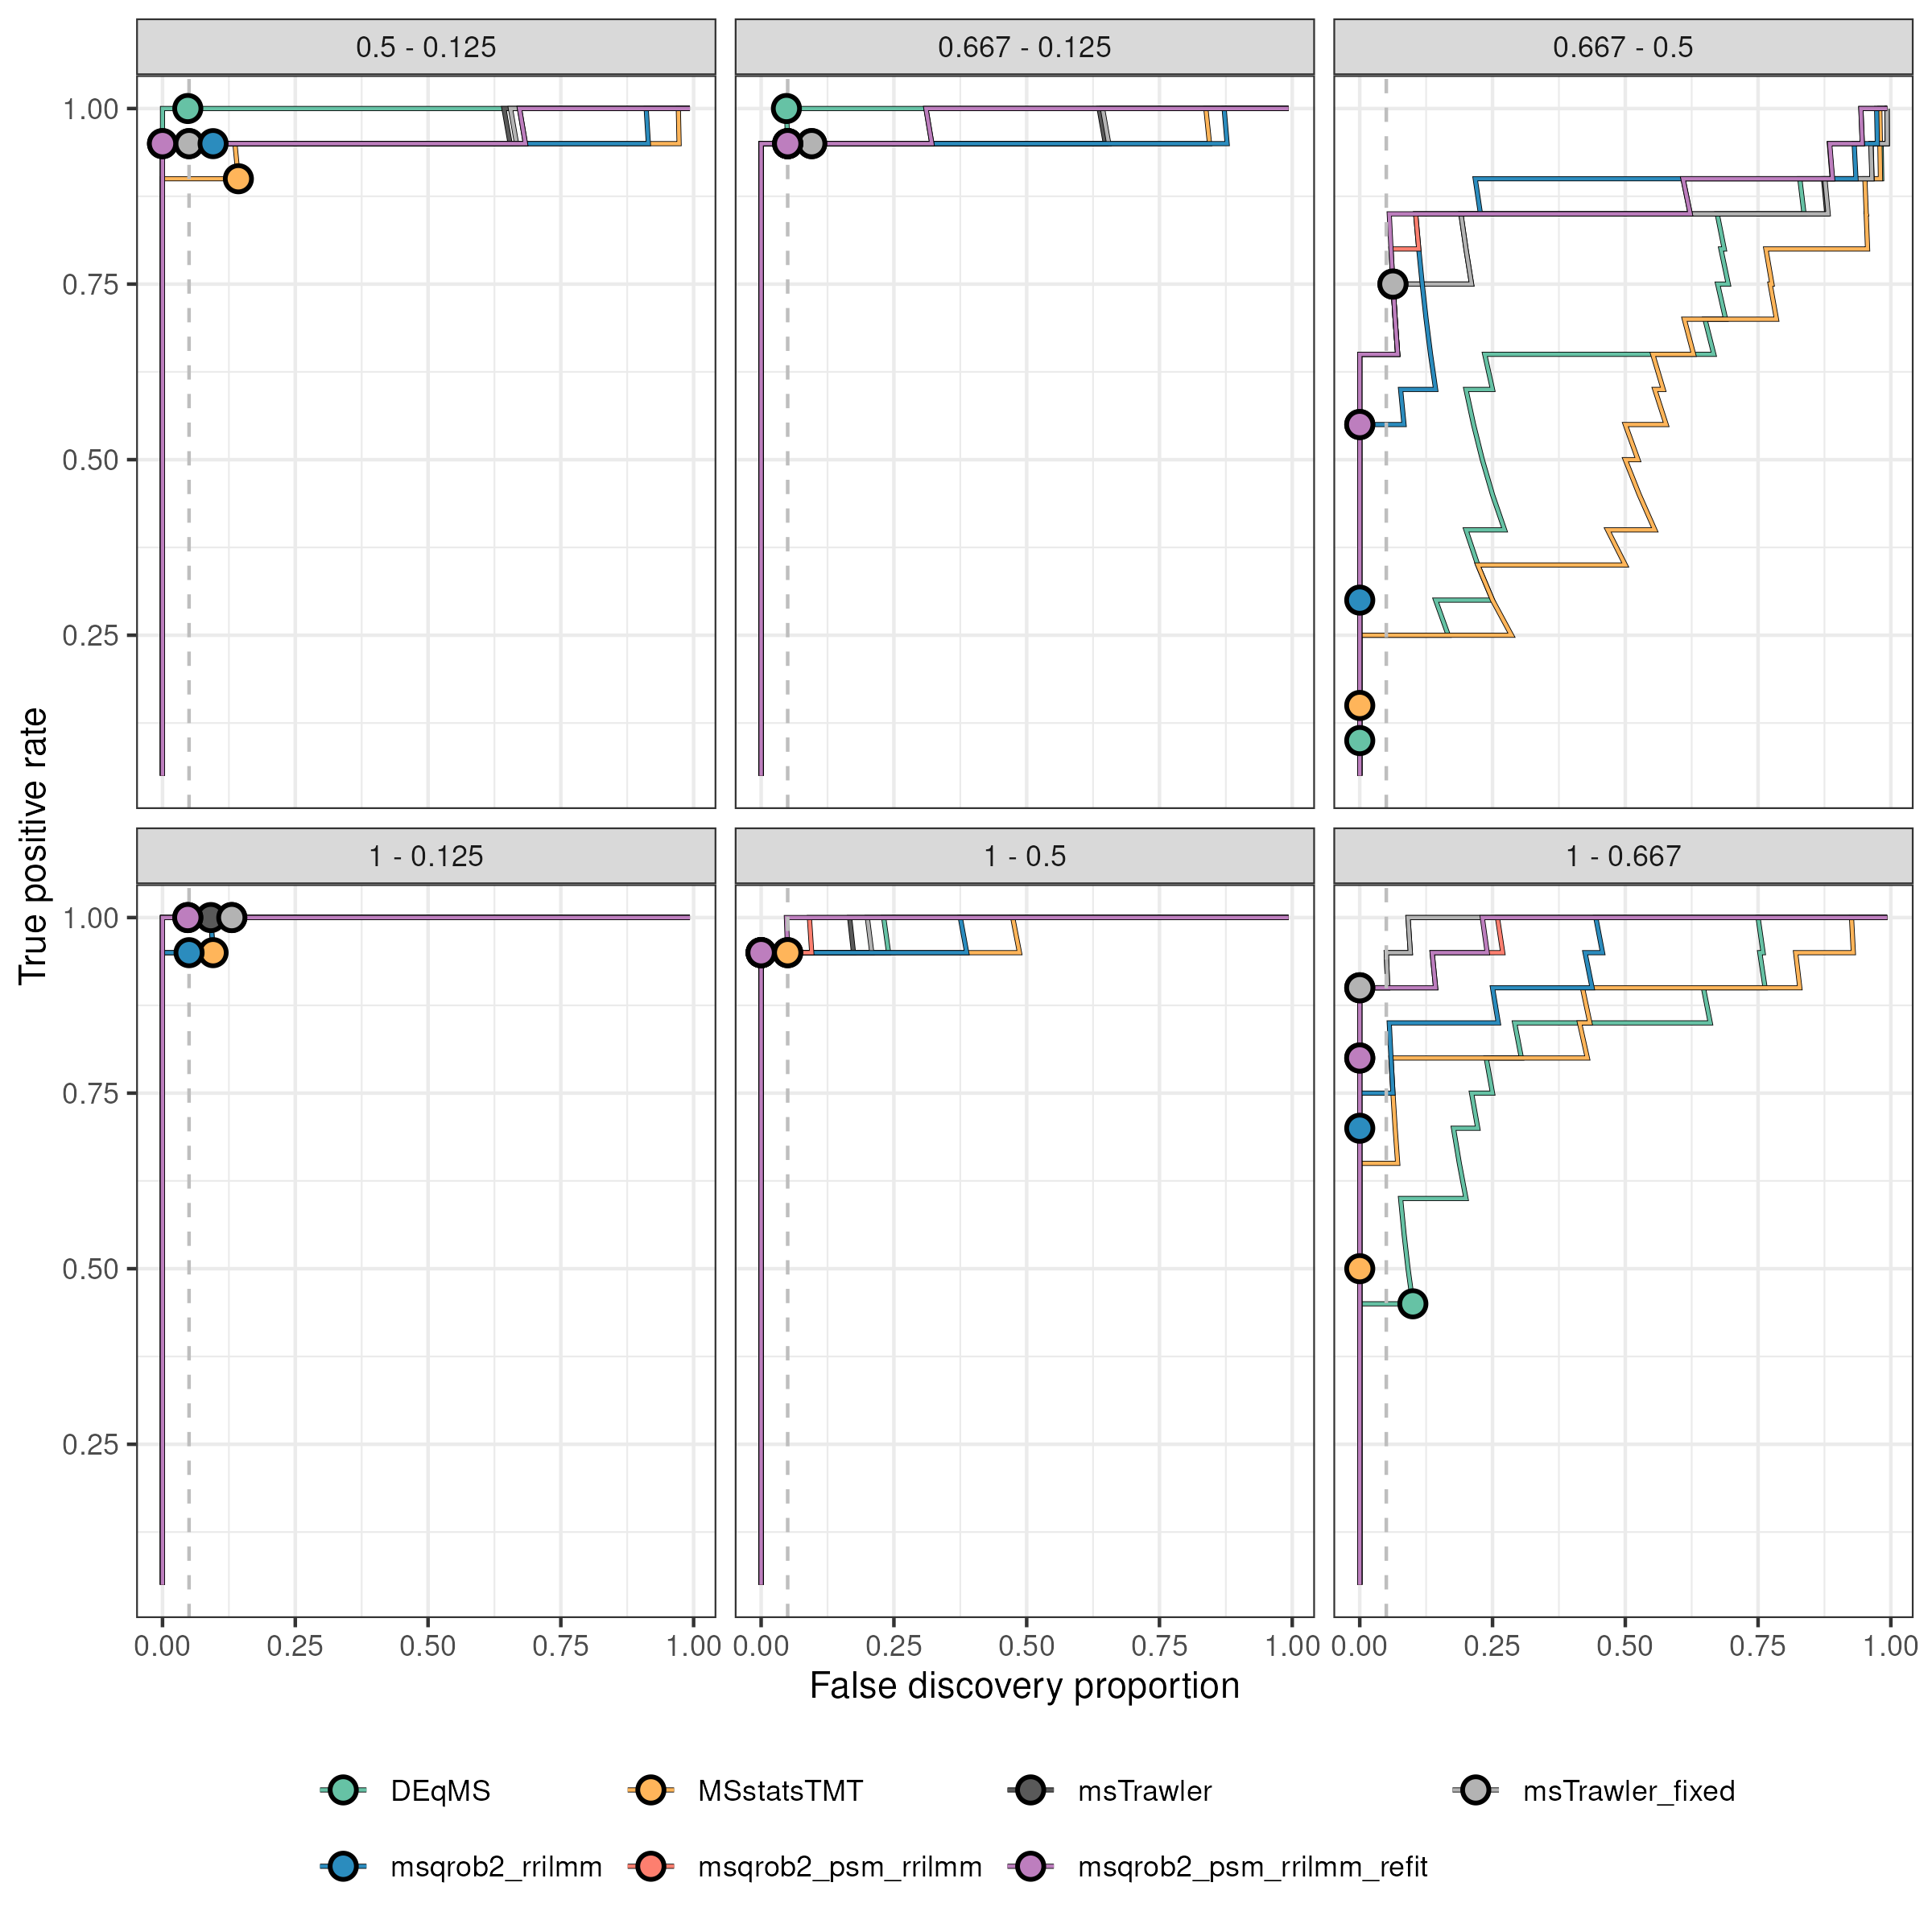
\includegraphics[width=1\textwidth,height=\textheight]{../figs/figureS4.png}

}

\caption{\label{fig-WorkflowComparisonsSeparateC}True positive rate
(TPR) - false discovery proportion (FDP) plots for DEqMS, MSstatsTMT,
msTrawler, msTrawler~fixed with a refactored import function and
msqrob2TMT workflows. The performance is based on the common proteins
that were assessed by every workflow. Dots indicate the TPR and FDP
obtained at the 5\% FDR threshold.}

\end{figure}%

\begin{figure}[H]

\centering{

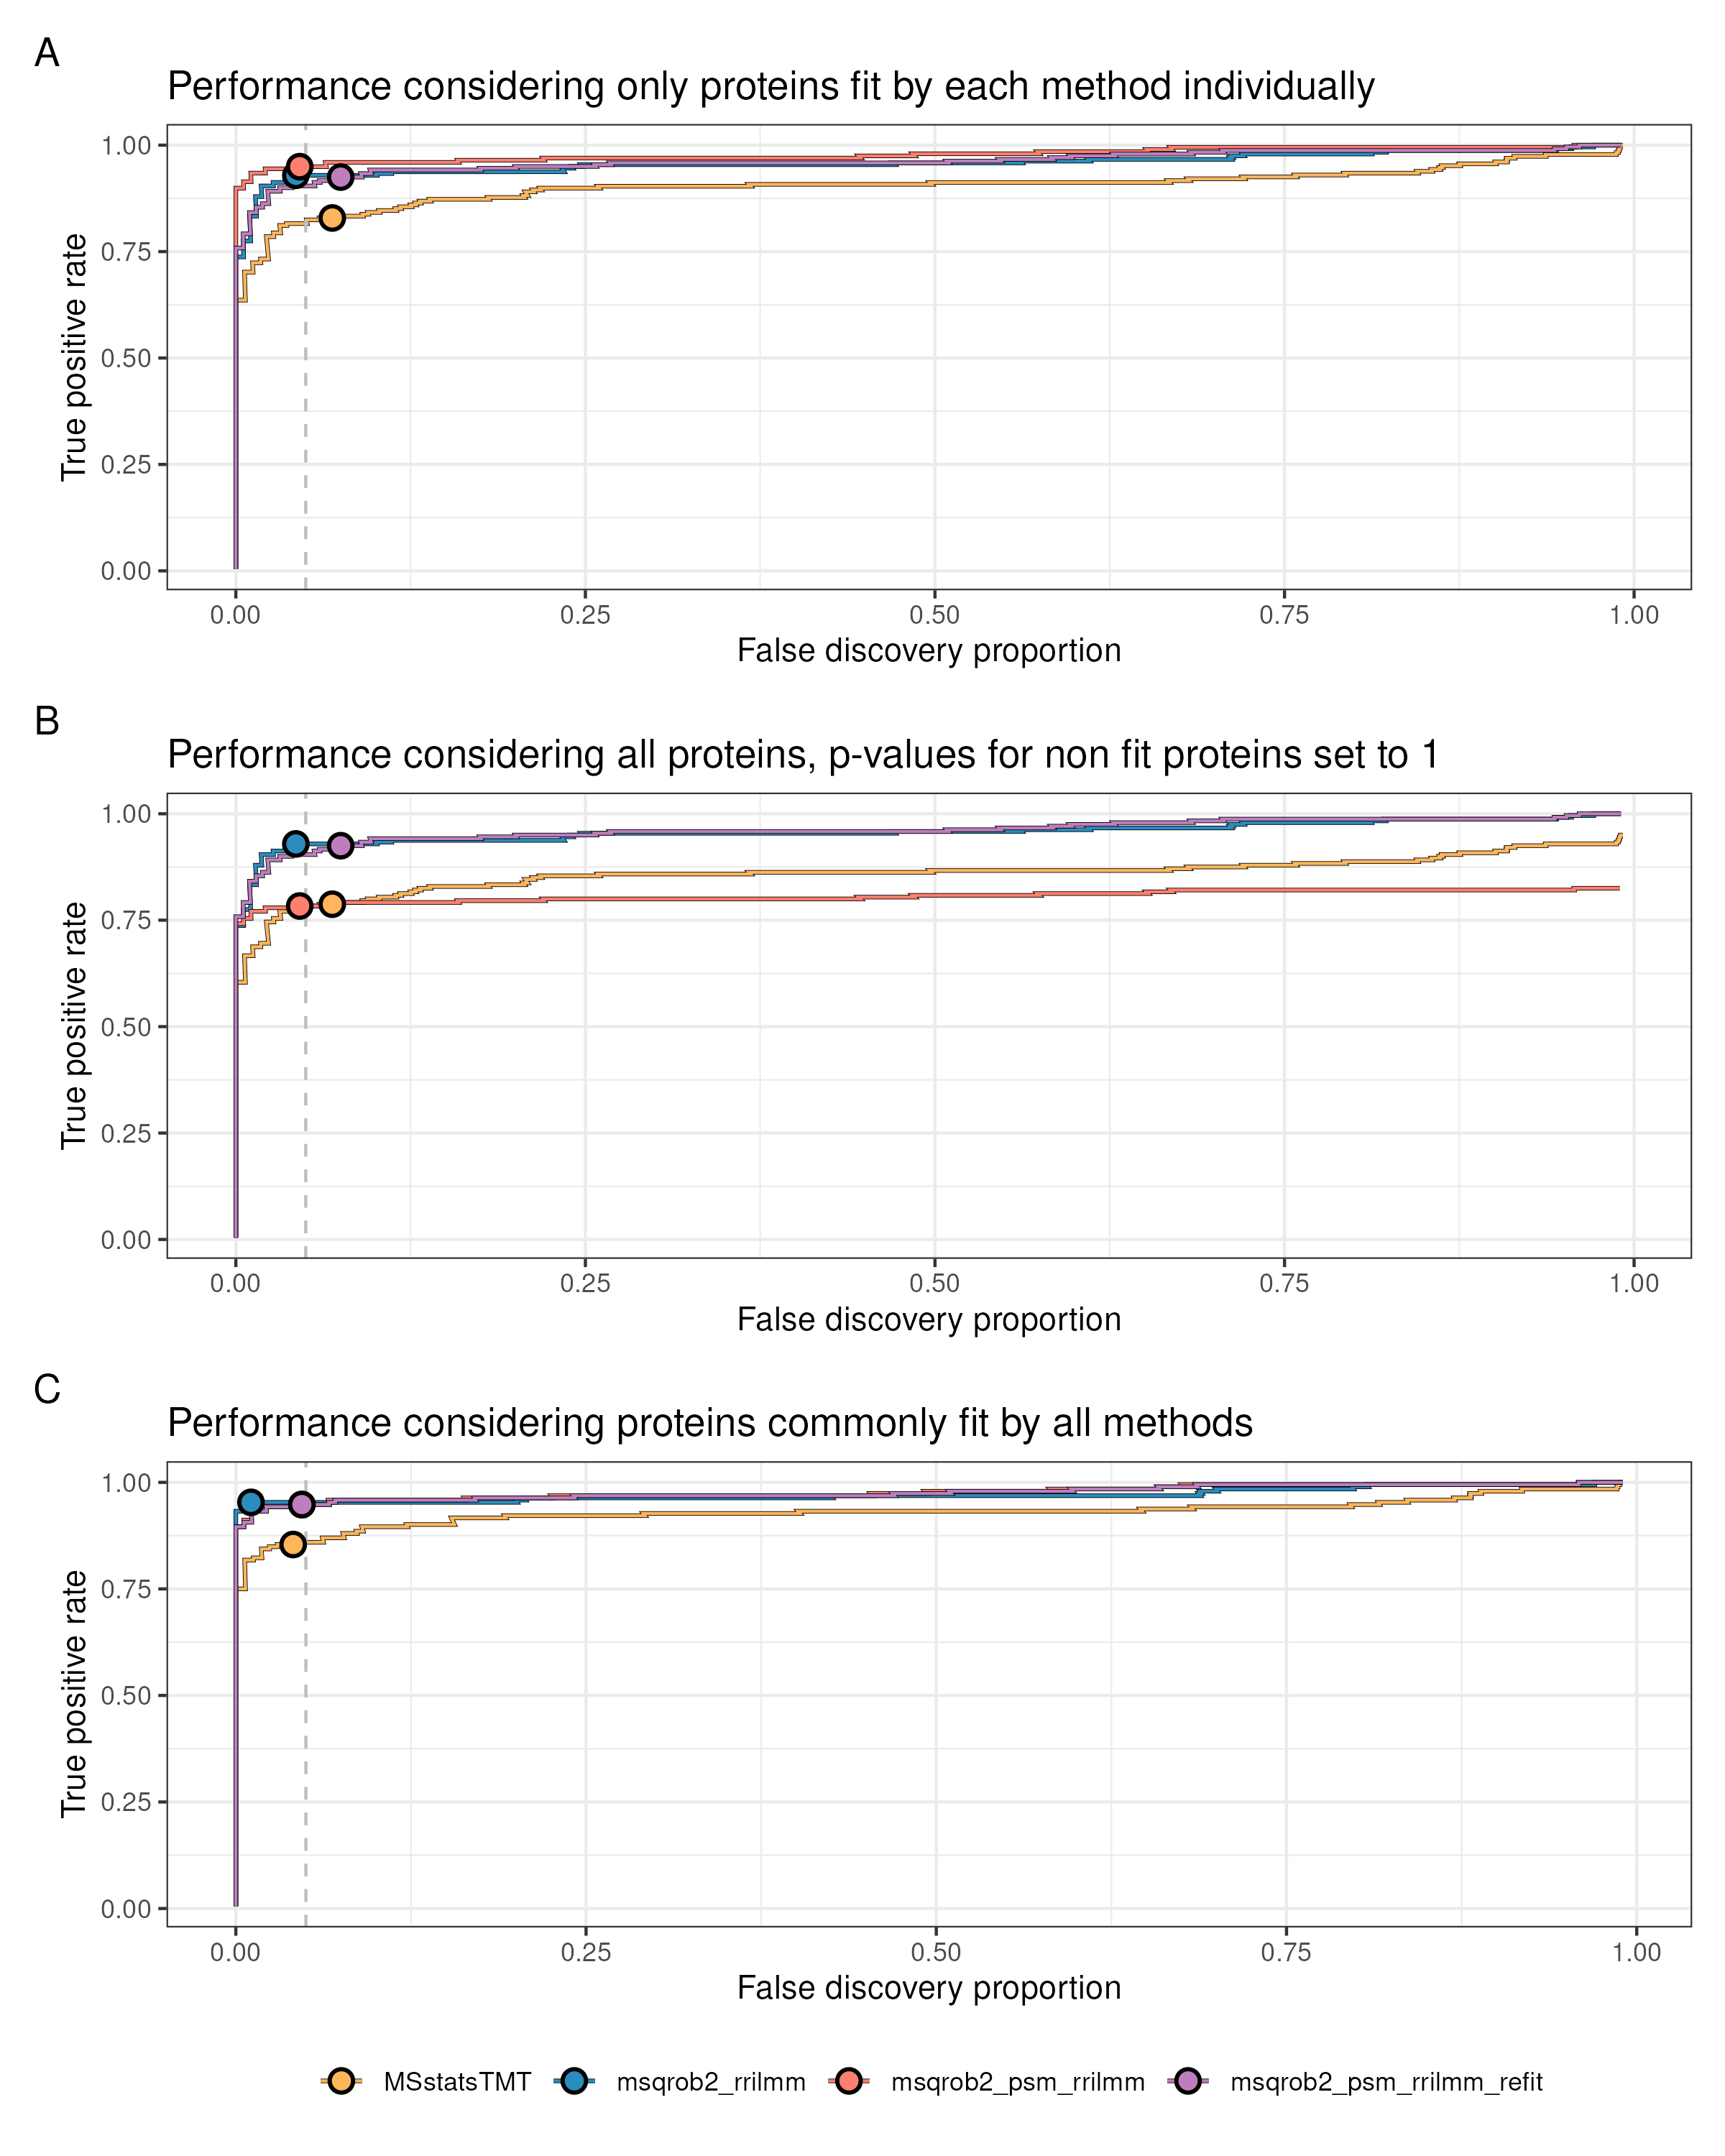
\includegraphics[width=0.9\textwidth,height=\textheight]{../figs/figureS5.png}

}

\caption{\label{fig-WorkflowComparisonsTechreps}True positive rate (TPR)
- false discovery proportion (FDP) plots for MSstatsTMT and msqrob2TMT
workflows using all technical repeats. The performance is based on all
pairwise spike-in comparisons and only considering the results that are
returned by each workflow (Panel A), all ground truth DA proteins as the
maximum number of true positives that can be reported for each
comparison (panel B), and the common proteins that were assessed by
every method (panel C). Dots indicate the TPR and FDP obtained at the
5\% FDR threshold.}

\end{figure}%

\begin{figure}[H]

\centering{

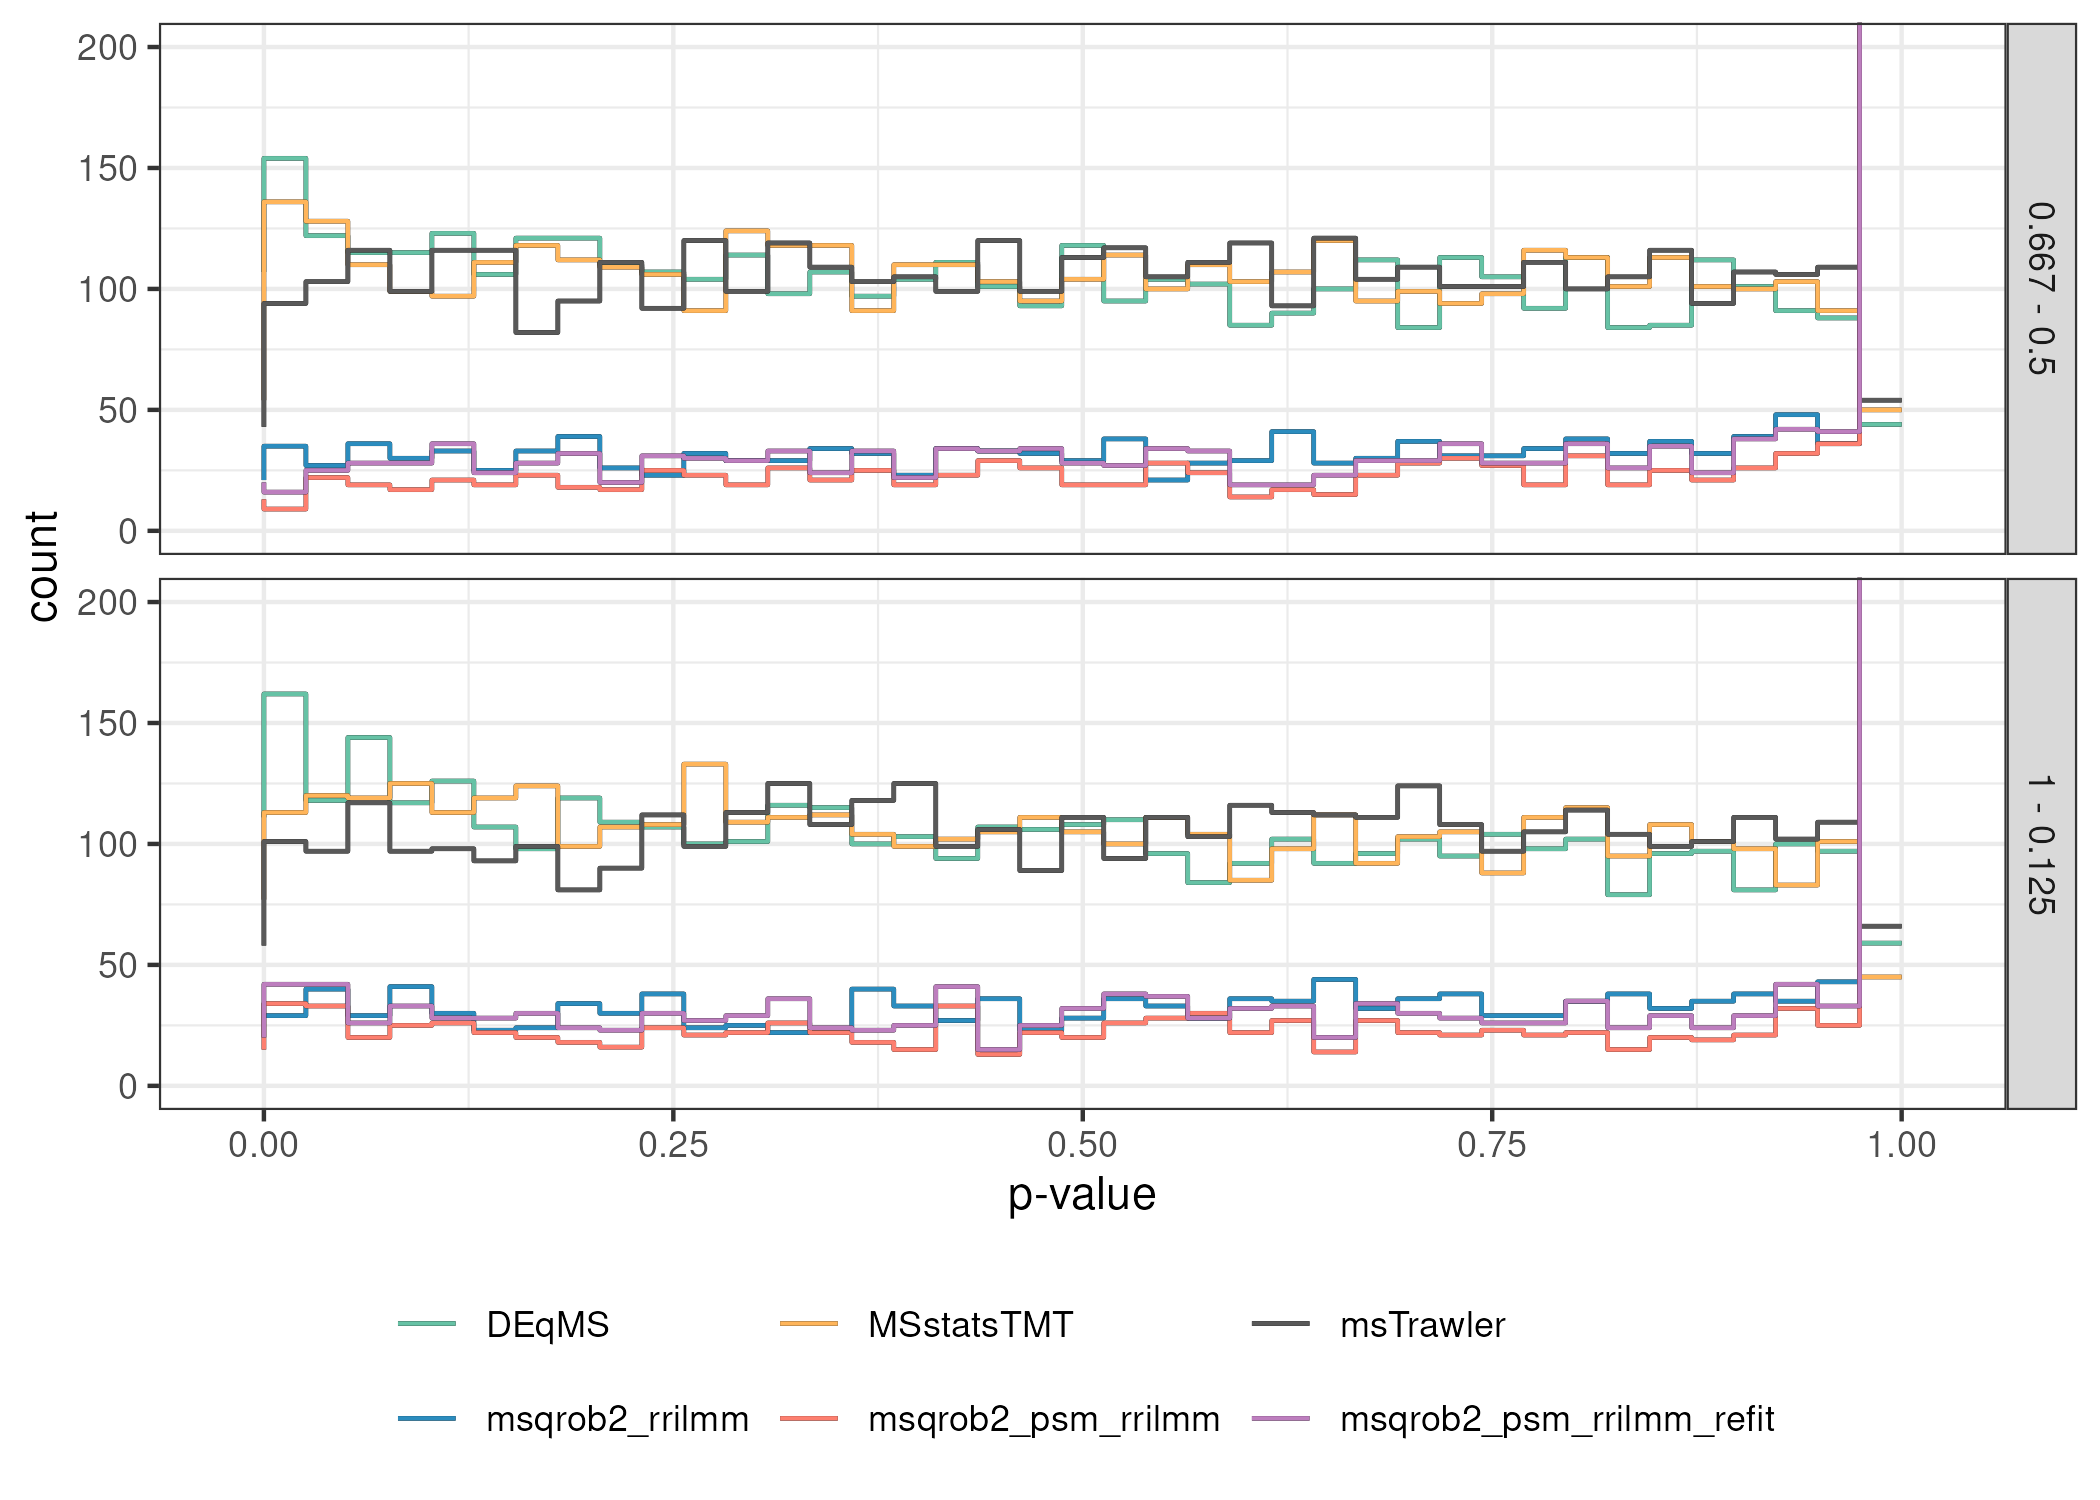
\includegraphics[width=1\textwidth,height=\textheight]{../figs/figureS6.png}

}

\caption{\label{fig-spikein1_pvalue_dist_nondiff}Histograms of the
p-values from non-spike-in proteins for the DEqMS, msqrob2TMT,
MSstatsTMT and msTrawler workflows for two distinct pairwise comparisons
between spike-in dilutions.}

\end{figure}%

\begin{figure}[H]

\centering{

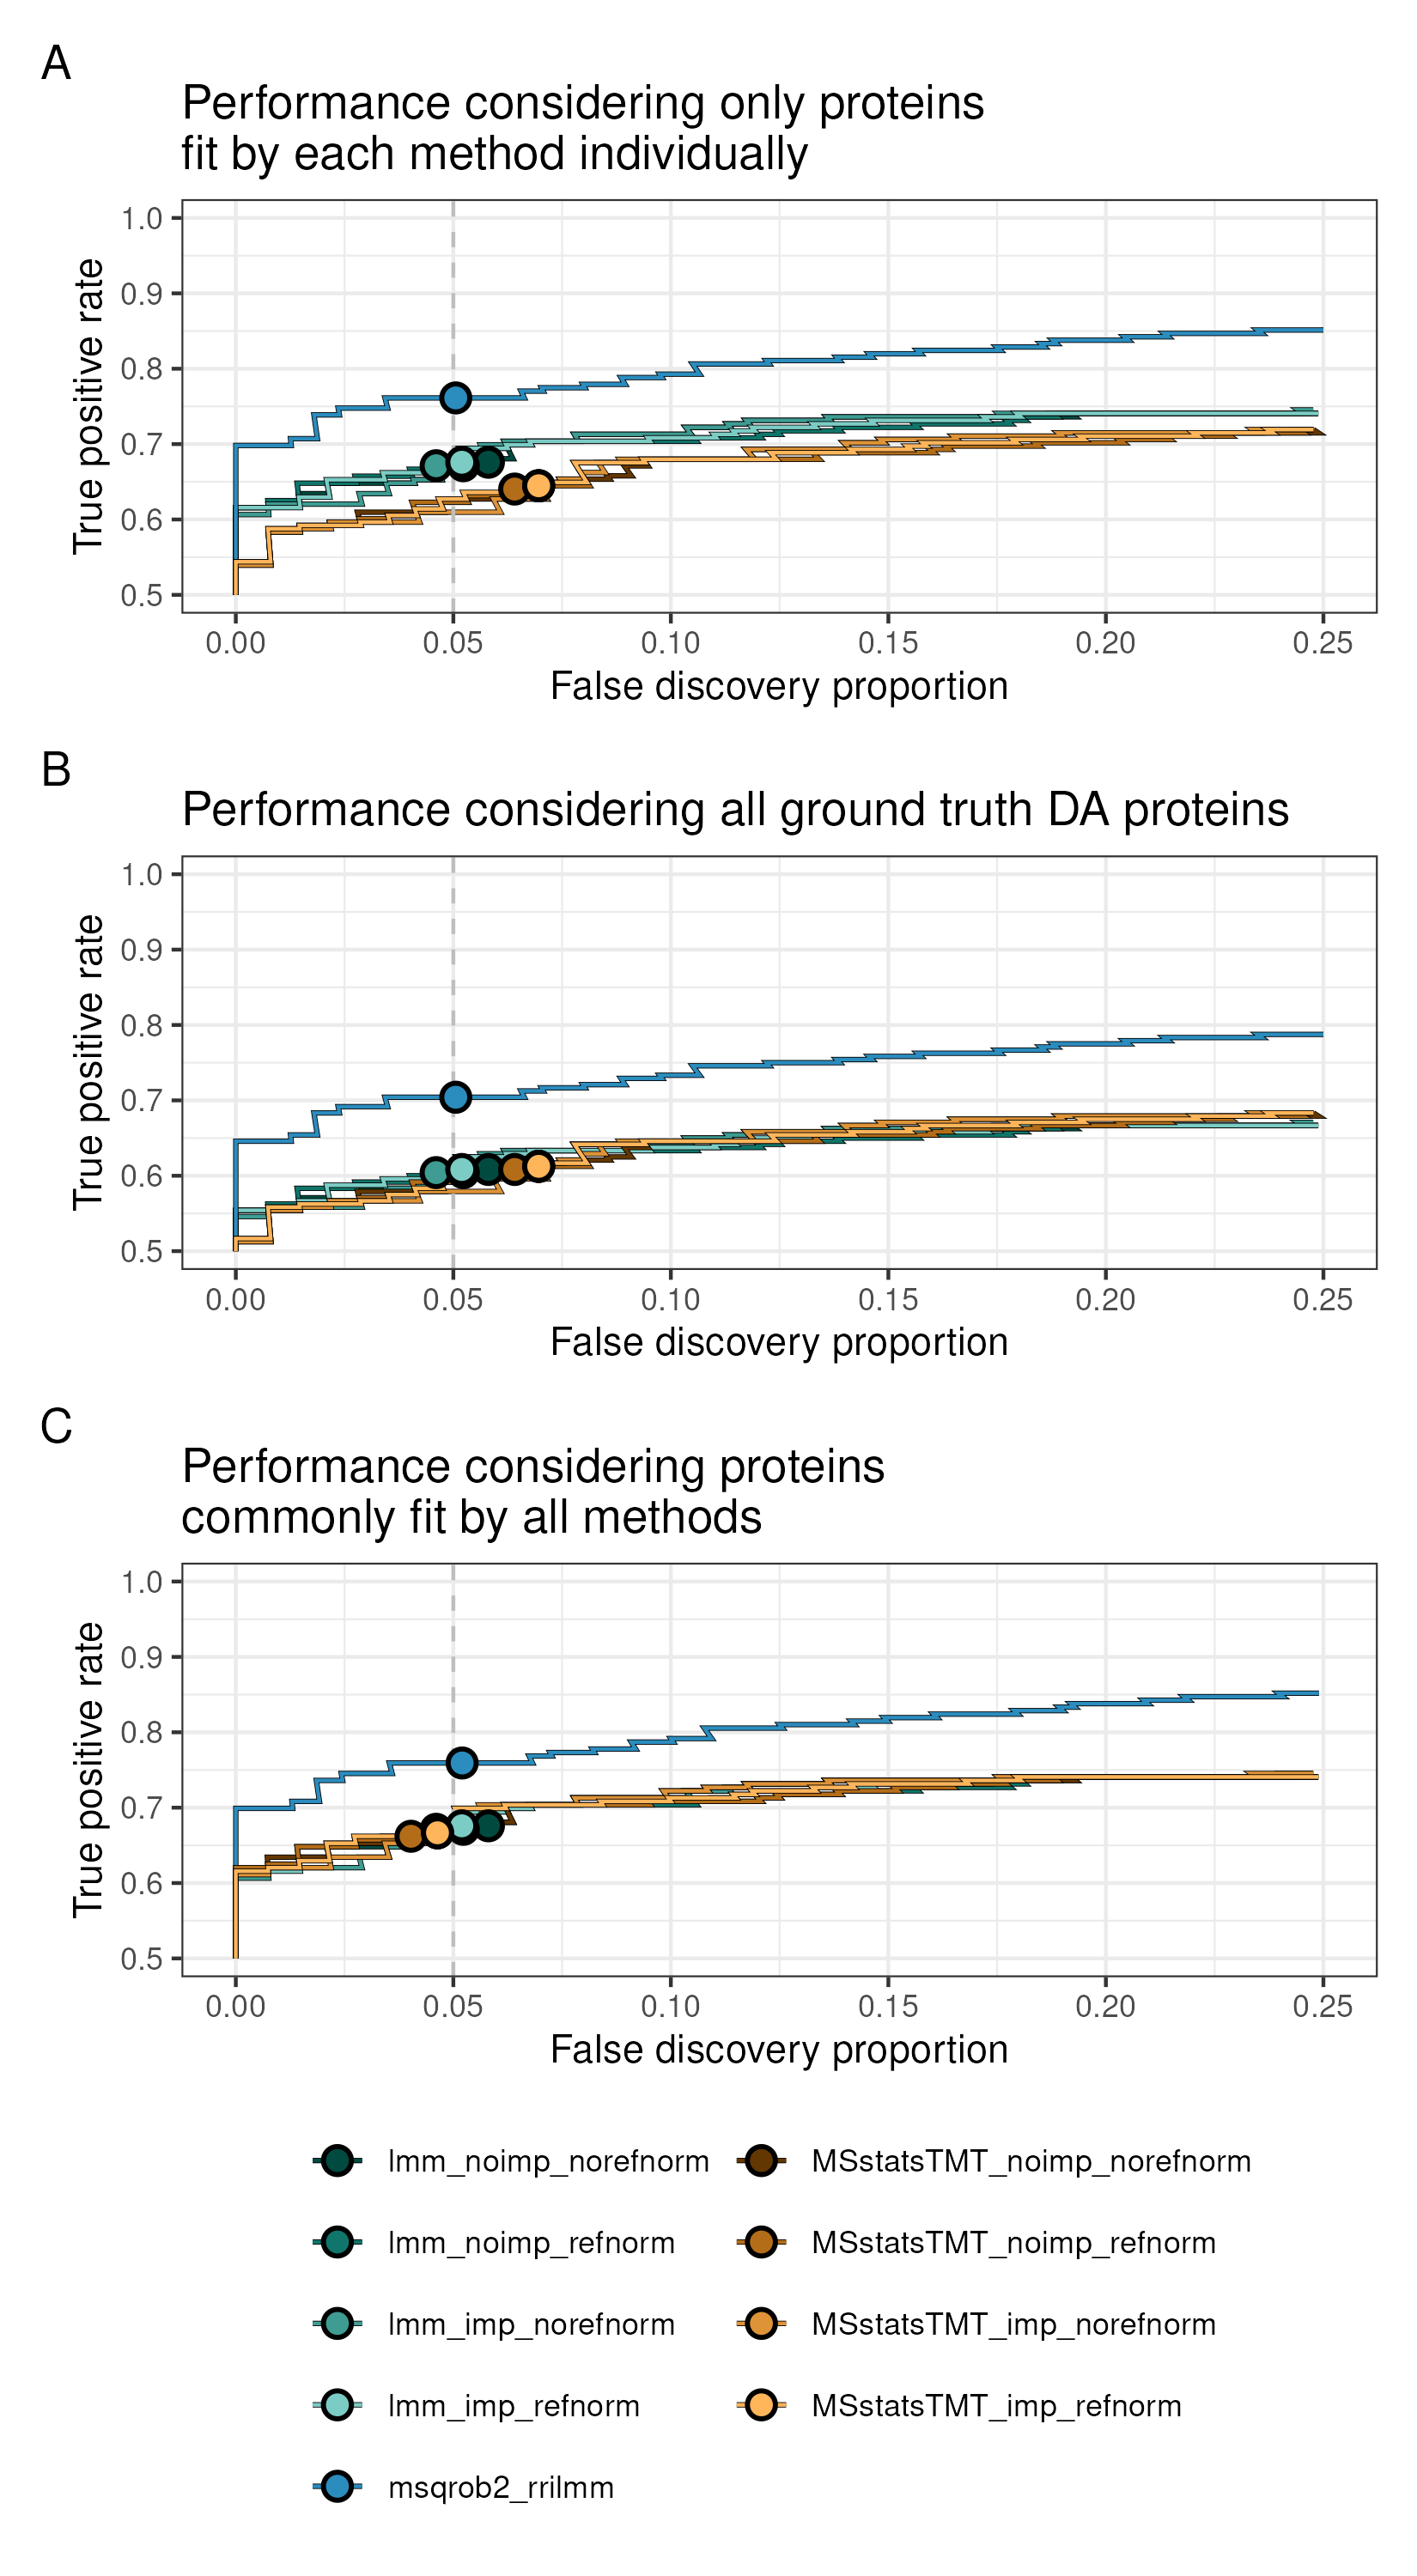
\includegraphics[width=1\textwidth,height=\textheight]{../figs/figureS7.png}

}

\caption{\label{fig-WorkflowComparisonsPreprocessing}Caption on the next
page.}

\end{figure}%

\textbf{Supplementary Figure }
\ref{fig-WorkflowComparisonsPreprocessing}: True positive rate (TPR) -
false discovery proportion (FDP) illustrating the effect of the
MSstatsTMT preprocessing on the performance for the msqrob2TMT
protein-level models. MSstatsTMT preprocessing was conducted both with
and without imputation, employing its accelerated failure time model,
and, with and without reference normalisation using bridge channels.
These configurations are denoted with the suffixes -noimp (no
imputation), -imp (with imputation), -norefnorm (no reference
normalisation) and -refnorm (with reference normalisation),
respectively. Differential abundance on the preprocessed, summarised and
normalised protein abundances was subsequently inferred with MSstatsTMT,
msqrob2TMT with a vanilla linear mixed model (lmm) or msqrob2TMT
employing a linear mixed model fitted via robust M-estimation and ridge
regression (rrilmm). The combined performance over all the spike-in
comparisons are shown. In Panel A the performance is based on the
results that are returned by each workflow, in Panel B on all ground
truth DA proteins per comparison (40 spike-in UPS proteins per
comparison) and in Panel C by only considering the common proteins that
were assessed by every workflow. Dots indicate the TPR and FDP obtained
at the 5\% FDR threshold.

\section*{Multibatch Benchmarking Experiment}

\begin{figure}[H]

\centering{

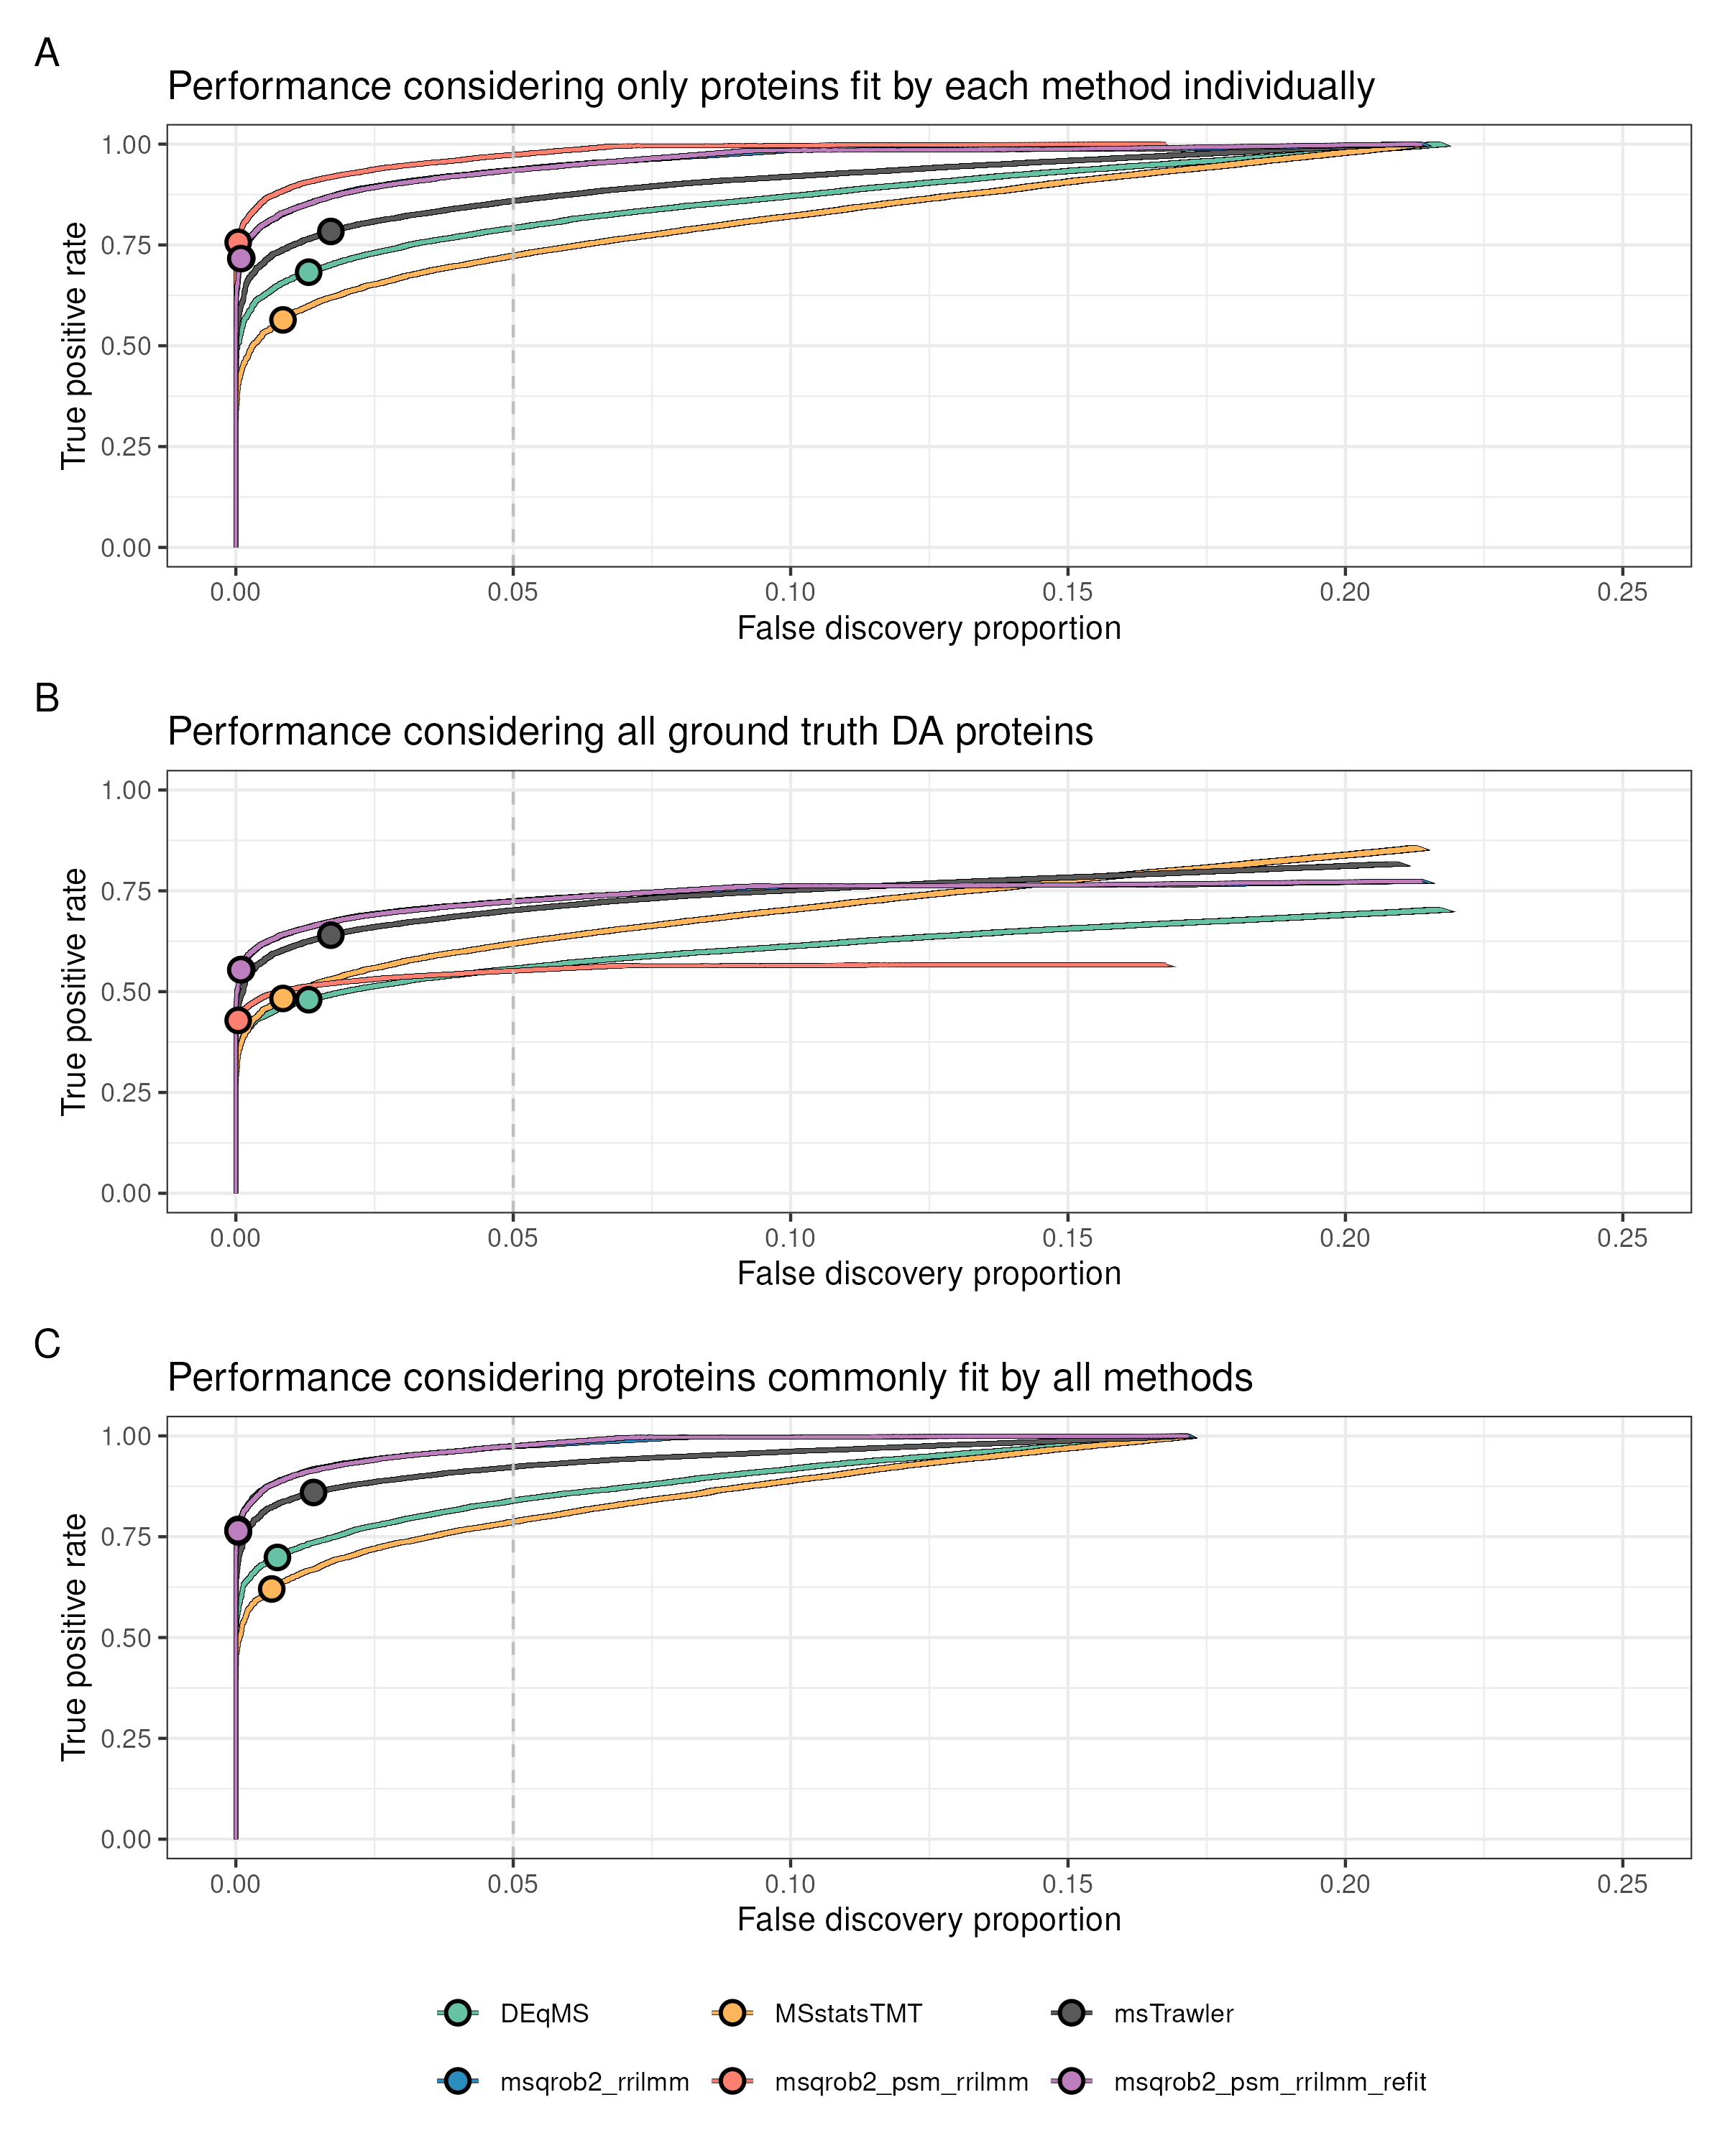
\includegraphics[width=1\textwidth,height=\textheight]{../figs/figureS8.png}

}

\caption{\label{fig-WorkflowComparisonsSpikein2ALL}Caption on the next
page.}

\end{figure}%

\textbf{Supplementary Figure } \ref{fig-WorkflowComparisonsSpikein2ALL}:
True positive rate (TPR) - false discovery proportion (FDP) plots for
DEqMS, MSstatsTMT, msTrawler and msqrob2TMT workflows. The combined
performance over all the comparisons are shown. In Panel A the
performance is based on the results that are returned by each workflow,
in Panel B on all ground truth DA proteins as the maximum number of true
positives that can be reported for each comparison, and in panel C by
only considering the common proteins that were assessed by every
workflow. Dots indicate the TPR and FDP obtained at the 5\% FDR
threshold.

\begin{figure}[H]

\centering{

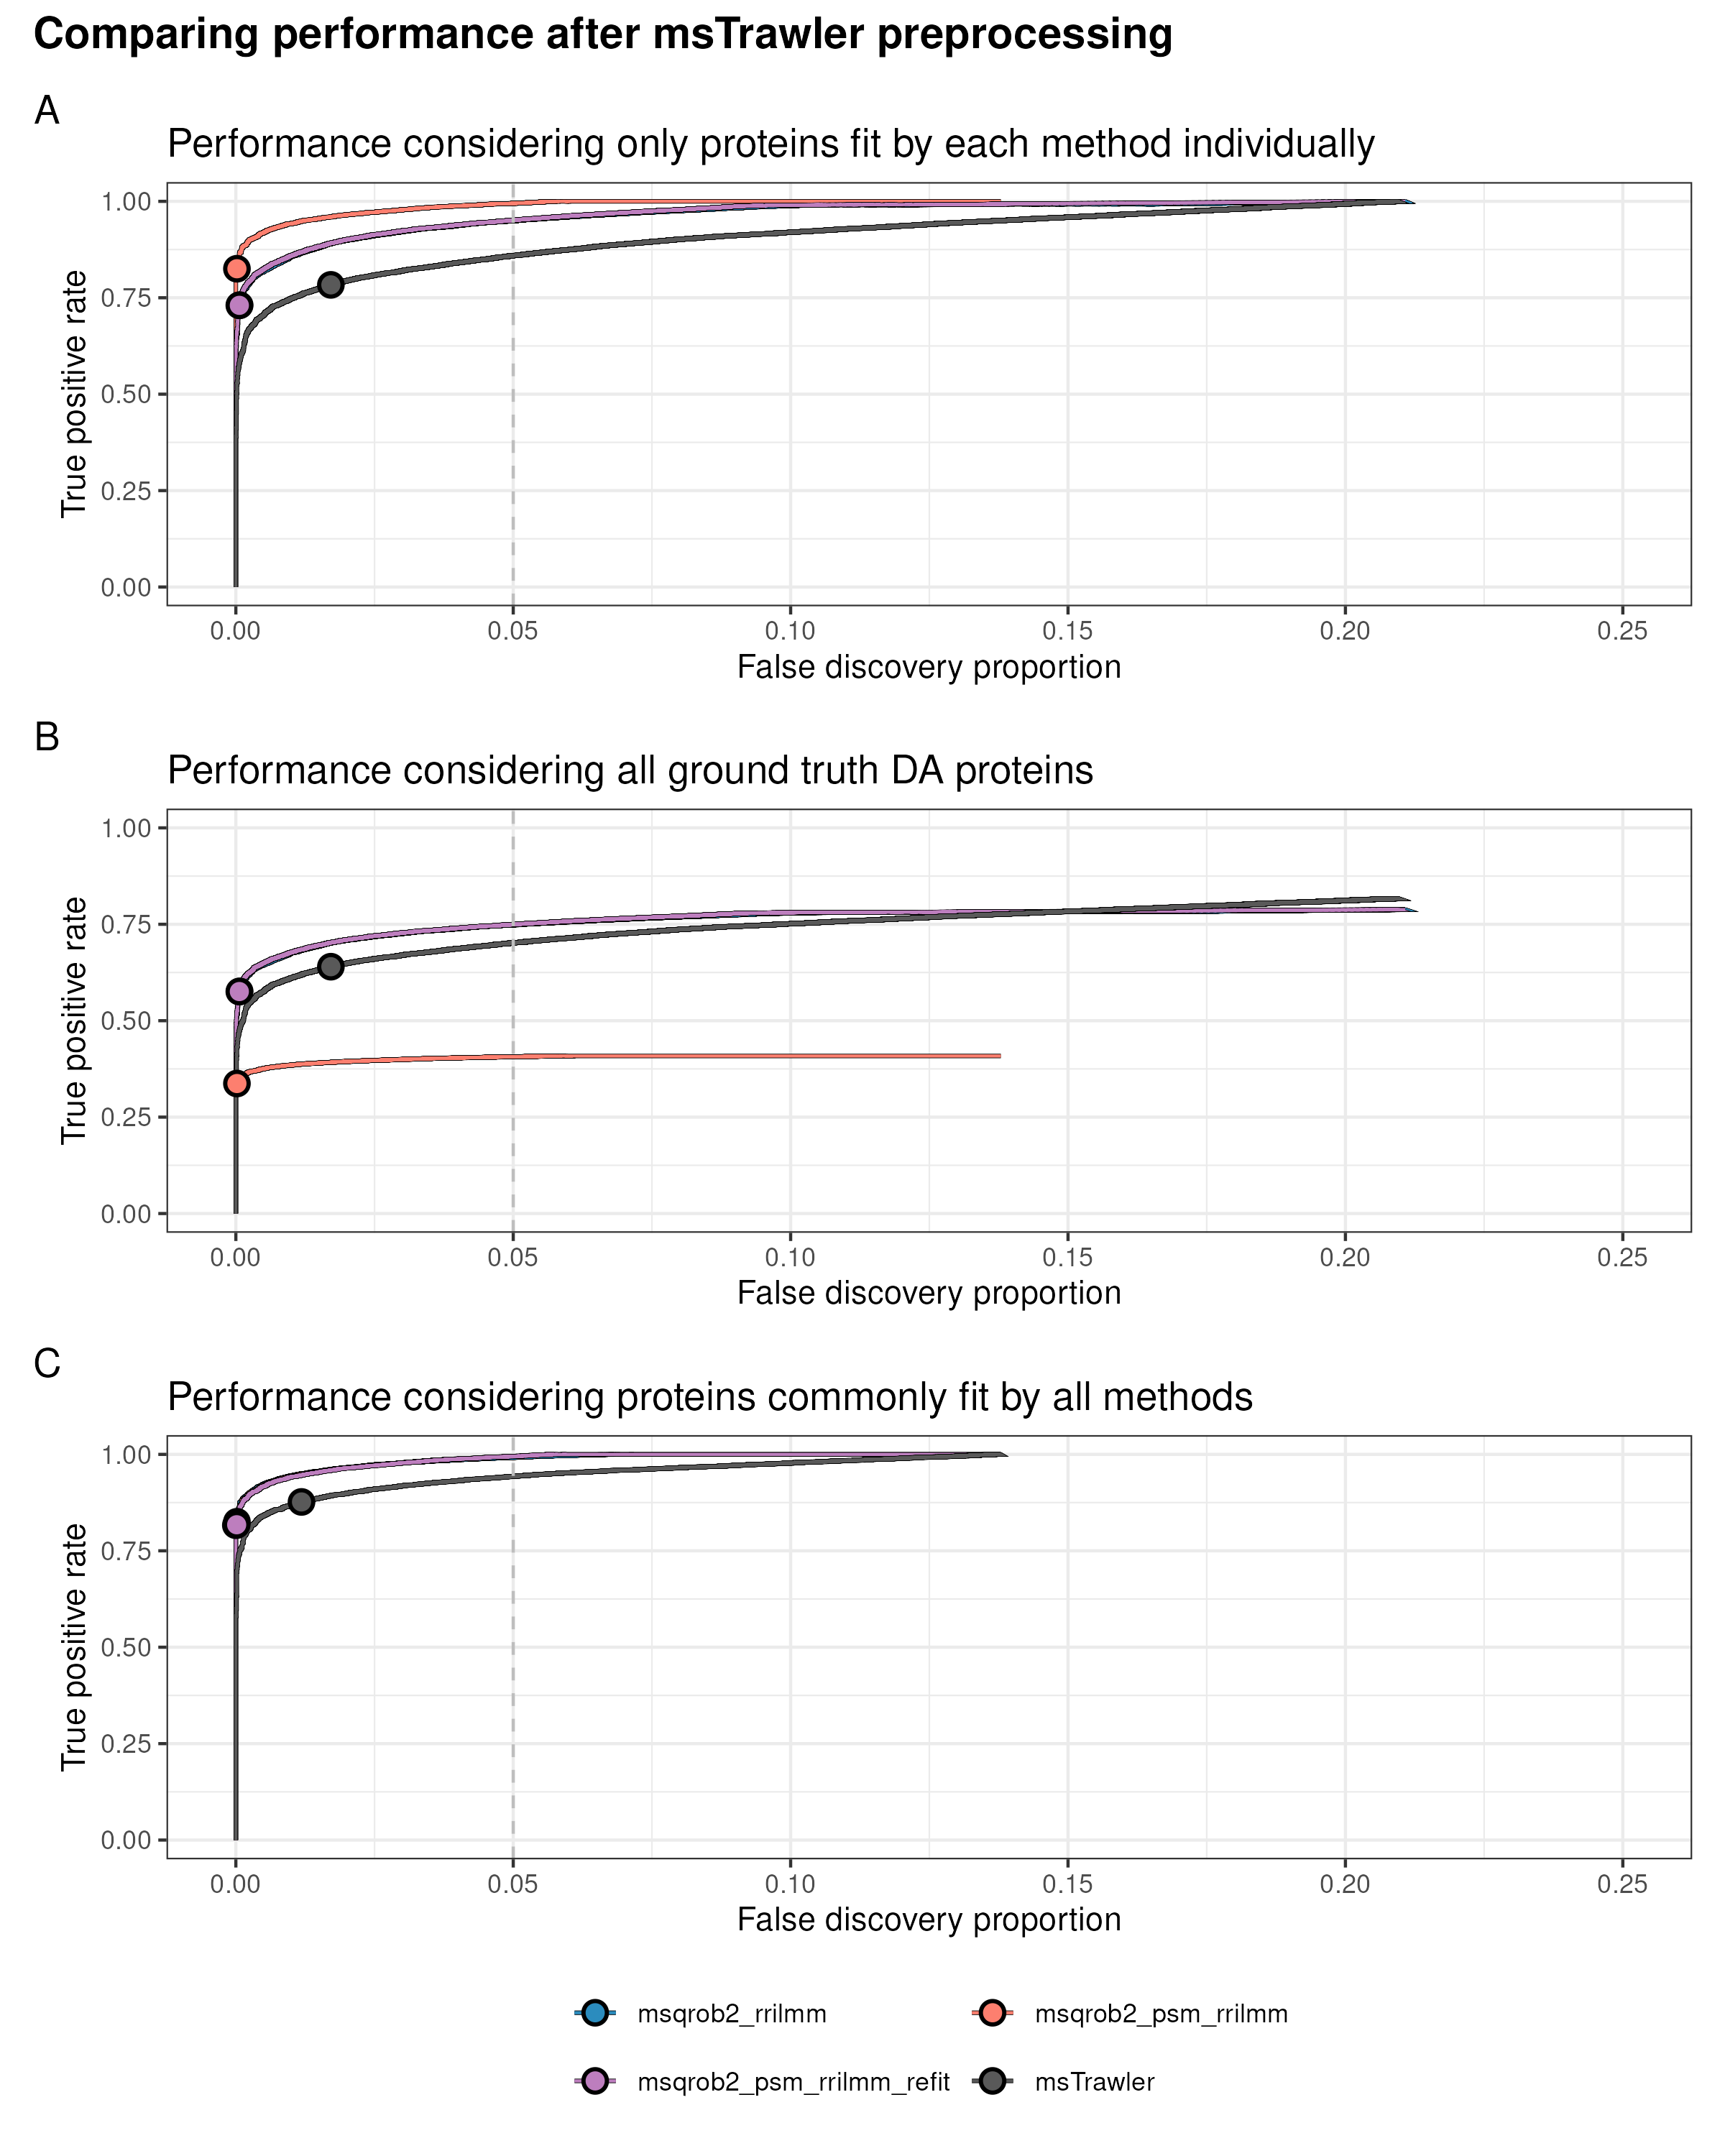
\includegraphics[width=0.9\textwidth,height=\textheight]{../figs/figureS9.png}

}

\caption{\label{fig-WorkflowComparisonsPreprocessingSpikein2}True
positive rate (TPR) - false discovery proportion (FDP) plots for DEqMS,
MSstatsTMT, msTrawler and msqrob2TMT workflows upon full msTrawler
preprocessing. The combined performance over all the comparisons are
shown. In Panel A the performance is based on the results that are
returned by each workflow, in Panel B on all ground truth DA proteins as
the maximum number of true positives that can be reported for each
comparison, and in panel C by only considering the common proteins that
were assessed by every workflow. Dots indicate the TPR and FDP obtained
at the 5\% FDR threshold.}

\end{figure}%

\begin{figure}[H]

\centering{

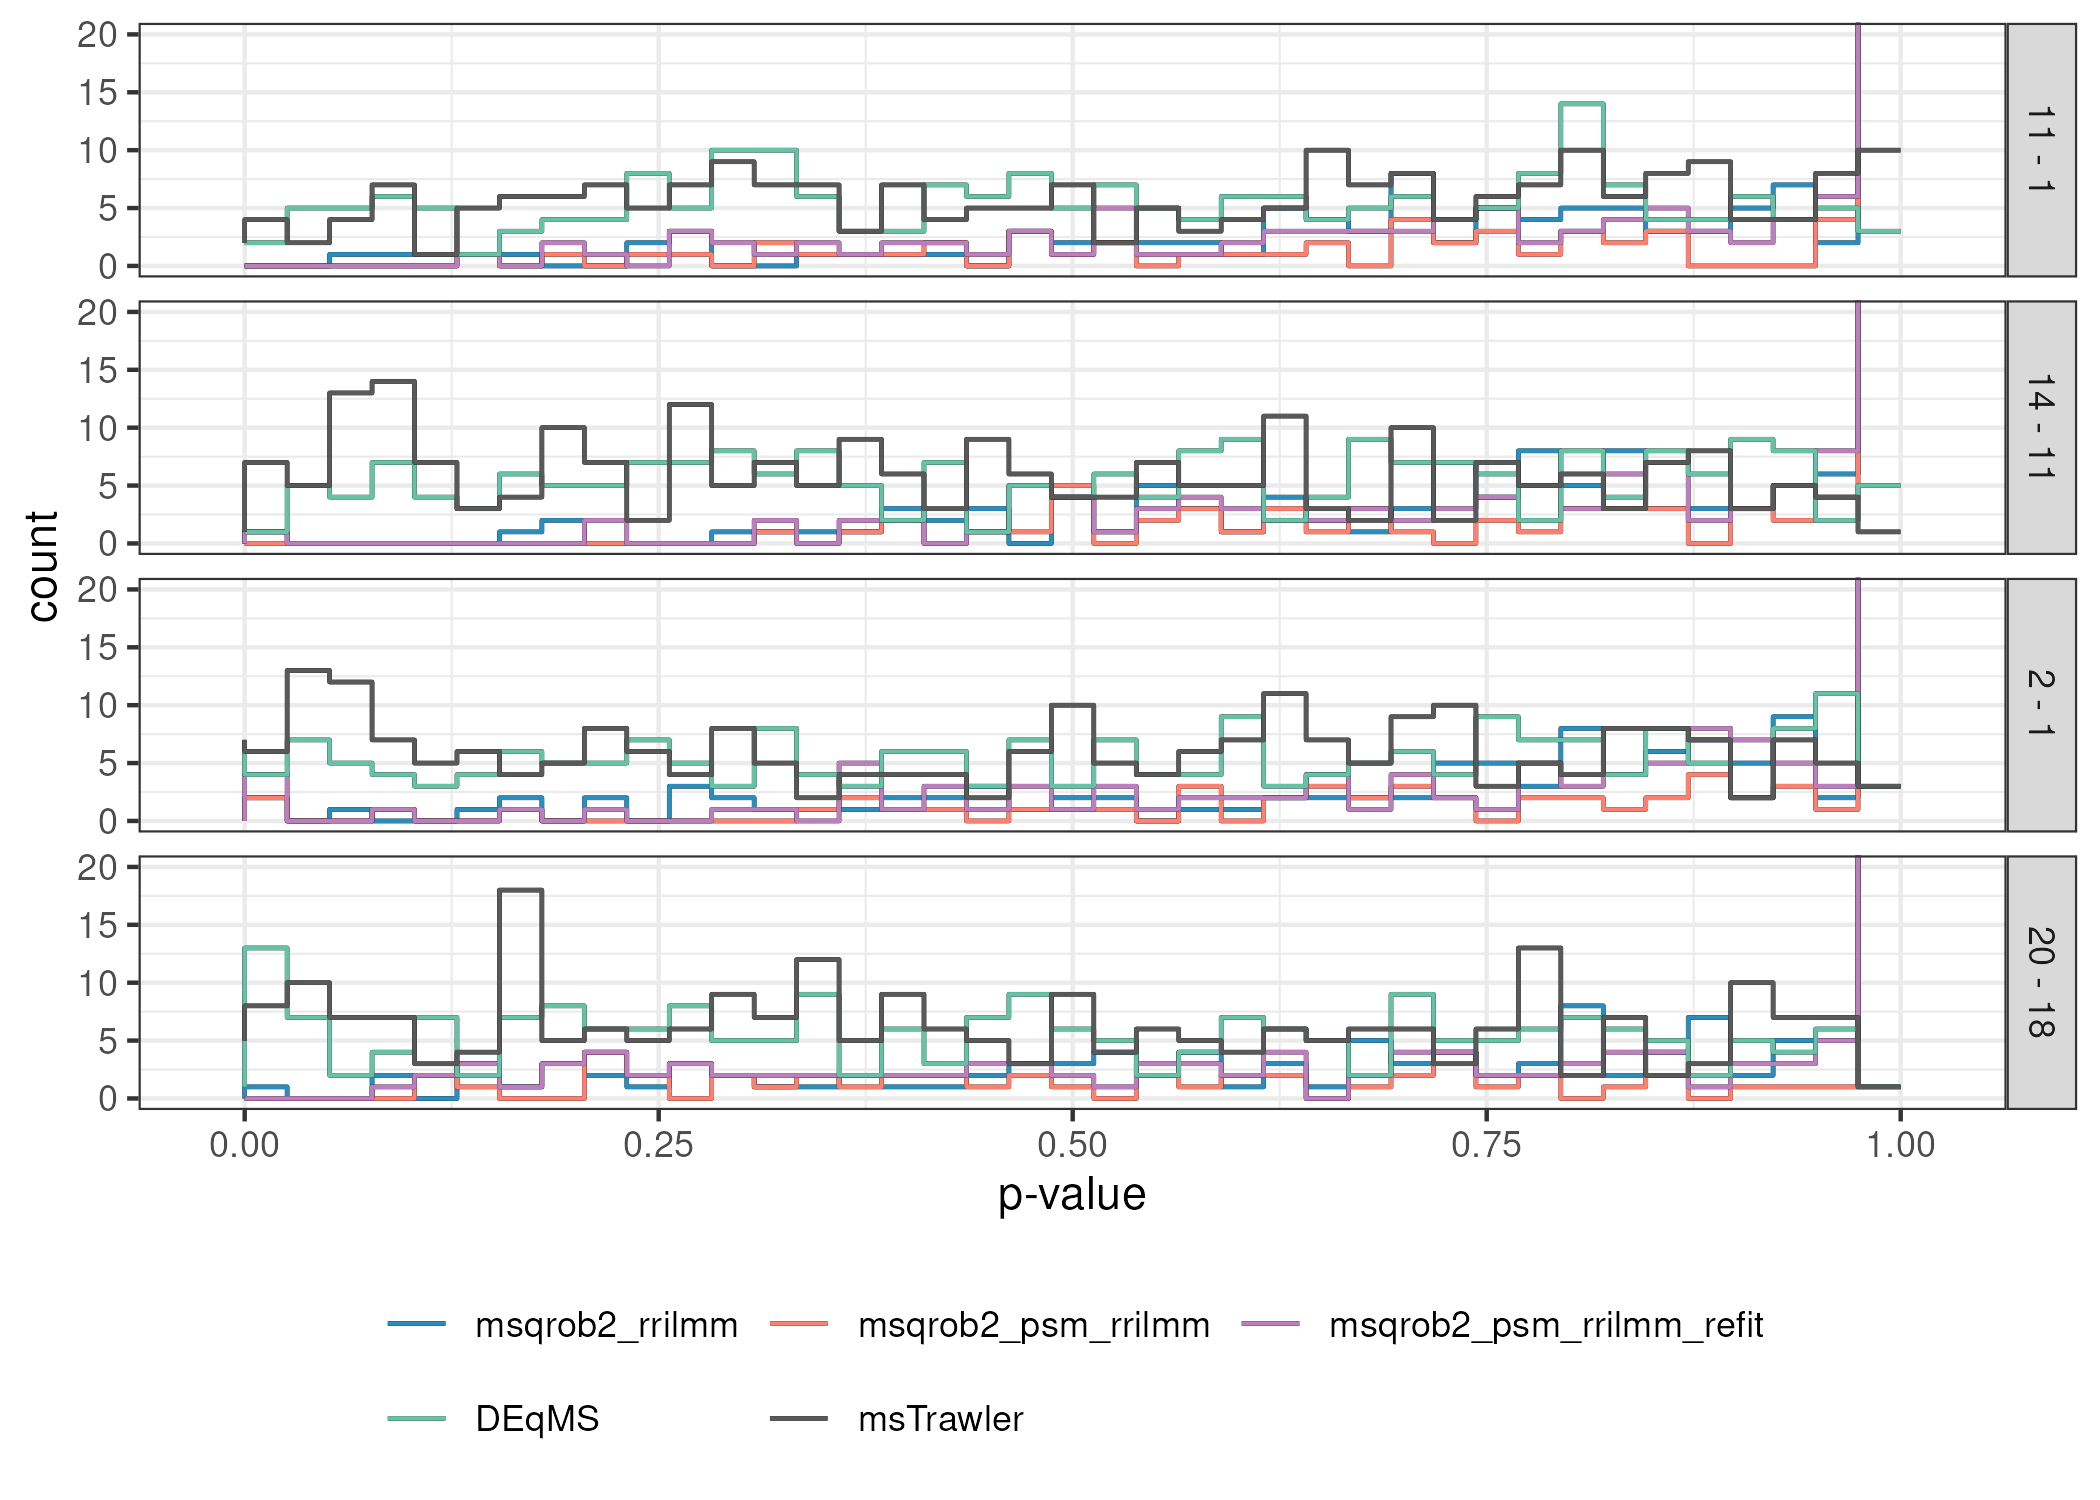
\includegraphics[width=1\textwidth,height=\textheight]{../figs/figureS10.png}

}

\caption{\label{fig-spikein2_pvalue_dist_nondiff}Histograms of the
p-values from non-spike-in proteins for the DEqMS, msqrob2TMT, and
msTrawler workflows for four distinct pairwise comparisons between
spike-in dilutions.}

\end{figure}%

\section*{Mouse Study}

\begin{figure}[H]

\centering{

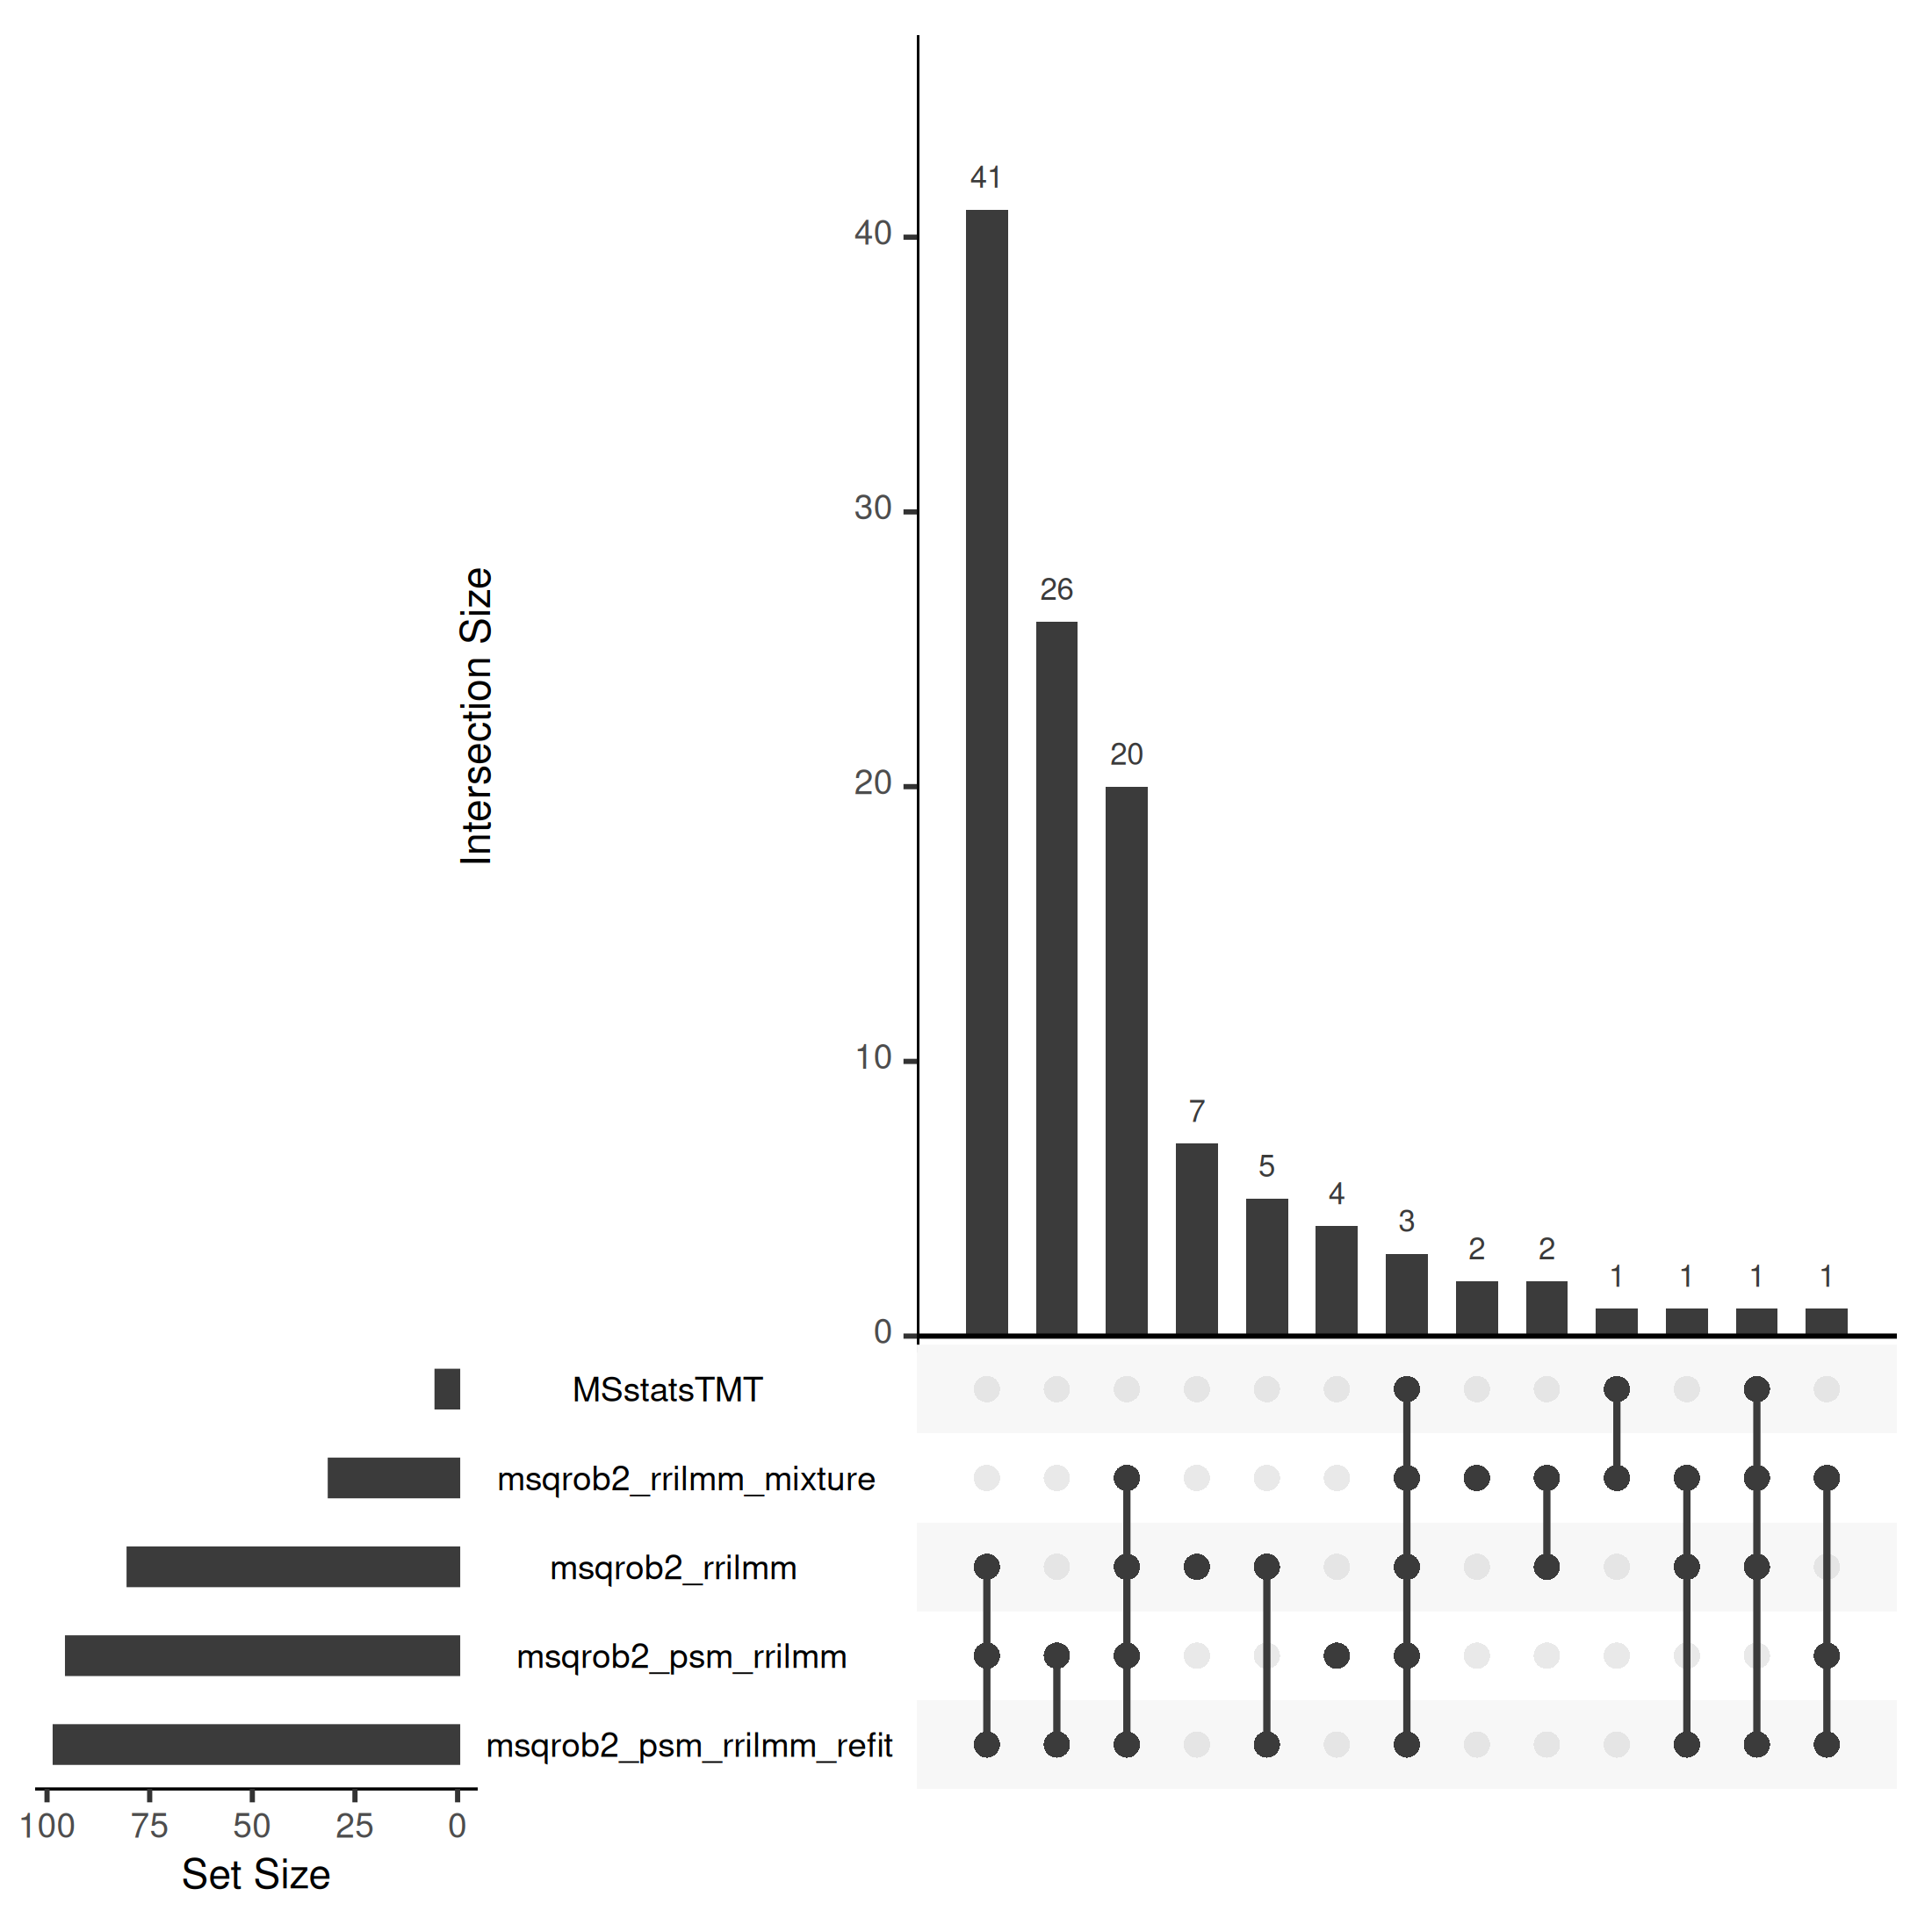
\includegraphics[width=1\textwidth,height=\textheight]{../figs/figureS11.png}

}

\caption{\label{fig-Upset-early}Upset plot showing the overlap in
significant proteins between the MSstatsTMT and the msqrob2TMT workflows
for the early diet effect.}

\end{figure}%

\begin{figure}[H]

\centering{

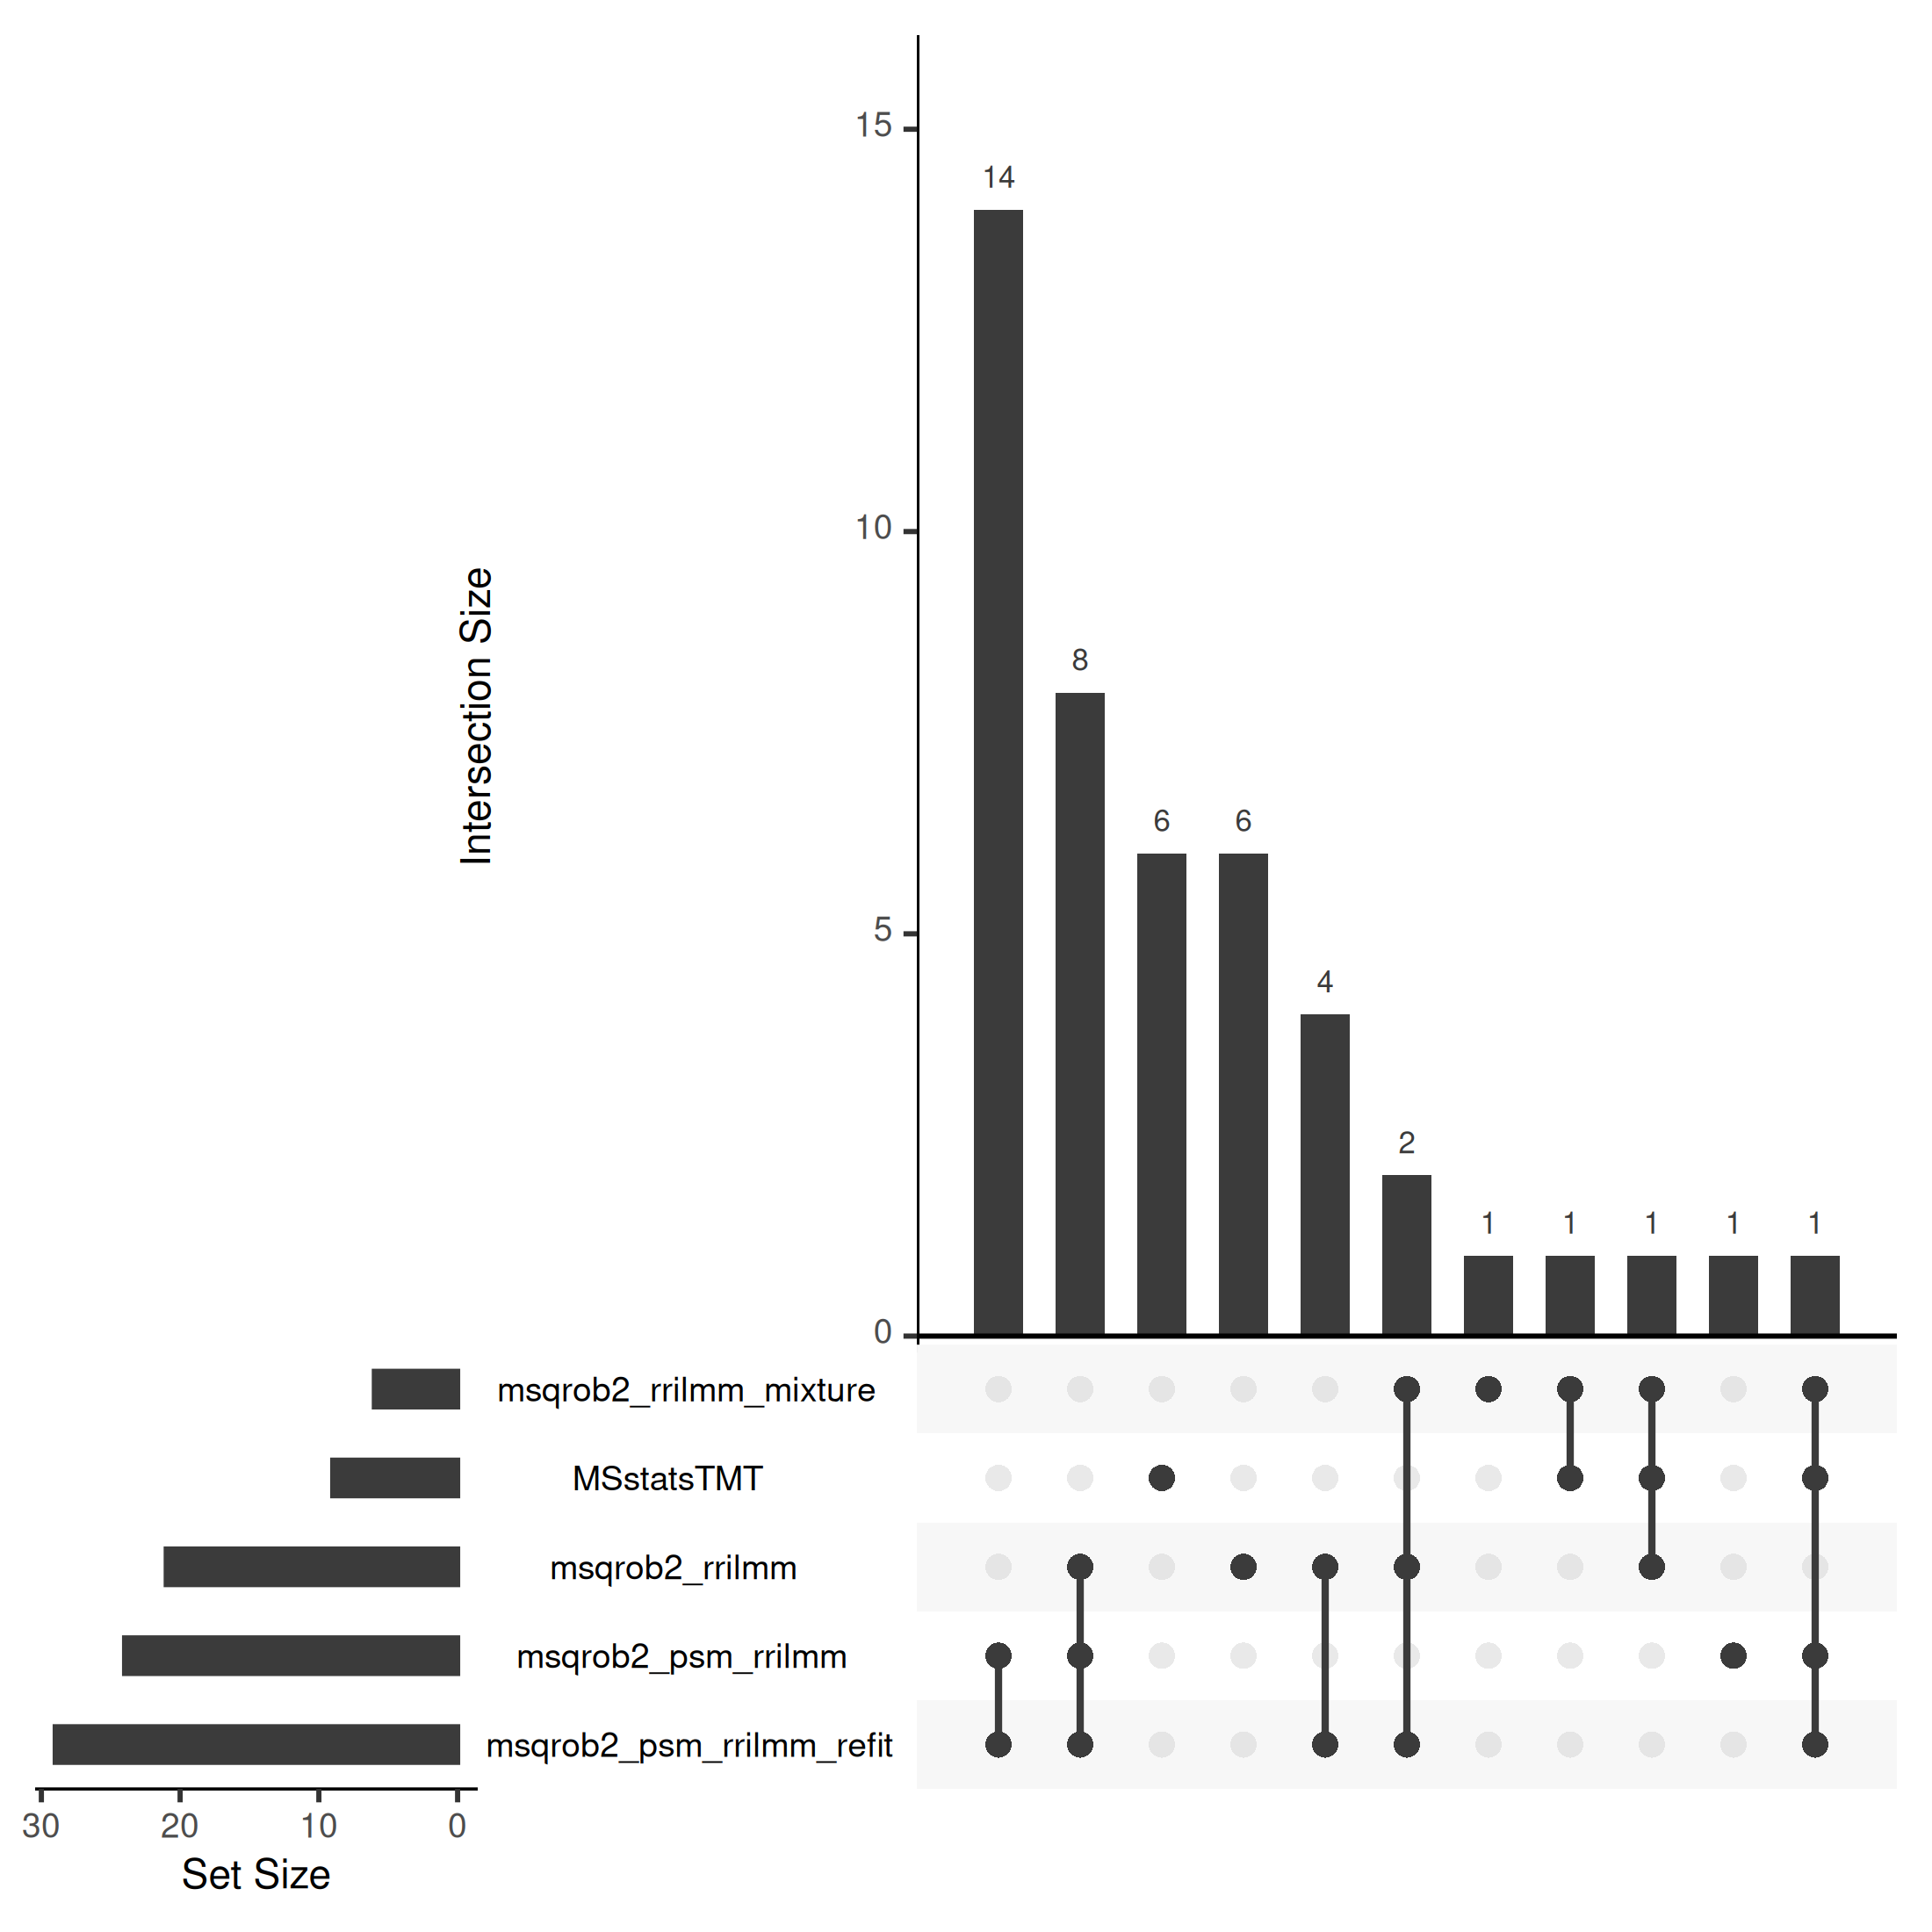
\includegraphics[width=1\textwidth,height=\textheight]{../figs/figureS12.png}

}

\caption{\label{fig-Upset-late}Upset plot showing the overlap in
significant proteins between the MSstatsTMT and the msqrob2TMT workflows
for the late diet effect.}

\end{figure}%

\begin{figure}[H]

\centering{

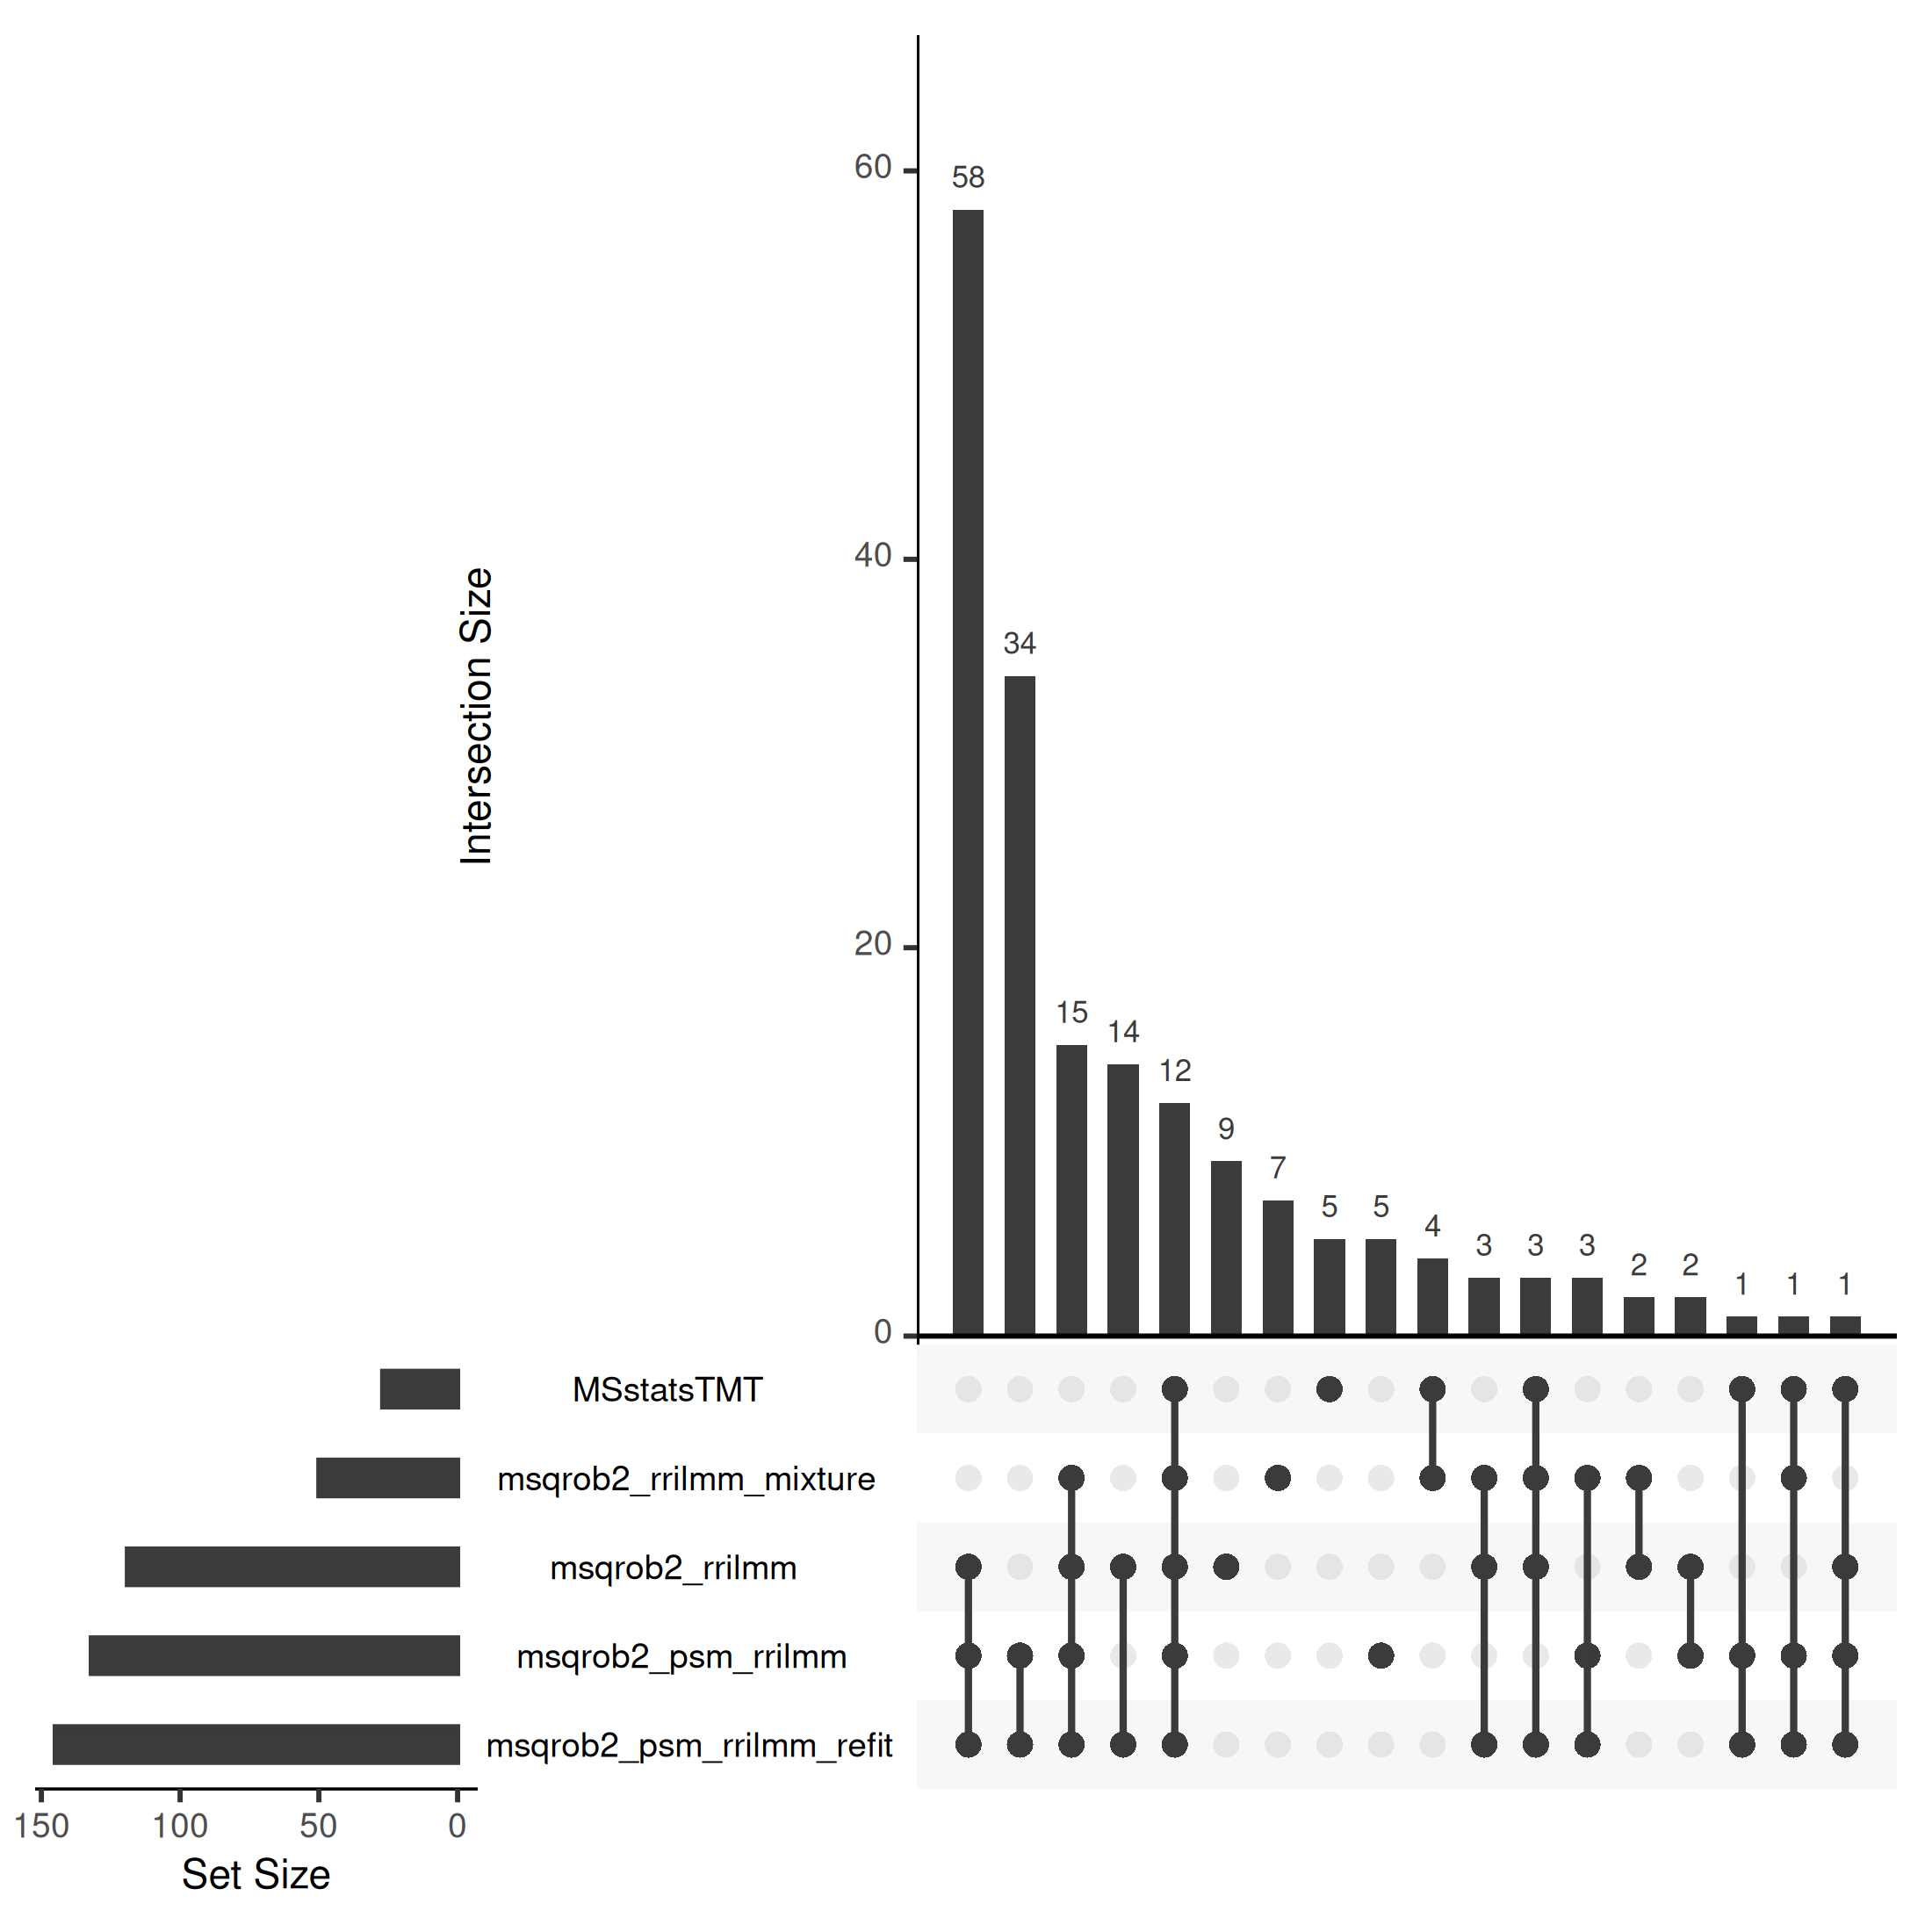
\includegraphics[width=1\textwidth,height=\textheight]{../figs/figureS13.png}

}

\caption{\label{fig-Upset-avg}Upset plot showing the overlap in
significant proteins between the MSstatsTMT and the msqrob2TMT workflows
for the average diet effect.}

\end{figure}%

\begin{figure}[H]

\centering{

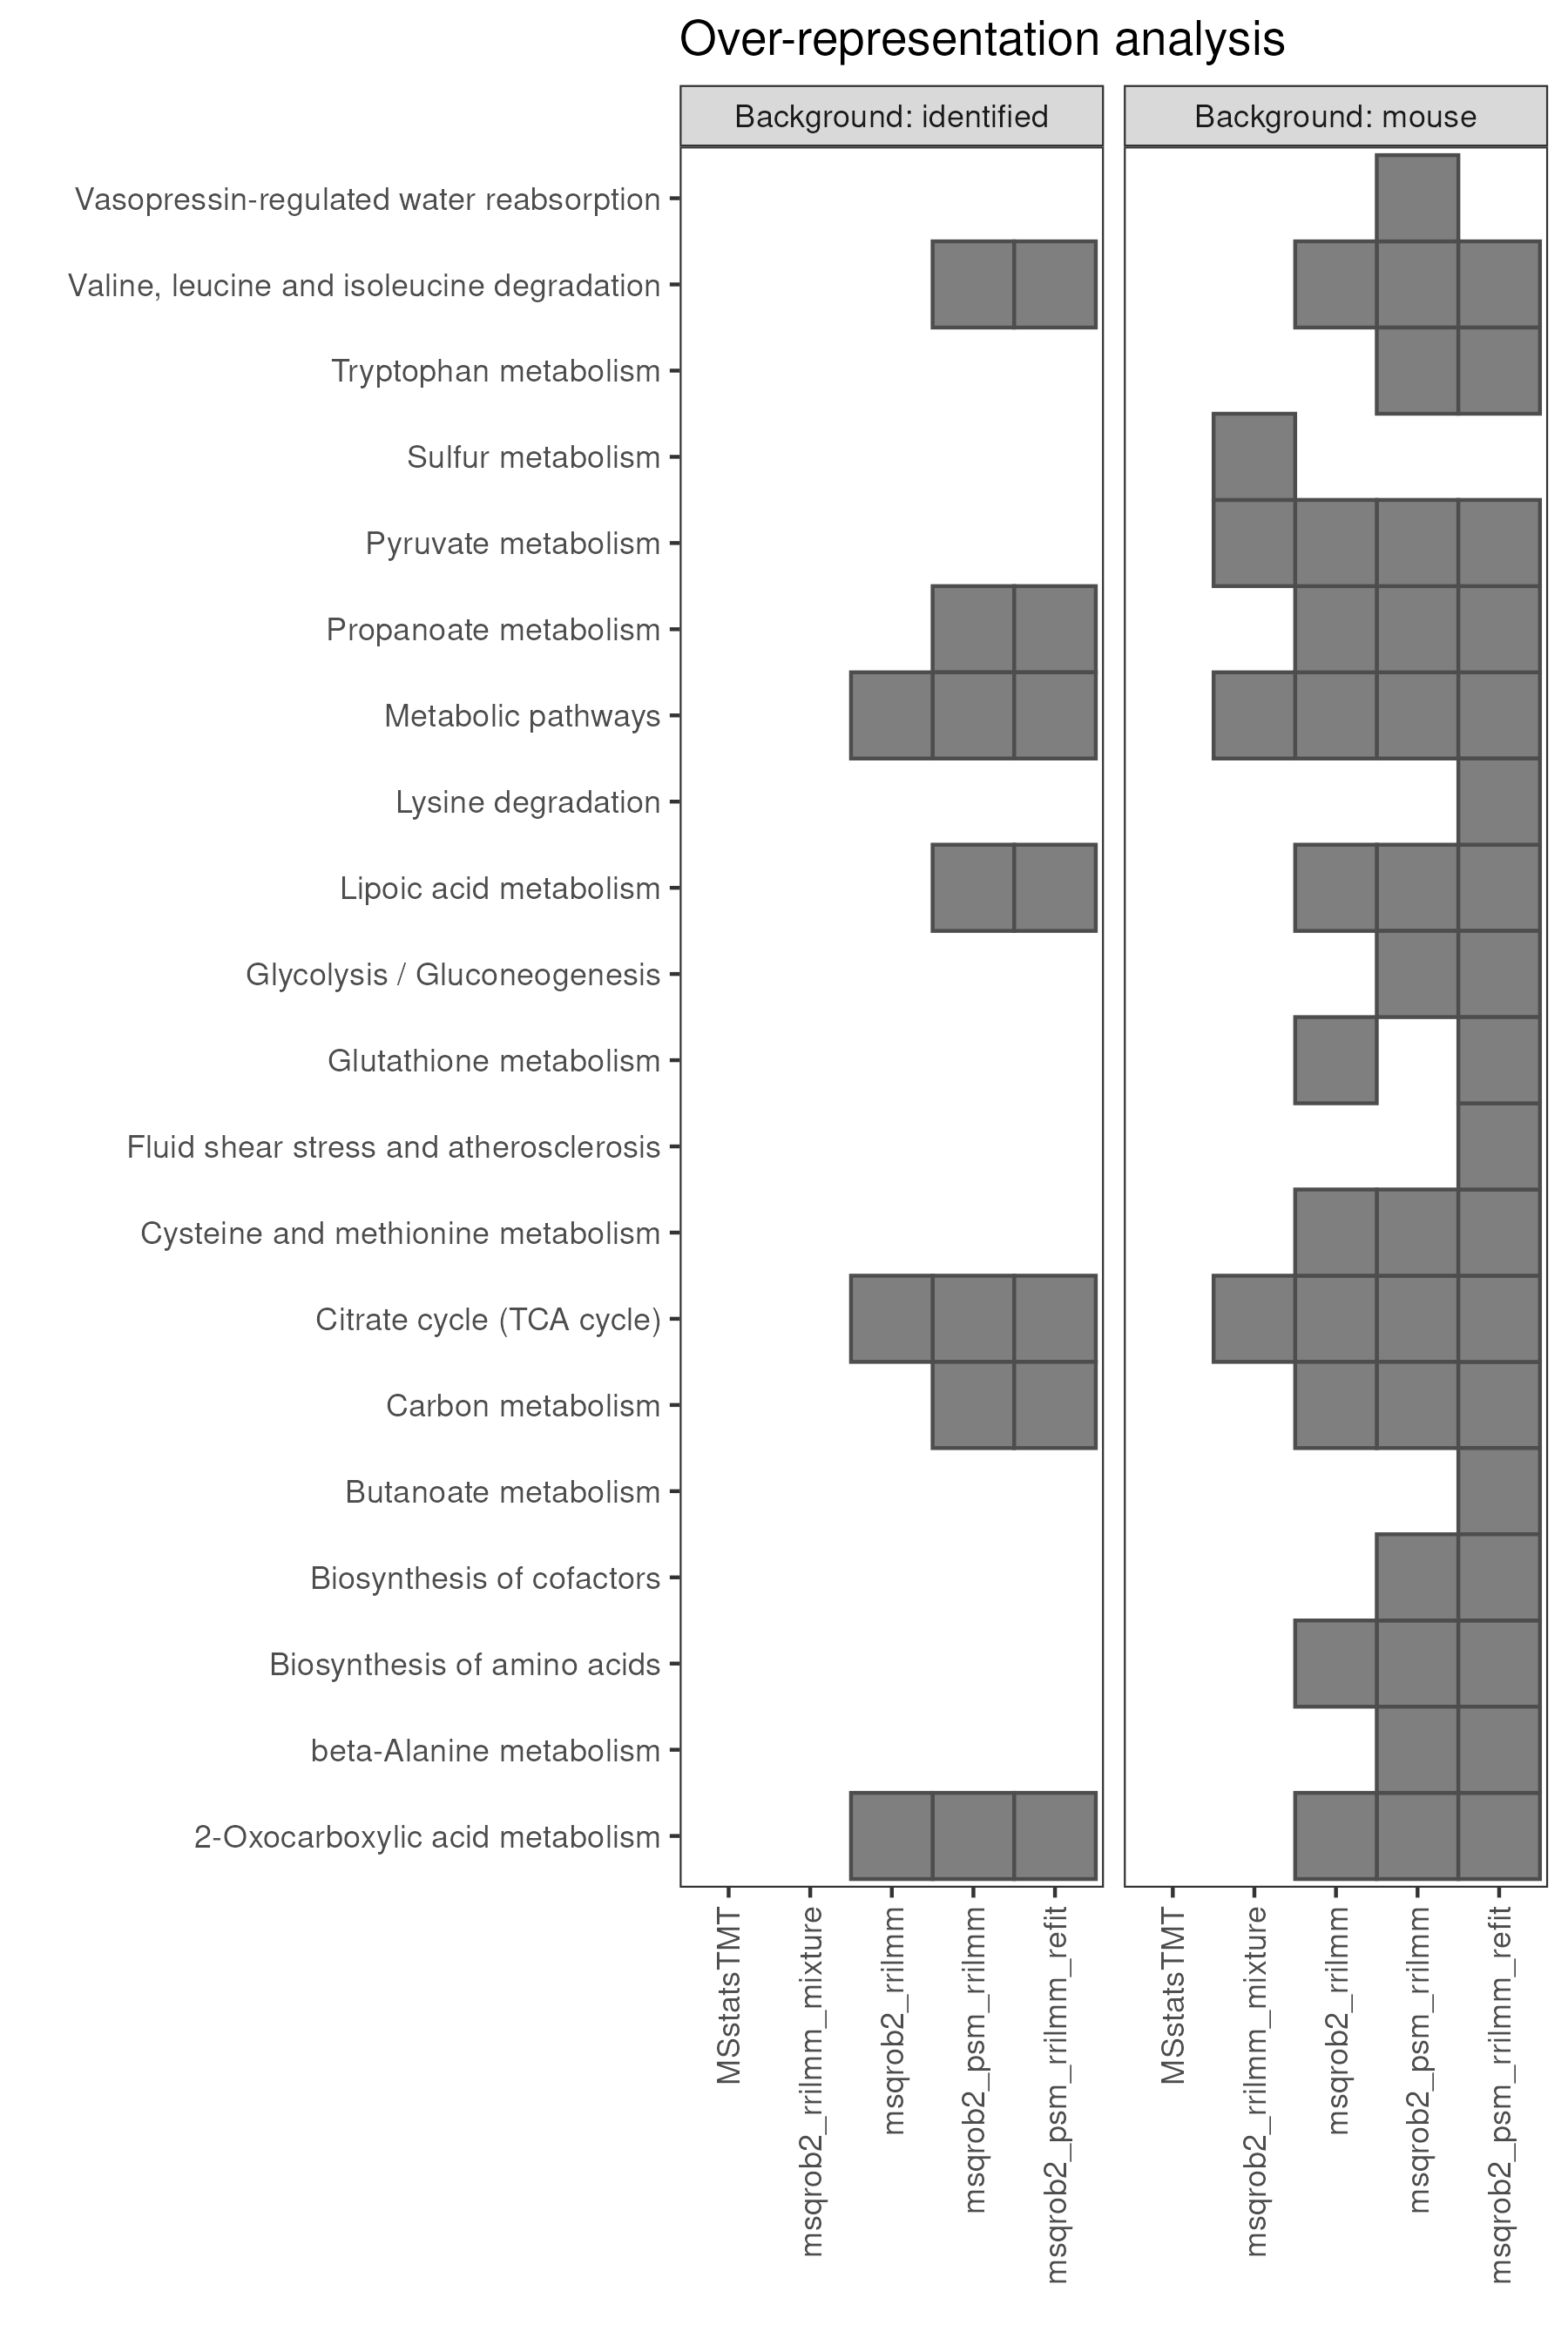
\includegraphics[width=0.7\textwidth,height=\textheight]{../figs/figureS14.png}

}

\caption{\label{fig-ora}Over-representation analysis on the set of
proteins identified as significant at a 5\% FDR threshold by each
method. Annotated protein sets were retrieved from KEGG. The significant
proteins were tested for over-representation against either the set of
identified proteins in the data set (left) or against the complete mouse
proteome. Grey boxes indicate that a KEGG protein set (rows) were
identified as over-represented by significant proteins identified by a
method (column). The proteins identified by MSstatsTMT did not lead to
significant KEGG pathway enrichment, hence the corresponding empty
columns.}

\end{figure}%

\begin{figure}

\centering{

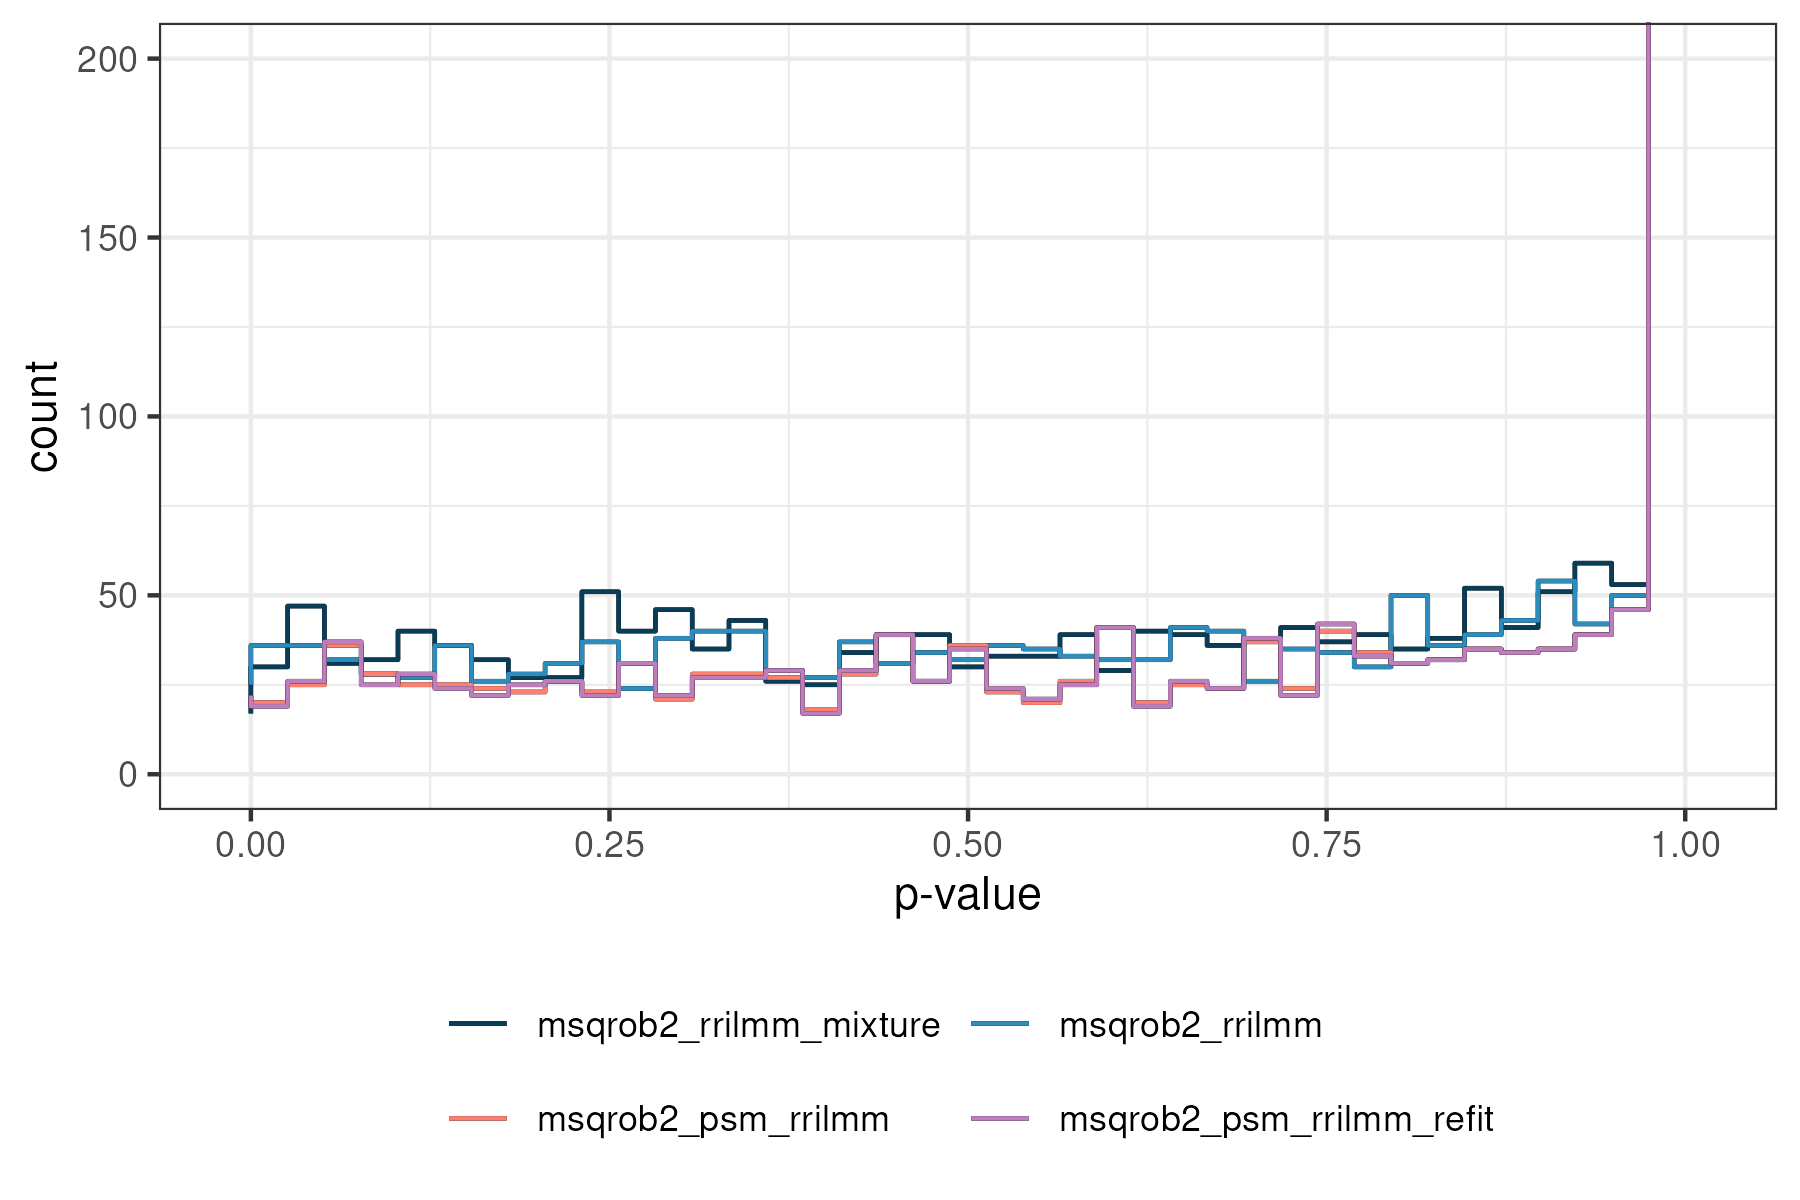
\includegraphics[width=1\textwidth,height=\textheight]{../figs/figureS15.png}

}

\caption{\label{fig-mouse-mock-pval}Histogram of the p-values from the
mock analysis on the mouse dataset. Only results for our PSM-level and
protein-level msqrob2TMT workflows are shown, as the state-of-the-art
tools could not fit the appropriate models to the data of the mouse
study after including an additional mock treatment.''}

\end{figure}%




\end{document}
